\documentclass[11pt]{article}

\usepackage[margin=2.5cm]{geometry}
\usepackage{amsmath,amssymb,amsthm}
\usepackage{booktabs}
\usepackage{graphicx}
\usepackage{mathtools}
\usepackage{longtable}
% \usepackage{xr-hyper}  % disabled for arXiv (cross-refs hardcoded)
\usepackage{hyperref}
\hypersetup{colorlinks=true,linkcolor=blue,citecolor=blue,urlcolor=blue}

% Cross-reference main paper
% (commented out for arXiv: absolute path; refs hardcoded below)
% \externaldocument{/home/isaia/Write/GKW/GKW1/Gauss}

\newtheorem{theorem}{Theorem}

% Supplementary material numbering: prefix all counters with S
\renewcommand{\thetable}{S\arabic{table}}
\renewcommand{\thefigure}{S\arabic{figure}}
\renewcommand{\theequation}{S\arabic{equation}}
\renewcommand{\thetheorem}{S\arabic{theorem}}

\title{Supplementary Material:\\Certified spectral enclosures for transfer operators and the Gauss map}
\author{Isaia Nisoli}
\date{}

\begin{document}
\maketitle

% Script 1: full_certification_50eigs.jl (resolvent certification, all 50 eigenvalues)
% Script 2: spectral_data_50eigs.jl (ell_j(1) at K=256, BigFloat Schur)
% Script 3: bigfloat_spectral_K1024.jl (ell_j(1) at K=1024, 2048-bit precision)
% Script 4: bigfloat_spectral_K1024.jl (ell_j(1) at K=1024, 2048-bit precision)

\subsection*{Notation}

Throughout this supplement we work exclusively on the Hardy space $H^2(D_1)$
and with the endomorphism $L := S\mathcal L : H^2(D_1) \to H^2(D_1)$
(see \S2 of the main paper).
All operator norms $\|\cdot\|$ are the $H^2(D_1)$ operator norm;
since the shifted monomials $\{(w-1)^n\}$ form an orthonormal basis in $H^2(D_1)$,
the matrix norm coincides with the Euclidean spectral norm $\|\cdot\|_2$.
We write $L_K := \Pi_K L$ for the Galerkin truncation of rank $K+1$,
and $\varepsilon_K := \|L - L_K\| \leq C_2 (2/3)^{K+1}$ for
the truncation error.

\subsection*{Computational environment}

All computations were performed on a single workstation with the following specifications:
\begin{itemize}
\item \textbf{Processor:} AMD Ryzen 9 5950X (16 cores, 32 threads via SMT, base 3.4\,GHz / boost 4.9\,GHz)
\item \textbf{Memory:} 128\,GB DDR4
\item \textbf{OS:} Ubuntu 22.04.5 LTS (kernel 6.8.0-79)
\item \textbf{Software:} Julia 1.12.4 with 32 threads; packages: GKWExperiments.jl, BallArithmetic.jl, GenericSchur.jl, ArbNumerics.jl
\end{itemize}

\begin{table}[ht]
\centering
\caption{Computational timings for each stage of the certification pipeline.
Timings with ``(cached)'' indicate that the BallMatrix or Schur decomposition was loaded from a previous run.}
\label{S-tab:timings}
\begin{tabular}{lp{7.5cm}r}
\toprule
Phase & Description & Wall time \\
\midrule
\multicolumn{3}{l}{\emph{Script 1: Resolvent certification (\texttt{full\_certification\_50eigs.jl})}} \\
\quad 1a & CertifScripts on full $L_{48}$ ($j = 1$--$15$) & $<\!1$\,min \\
\quad 1b & Block Schur + CertifScripts on $T_{22}$, $K\!=\!256$ ($j = 21$--$50$) & $<\!1$\,min \\
\quad 1c & Fallback: block Schur + CertifScripts, $K\!=\!256$ ($j = 16$--$20$) & ${\sim}\,2$\,min \\
\quad 2 & Transfer bridge + projector errors & $<\!1$\,min \\
\quad 3 & Tail resolvent on separating circle & ${\sim}\,32$\,s \\
\quad Total & & ${\sim}\,2.5$\,min \\
\midrule
\multicolumn{3}{l}{\emph{Script 2: Spectral coefficients (\texttt{spectral\_data\_50eigs.jl})}} \\
\quad Schur & BigFloat Schur, $K\!=\!256$, 512-bit (GenericSchur) & ${\sim}\,20$\,min \\
\quad ordschur & $\ell_j(\mathbf{1})$ via ordschur + triangular Sylvester ($50$ eigs) & ${\sim}\,2$\,min \\
\midrule
\multicolumn{3}{l}{\emph{Script 3: $K\!=\!1024$ spectral (\texttt{bigfloat\_spectral\_K1024.jl})}} \\
\quad Build & ArbNumerics matrix, $K\!=\!1024$, 2048-bit & ${\sim}\,25$\,min \\
\quad Schur & $1025 \times 1025$ GenericSchur at 2048-bit & ${\sim}\,18$\,hr \\
\quad Quality & Residual + orthogonality norms & ${\sim}\,2$\,hr \\
\quad ordschur & $50 \times$ ordschur + Sylvester + perturbation & ${\sim}\,1$\,hr \\
\quad Total & & ${\sim}\,21$\,hr \\
\bottomrule
\end{tabular}
\end{table}

\subsection*{Data availability}

All certified spectral data (eigenvalue enclosures, eigenvector coefficients,
Riesz projector norms, and spectral expansion coefficients) are available in
machine-readable form at the Harvard Dataverse:
\url{https://doi.org/10.7910/DVN/HKM3Y2}.

\subsection*{Computational methodology}

The certification pipeline is implemented in two Julia packages:
\texttt{GKWExperiments.jl} (operator-specific discretization and lift)
and \texttt{BallArithmetic.jl} (validated linear algebra: Schur certification,
resolvent bounds, spectral norm enclosures).
Below we describe the role of each script and the main functions it calls.

\paragraph{Script~1: Resolvent certification (\texttt{full\_certification\_50eigs.jl}).}
This script certifies the resolvent of the infinite-dimensional operator
on $50$ excluding circles $\Gamma_j$ via the two-stage strategy
of \S3.3 of the main paper, and computes the Riesz projector errors.

\begin{description}
\item[Phase~0: Matrix construction.]
  \texttt{gkw\_matrix\_direct(s; K=K)} builds the $(K{+}1)\times(K{+}1)$
  Galerkin matrix in Arb arithmetic (ArbNumerics.jl).
  The truncation error $\varepsilon_K = C_2\,(2/3)^{K+1}$ is computed by
  \texttt{compute\_C2} and \texttt{compute\_\(\Delta\)}.
  The Arb matrix is converted to \texttt{BallMatrix(BigFloat, M\_arb)}
  for validated linear algebra.

\item[Phase~1a: Circle sampling at $K = 48$.]
  For $j = 1, \ldots, 15$, the resolvent $\|(zI - L_{48})^{-1}\|$
  is sampled at $256$ equally-spaced points on $\Gamma_j$ using
  \texttt{CertifScripts.run\_certification}.
  This function computes a certified Schur decomposition $L_K = QTQ^*$
  (\texttt{compute\_schur\_and\_error}),
  bounds the resolvent via
  Theorem~3.4 of the main paper
  (\texttt{schur\_to\_original\_resolvent}),
  and returns the supremum $\sup_{z\in\Gamma_j}\|R_{L_K}(z)\|$.
  The small-gain factor $\alpha_j = \varepsilon_{48}\cdot\sup\|R_{L_{48}}\|$
  is computed with directed rounding (\texttt{setrounding(Float64, RoundUp)}).

\item[Phase~1b: Block Schur at $K = 256$.]
  For $j = 16, \ldots, 50$, the resolvent of $L_{48}$ is too large.
  Instead, \texttt{certify\_eigenvalue\_schur\_direct}
  computes a BigFloat Schur form $L_{256} = QTQ^*$ (GenericSchur.jl),
  partitions $T$ around $\lambda_j$ (Lemma~3.5),
  and certifies the resolvent supremum on $\Gamma_j$
  via Proposition~3.7.
  The Schur similarity defect is bounded by
  Lemma~3.1.

\item[Phase~2: Infinite-dimensional lift.]
  For each eigenvalue, the certified finite-dimensional resolvent
  is lifted to $L$ via the Neumann perturbation bound
  $M_{\infty,j} = \|R_{L_K}\|/(1 - \alpha_j)$.
  The Riesz projector error $\vartheta_j$ is computed by
  \texttt{projector\_approximation\_error\_rigorous},
  and the eigenvalue enclosure follows from
  Lemma~2.12:
  $|\lambda_j - \hat\lambda_j| \leq
   (\varepsilon_K(1{+}\vartheta_j) + 2C\vartheta_j)/(1{-}\vartheta_j)$.

\item[Phase~3: Tail resolvent.]
  A separating circle $|z| = \rho$ in the eigenvalue gap
  $|\lambda_{51}| < \rho < |\lambda_{50}|$ is chosen, and the resolvent
  $\|R_L\|$ on this circle is certified by the same block Schur
  method, giving the tail bound constant $M_\infty$.
\end{description}

\paragraph{Script~3: Spectral coefficients (\texttt{bigfloat\_spectral\_K1024.jl}).}
This script computes the spectral coefficients $\ell_j(\mathbf{1})$
at $K = 1024$ with $2048$-bit precision, following the certified Schur
pipeline of \S3.4 of the main paper.

\begin{description}
\item[Step~1: BallMatrix construction.]
  \texttt{gkw\_matrix\_direct\_fast(s; K=1024, threaded=true)} builds
  the Arb matrix in $O(K^3)$ operations.
  Conversion via \texttt{BallMatrix(BigFloat, M\_arb)}
  preserves all $2048$ bits of center precision
  (no Float64 truncation).

\item[Step~2: BigFloat Schur decomposition.]
  \texttt{GenericSchur.schur} computes $L_K = QTQ^*$ at $2048$-bit precision.
  The Schur residual $\|L_K - QTQ^*\|$ and orthogonality defect
  $\|Q^*Q - I\|$ are certified via
  \texttt{upper\_bound\_L2\_opnorm(BallMatrix(\ldots))},
  giving the total enclosure error $\|E\|$
  (Lemma~3.1).

\item[Step~3: Ordered Schur and triangular solve.]
  For each $j = 1, \ldots, 50$, \texttt{bigfloat\_ordschur}
  reorders the Schur form to place $\lambda_j$ in position $(1,1)$
  via Givens rotations.
  The spectral coefficient is extracted by the direct triangular solve:
  $q = \overline{Q_{\mathrm{ord},1,:}}$,\;
  $z = (T_{22} - \lambda_j I)^{-1} q_{\mathrm{rest}}$,\;
  $\ell_j(\mathbf{1}) = \mathrm{Re}(q_1 - \sum_i T_{12,i}\,z_i)$.
  The ordschur quality (reordering residual and orthogonality)
  is tracked via \texttt{upper\_bound\_L2\_opnorm}.

\item[Step~4: Perturbation bound.]
  The total certified error $\delta$ on $\ell_j(\mathbf{1})$
  is dominated by the Schur similarity defect $\|E\|$;
  the triangular solve residual is negligible
  ($\sim 10^{-309}$ at $1024$-bit).
  Sign certification holds when $|\ell_j(\mathbf{1})| > \delta$.
\end{description}

An analogous script \texttt{bigfloat\_spectral\_K1024.jl}
performs the same computation at $K = 1024$ with $2048$-bit precision
for cross-validation.

\paragraph{Tail bound (\texttt{compute\_tail\_bound\_N50.jl}).}
This script computes the rigorous tail bound for the spectral remainder
$R_{50}(n)$.
It loads the certified spectral data from Script~3 and the tail
resolvent from Script~1, constructs componentwise ball vectors for
each Riesz projector $P_j(\mathbf{1})$ ($j = 1, \ldots, 50$),
computes the tail projection $Q_{50}\mathbf{1} = \mathbf{1} - \sum_j P_j\mathbf{1}$
using interval arithmetic with directed rounding (triangle inequality),
and adds an infinite-dimensional correction
$\sum_j \varepsilon_K / \mathrm{sep}_j$ to lift from the Galerkin
approximation $L_K$ to the full operator $L$.
The final output is
$\|R_{50}(n)\| \leq \rho^{n+1} \cdot M_\infty \cdot \|Q_{50}\mathbf{1}\|$.

\begin{table}[ht]
\centering
\caption{Two-stage certification parameters}
\label{S-tab:two-stage-params}
\begin{tabular}{ll}
\toprule
Parameter & Value \\
\midrule
$K_{\mathrm{low}}$ & $48$ (eigenvalues $1$--$15$), $256$ (eigenvalues $16$--$50$) \\
$K_{\mathrm{high}}$ & $256$ \\
$C_2$ & $1.005810 \times 10^{1}$ \\
$\varepsilon_{48}$ & $2.366161 \times 10^{-8}$ \\
$\varepsilon_{256}$ & $5.585504 \times 10^{-45}$ \\
Circle samples & $256$ \\
Method ($j = 1$--$15$) & CertifScripts circle certification on full $L_{48}$ \\
Method ($j = 16$--$50$) & Block Schur at $K = 256$ + CertifScripts on $T_{22}$ \\
\bottomrule
\end{tabular}
\end{table}

\begin{longtable}{rlcccccc}
\caption{Two-stage certification results for the first $50$ eigenvalues of the GKW operator ($s=1$).
The column $\alpha_1 = \varepsilon_{K_{\mathrm{low}}} \cdot \|R_{L_{K_{\mathrm{low}}}}(z)\|$ is the
small-gain factor on the excluding circle $\Gamma_j$.  All $50$ eigenvalues satisfy $\alpha_1 < 1$,
proving simplicity and giving certified resolvent bounds.
The ``Eval.~encl.'' column gives the eigenvalue error radius from
projector control (Lemma~2.12).
For $j = 1$--$15$, resolvent sampling on the full $L_{48}$;
for $j = 16$--$50$, block Schur at $K = 256$ with certified resolvent on $T_{22}$.}
\label{S-tab:two-stage-results}\\
\toprule
$j$ & $\hat\lambda_j$ & $K_{\mathrm{low}}$ & $\alpha_1$ & Circle $r$ & Eval.~encl. & Riesz proj.~err \\
\midrule
\endfirsthead
\multicolumn{7}{c}{\textit{continued}} \\
\toprule
$j$ & $\hat\lambda_j$ & $K_{\mathrm{low}}$ & $\alpha_1$ & Circle $r$ & Eval.~encl. & Riesz proj.~err \\
\midrule
\endhead
1 & $+1.0000000000$ & 48 & $1.01 \times 10^{-5}$ & $1.00 \times 10^{-2}$ & $7.40 \times 10^{-45}$ & $1.01 \times 10^{-41}$ \\
2 & $-0.3036630029$ & 48 & $3.53 \times 10^{-5}$ & $3.04 \times 10^{-3}$ & $2.33 \times 10^{-44}$ & $3.77 \times 10^{-41}$ \\
3 & $+0.1008845093$ & 48 & $1.11 \times 10^{-4}$ & $1.01 \times 10^{-3}$ & $7.32 \times 10^{-44}$ & $1.23 \times 10^{-40}$ \\
4 & $-0.0354961590$ & 48 & $3.24 \times 10^{-4}$ & $3.55 \times 10^{-4}$ & $2.17 \times 10^{-43}$ & $3.73 \times 10^{-40}$ \\
5 & $+0.0128437904$ & 48 & $9.15 \times 10^{-4}$ & $1.28 \times 10^{-4}$ & $6.22 \times 10^{-43}$ & $1.08 \times 10^{-39}$ \\
6 & $-4.7177775e-03$ & 48 & $2.52 \times 10^{-3}$ & $4.72 \times 10^{-5}$ & $1.75 \times 10^{-42}$ & $3.01 \times 10^{-39}$ \\
7 & $+1.7486751e-03$ & 48 & $6.85 \times 10^{-3}$ & $1.75 \times 10^{-5}$ & $4.85 \times 10^{-42}$ & $8.29 \times 10^{-39}$ \\
8 & $-6.5202086e-04$ & 48 & $1.84 \times 10^{-2}$ & $6.52 \times 10^{-6}$ & $1.33 \times 10^{-41}$ & $2.29 \times 10^{-38}$ \\
9 & $+2.4413147e-04$ & 48 & $4.91 \times 10^{-2}$ & $2.44 \times 10^{-6}$ & $3.63 \times 10^{-41}$ & $6.49 \times 10^{-38}$ \\
10 & $-9.1689084e-05$ & 48 & $1.30 \times 10^{-1}$ & $9.17 \times 10^{-7}$ & $9.85 \times 10^{-41}$ & $2.05 \times 10^{-37}$ \\
11 & $+3.4516546e-05$ & 48 & $3.44 \times 10^{-1}$ & $3.45 \times 10^{-7}$ & $2.66 \times 10^{-40}$ & $9.48 \times 10^{-37}$ \\
12 & $-1.3017698e-05$ & 48 & $4.99 \times 10^{-1}$ & $2.37 \times 10^{-7}$ & $7.16 \times 10^{-40}$ & $2.34 \times 10^{-36}$ \\
13 & $+4.9167823e-06$ & 48 & $4.97 \times 10^{-1}$ & $2.37 \times 10^{-7}$ & $1.92 \times 10^{-39}$ & $2.31 \times 10^{-36}$ \\
14 & $-1.8593074e-06$ & 48 & $5.01 \times 10^{-1}$ & $2.37 \times 10^{-7}$ & $5.15 \times 10^{-39}$ & $2.38 \times 10^{-36}$ \\
15 & $+7.0381134e-07$ & 48 & $6.21 \times 10^{-1}$ & $2.01 \times 10^{-7}$ & $1.38 \times 10^{-38}$ & $5.36 \times 10^{-36}$ \\
\midrule
16 & $-2.6664134e-07$ & 256 & $8.11 \times 10^{-32}$ & $1.14 \times 10^{-7}$ & $3.67 \times 10^{-38}$ & $1.34 \times 10^{-25}$ \\
17 & $+1.0109055e-07$ & 256 & $5.48 \times 10^{-31}$ & $4.33 \times 10^{-8}$ & $9.78 \times 10^{-38}$ & $2.33 \times 10^{-24}$ \\
18 & $-3.8349698e-08$ & 256 & $3.70 \times 10^{-30}$ & $1.64 \times 10^{-8}$ & $2.60 \times 10^{-37}$ & $4.02 \times 10^{-23}$ \\
19 & $+1.4556138e-08$ & 256 & $2.50 \times 10^{-29}$ & $6.23 \times 10^{-9}$ & $6.91 \times 10^{-37}$ & $6.96 \times 10^{-22}$ \\
20 & $-5.5275679e-09$ & 256 & $1.69 \times 10^{-28}$ & $2.36 \times 10^{-9}$ & $1.84 \times 10^{-36}$ & $1.20 \times 10^{-20}$ \\
21 & $+2.0999136e-09$ & 256 & $1.14 \times 10^{-27}$ & $8.98 \times 10^{-10}$ & $4.87 \times 10^{-36}$ & $2.08 \times 10^{-19}$ \\
22 & $-7.9804577e-10$ & 256 & $7.68 \times 10^{-27}$ & $3.41 \times 10^{-10}$ & $1.29 \times 10^{-35}$ & $3.60 \times 10^{-18}$ \\
23 & $+3.0338629e-10$ & 256 & $5.18 \times 10^{-26}$ & $1.30 \times 10^{-10}$ & $3.41 \times 10^{-35}$ & $6.23 \times 10^{-17}$ \\
24 & $-1.1536954e-10$ & 256 & $3.49 \times 10^{-25}$ & $4.93 \times 10^{-11}$ & $9.02 \times 10^{-35}$ & $1.08 \times 10^{-15}$ \\
25 & $+4.3883450e-11$ & 256 & $2.36 \times 10^{-24}$ & $1.88 \times 10^{-11}$ & $2.38 \times 10^{-34}$ & $1.87 \times 10^{-14}$ \\
26 & $-1.6696052e-11$ & 256 & $1.59 \times 10^{-23}$ & $7.14 \times 10^{-12}$ & $6.29 \times 10^{-34}$ & $3.25 \times 10^{-13}$ \\
27 & $+6.3536124e-12$ & 256 & $1.08 \times 10^{-22}$ & $2.72 \times 10^{-12}$ & $1.66 \times 10^{-33}$ & $5.67 \times 10^{-12}$ \\
28 & $-2.4183168e-12$ & 256 & $7.38 \times 10^{-22}$ & $1.03 \times 10^{-12}$ & $4.38 \times 10^{-33}$ & $1.01 \times 10^{-10}$ \\
29 & $+9.2062742e-13$ & 256 & $5.15 \times 10^{-21}$ & $3.94 \times 10^{-13}$ & $1.16 \times 10^{-32}$ & $1.87 \times 10^{-9}$ \\
30 & $-3.5053094e-13$ & 256 & $3.83 \times 10^{-20}$ & $1.50 \times 10^{-13}$ & $3.06 \times 10^{-32}$ & $3.93 \times 10^{-8}$ \\
31 & $+1.3348571e-13$ & 256 & $3.52 \times 10^{-19}$ & $5.71 \times 10^{-14}$ & $8.08 \times 10^{-32}$ & $1.26 \times 10^{-6}$ \\
32 & $-5.0839831e-14$ & 256 & $5.08 \times 10^{-17}$ & $2.17 \times 10^{-14}$ & $2.14 \times 10^{-31}$ & $1.00 \times 10^{-2}$ \\
33 & $+1.9365544e-14$ & 256 & $2.58 \times 10^{-18}$ & $8.28 \times 10^{-15}$ & $5.63 \times 10^{-31}$ & $9.86 \times 10^{-6}$ \\
34 & $-7.3774705e-15$ & 256 & $1.74 \times 10^{-17}$ & $3.15 \times 10^{-15}$ & $1.52 \times 10^{-30}$ & $1.71 \times 10^{-4}$ \\
35 & $+2.8108246e-15$ & 256 & $1.17 \times 10^{-16}$ & $1.20 \times 10^{-15}$ & $5.55 \times 10^{-30}$ & $2.96 \times 10^{-3}$ \\
\midrule
36 & $-1.0710387e-15$ & 256 & $7.90 \times 10^{-16}$ & $4.58 \times 10^{-16}$ & $\infty$ & $5.12 \times 10^{-2}$ \\
37 & $+4.0814893e-16$ & 256 & $5.33 \times 10^{-15}$ & $1.74 \times 10^{-16}$ & $\infty$ & $8.86 \times 10^{-1}$ \\
38 & $-1.5555055e-16$ & 256 & $3.59 \times 10^{-14}$ & $6.65 \times 10^{-17}$ & $\infty$ & $> 1$ \\
39 & $+5.9287246e-17$ & 256 & $2.42 \times 10^{-13}$ & $2.53 \times 10^{-17}$ & $\infty$ & $> 1$ \\
40 & $-2.2598811e-17$ & 256 & $1.63 \times 10^{-12}$ & $9.66 \times 10^{-18}$ & $\infty$ & $> 1$ \\
41 & $+8.6147444e-18$ & 256 & $1.10 \times 10^{-11}$ & $3.68 \times 10^{-18}$ & $\infty$ & $> 1$ \\
42 & $-3.2842013e-18$ & 256 & $7.41 \times 10^{-11}$ & $1.40 \times 10^{-18}$ & $\infty$ & $> 1$ \\
43 & $+1.2521200e-18$ & 256 & $4.99 \times 10^{-10}$ & $5.35 \times 10^{-19}$ & $\infty$ & $> 1$ \\
44 & $-4.7740757e-19$ & 256 & $3.36 \times 10^{-9}$ & $2.04 \times 10^{-19}$ & $\infty$ & $> 1$ \\
45 & $+1.8203644e-19$ & 256 & $2.27 \times 10^{-8}$ & $7.78 \times 10^{-20}$ & $\infty$ & $> 1$ \\
46 & $-6.9414738e-20$ & 256 & $1.53 \times 10^{-7}$ & $2.97 \times 10^{-20}$ & $\infty$ & $> 1$ \\
47 & $+2.6470860e-20$ & 256 & $1.03 \times 10^{-6}$ & $1.13 \times 10^{-20}$ & $\infty$ & $> 1$ \\
48 & $-1.0094998e-20$ & 256 & $6.93 \times 10^{-6}$ & $4.31 \times 10^{-21}$ & $\infty$ & $> 1$ \\
49 & $+3.8500394e-21$ & 256 & $4.66 \times 10^{-5}$ & $1.64 \times 10^{-21}$ & $\infty$ & $> 1$ \\
50 & $-1.4683981e-21$ & 256 & $3.14 \times 10^{-4}$ & $6.27 \times 10^{-22}$ & $\infty$ & $> 1$ \\
\bottomrule
\end{longtable}

\begin{longtable}{rlrrrr}
\caption{Certified resolvent bounds.  $\|R_{L_{K_{\mathrm{low}}}}\|$ is the resolvent of the
finite-dimensional Galerkin matrix on the excluding circle $\Gamma_j$, certified via
resolvent sampling (Phase~1a) or Schur direct method (Phase~1b/c).
$M_\infty = \|R_L(z)\|$ is the certified resolvent bound
for the infinite-dimensional operator via Neumann perturbation:
$M_\infty \leq \|R_{L_{K_{\mathrm{low}}}}\| / (1 - \alpha_1)$.
The transfer columns give $\|R_{L_{K_{\mathrm{high}}}}\|$ via reverse perturbation
at $K_{\mathrm{high}} = 256$.}
\label{S-tab:resolvent-bounds}\\
\toprule
$j$ & $K_{\mathrm{low}}$ & $\|R_{L_{K_{\mathrm{low}}}}\|$ & $M_\infty = \|R_L\|$ & $\alpha_{\mathrm{high}}$ & $\|R_{L_{K_{\mathrm{high}}}}\|$ \\
\midrule
\endfirsthead
\multicolumn{6}{c}{\textit{continued}} \\
\toprule
$j$ & $K_{\mathrm{low}}$ & $\|R_{L_{K_{\mathrm{low}}}}\|$ & $M_\infty = \|R_L\|$ & $\alpha_{\mathrm{high}}$ & $\|R_{L_{K_{\mathrm{high}}}}\|$ \\
\midrule
\endhead
1 & 48 & $4.25 \times 10^{2}$ & $4.25 \times 10^{2}$ & $2.37 \times 10^{-42}$ & $4.25 \times 10^{2}$ \\
2 & 48 & $1.49 \times 10^{3}$ & $1.49 \times 10^{3}$ & $8.33 \times 10^{-42}$ & $1.49 \times 10^{3}$ \\
3 & 48 & $4.67 \times 10^{3}$ & $4.67 \times 10^{3}$ & $2.61 \times 10^{-41}$ & $4.67 \times 10^{3}$ \\
4 & 48 & $1.37 \times 10^{4}$ & $1.37 \times 10^{4}$ & $7.66 \times 10^{-41}$ & $1.37 \times 10^{4}$ \\
5 & 48 & $3.87 \times 10^{4}$ & $3.87 \times 10^{4}$ & $2.16 \times 10^{-40}$ & $3.87 \times 10^{4}$ \\
6 & 48 & $1.07 \times 10^{5}$ & $1.07 \times 10^{5}$ & $5.97 \times 10^{-40}$ & $1.07 \times 10^{5}$ \\
7 & 48 & $2.89 \times 10^{5}$ & $2.91 \times 10^{5}$ & $1.63 \times 10^{-39}$ & $2.91 \times 10^{5}$ \\
8 & 48 & $7.78 \times 10^{5}$ & $7.92 \times 10^{5}$ & $4.43 \times 10^{-39}$ & $7.92 \times 10^{5}$ \\
9 & 48 & $2.07 \times 10^{6}$ & $2.18 \times 10^{6}$ & $1.22 \times 10^{-38}$ & $2.18 \times 10^{6}$ \\
10 & 48 & $5.50 \times 10^{6}$ & $6.33 \times 10^{6}$ & $3.53 \times 10^{-38}$ & $6.33 \times 10^{6}$ \\
11 & 48 & $1.45 \times 10^{7}$ & $2.22 \times 10^{7}$ & $1.24 \times 10^{-37}$ & $2.22 \times 10^{7}$ \\
12 & 48 & $2.11 \times 10^{7}$ & $4.21 \times 10^{7}$ & $2.35 \times 10^{-37}$ & $4.21 \times 10^{7}$ \\
13 & 48 & $2.10 \times 10^{7}$ & $4.18 \times 10^{7}$ & $2.34 \times 10^{-37}$ & $4.18 \times 10^{7}$ \\
14 & 48 & $2.12 \times 10^{7}$ & $4.24 \times 10^{7}$ & $2.37 \times 10^{-37}$ & $4.24 \times 10^{7}$ \\
15 & 48 & $2.62 \times 10^{7}$ & $6.91 \times 10^{7}$ & $3.86 \times 10^{-37}$ & $6.91 \times 10^{7}$ \\
\midrule
16 & 256 & $1.45 \times 10^{13}$ & $1.45 \times 10^{13}$ & $8.11 \times 10^{-32}$ & $1.45 \times 10^{13}$ \\
17 & 256 & $9.81 \times 10^{13}$ & $9.81 \times 10^{13}$ & $5.48 \times 10^{-31}$ & $9.81 \times 10^{13}$ \\
18 & 256 & $6.63 \times 10^{14}$ & $6.63 \times 10^{14}$ & $3.70 \times 10^{-30}$ & $6.63 \times 10^{14}$ \\
19 & 256 & $4.47 \times 10^{15}$ & $4.47 \times 10^{15}$ & $2.50 \times 10^{-29}$ & $4.47 \times 10^{15}$ \\
20 & 256 & $3.02 \times 10^{16}$ & $3.02 \times 10^{16}$ & $1.69 \times 10^{-28}$ & $3.02 \times 10^{16}$ \\
21 & 256 & $2.04 \times 10^{17}$ & $2.04 \times 10^{17}$ & $1.14 \times 10^{-27}$ & $2.04 \times 10^{17}$ \\
22 & 256 & $1.37 \times 10^{18}$ & $1.37 \times 10^{18}$ & $7.68 \times 10^{-27}$ & $1.37 \times 10^{18}$ \\
23 & 256 & $9.27 \times 10^{18}$ & $9.27 \times 10^{18}$ & $5.18 \times 10^{-26}$ & $9.27 \times 10^{18}$ \\
24 & 256 & $6.26 \times 10^{19}$ & $6.26 \times 10^{19}$ & $3.49 \times 10^{-25}$ & $6.26 \times 10^{19}$ \\
25 & 256 & $4.22 \times 10^{20}$ & $4.22 \times 10^{20}$ & $2.36 \times 10^{-24}$ & $4.22 \times 10^{20}$ \\
26 & 256 & $2.85 \times 10^{21}$ & $2.85 \times 10^{21}$ & $1.59 \times 10^{-23}$ & $2.85 \times 10^{21}$ \\
27 & 256 & $1.93 \times 10^{22}$ & $1.93 \times 10^{22}$ & $1.08 \times 10^{-22}$ & $1.93 \times 10^{22}$ \\
28 & 256 & $1.32 \times 10^{23}$ & $1.32 \times 10^{23}$ & $7.38 \times 10^{-22}$ & $1.32 \times 10^{23}$ \\
29 & 256 & $9.22 \times 10^{23}$ & $9.22 \times 10^{23}$ & $5.15 \times 10^{-21}$ & $9.22 \times 10^{23}$ \\
30 & 256 & $6.85 \times 10^{24}$ & $6.85 \times 10^{24}$ & $3.83 \times 10^{-20}$ & $6.85 \times 10^{24}$ \\
31 & 256 & $6.30 \times 10^{25}$ & $6.30 \times 10^{25}$ & $3.52 \times 10^{-19}$ & $6.30 \times 10^{25}$ \\
32 & 256 & $9.09 \times 10^{27}$ & $9.09 \times 10^{27}$ & $5.08 \times 10^{-17}$ & $9.09 \times 10^{27}$ \\
33 & 256 & $4.62 \times 10^{26}$ & $4.62 \times 10^{26}$ & $2.58 \times 10^{-18}$ & $4.62 \times 10^{26}$ \\
34 & 256 & $3.11 \times 10^{27}$ & $3.11 \times 10^{27}$ & $1.74 \times 10^{-17}$ & $3.11 \times 10^{27}$ \\
35 & 256 & $2.10 \times 10^{28}$ & $2.10 \times 10^{28}$ & $1.17 \times 10^{-16}$ & $2.10 \times 10^{28}$ \\
\midrule
36 & 256 & $1.41 \times 10^{29}$ & $1.41 \times 10^{29}$ & $7.90 \times 10^{-16}$ & $1.41 \times 10^{29}$ \\
37 & 256 & $9.54 \times 10^{29}$ & $9.54 \times 10^{29}$ & $5.33 \times 10^{-15}$ & $9.54 \times 10^{29}$ \\
38 & 256 & $6.43 \times 10^{30}$ & $6.43 \times 10^{30}$ & $3.59 \times 10^{-14}$ & $6.43 \times 10^{30}$ \\
39 & 256 & $4.33 \times 10^{31}$ & $4.33 \times 10^{31}$ & $2.42 \times 10^{-13}$ & $4.33 \times 10^{31}$ \\
40 & 256 & $2.92 \times 10^{32}$ & $2.92 \times 10^{32}$ & $1.63 \times 10^{-12}$ & $2.92 \times 10^{32}$ \\
41 & 256 & $1.97 \times 10^{33}$ & $1.97 \times 10^{33}$ & $1.10 \times 10^{-11}$ & $1.97 \times 10^{33}$ \\
42 & 256 & $1.33 \times 10^{34}$ & $1.33 \times 10^{34}$ & $7.41 \times 10^{-11}$ & $1.33 \times 10^{34}$ \\
43 & 256 & $8.93 \times 10^{34}$ & $8.93 \times 10^{34}$ & $4.99 \times 10^{-10}$ & $8.94 \times 10^{34}$ \\
44 & 256 & $6.02 \times 10^{35}$ & $6.02 \times 10^{35}$ & $3.36 \times 10^{-9}$ & $6.02 \times 10^{35}$ \\
45 & 256 & $4.06 \times 10^{36}$ & $4.06 \times 10^{36}$ & $2.27 \times 10^{-8}$ & $4.06 \times 10^{36}$ \\
46 & 256 & $2.73 \times 10^{37}$ & $2.73 \times 10^{37}$ & $1.53 \times 10^{-7}$ & $2.73 \times 10^{37}$ \\
47 & 256 & $1.84 \times 10^{38}$ & $1.84 \times 10^{38}$ & $1.03 \times 10^{-6}$ & $1.84 \times 10^{38}$ \\
48 & 256 & $1.24 \times 10^{39}$ & $1.24 \times 10^{39}$ & $6.93 \times 10^{-6}$ & $1.24 \times 10^{39}$ \\
49 & 256 & $8.35 \times 10^{39}$ & $8.35 \times 10^{39}$ & $4.66 \times 10^{-5}$ & $8.35 \times 10^{39}$ \\
50 & 256 & $5.62 \times 10^{40}$ & $5.63 \times 10^{40}$ & $3.14 \times 10^{-4}$ & $5.63 \times 10^{40}$ \\
\bottomrule
\end{longtable}

\begin{theorem}[Rigorous spectral certification of the GKW operator]
\label{S-thm:two-stage}
Let $L := S\mathcal L : H^2(D_1) \to H^2(D_1)$ be the GKW transfer operator for $s=1$
(see \S2 of the main paper).  The first $50$ eigenvalues $\lambda_1, \ldots, \lambda_{50}$
(ordered by decreasing modulus) are simple: all $50$ excluding circles
$\Gamma_j \subset \rho(L)$ are certified via the two-stage resolvent method
(Table~\ref{S-tab:two-stage-results}).  For all $50$ eigenvalues,
projector control (Lemma~2.12) at $K = 1024$ (2048-bit precision)
yields eigenvalue enclosures:
\begin{enumerate}
\item $\lambda_{1}^* \in B(1.000000000000,\; 1.28 \times 10^{-176})$, \quad $\|P_L(\Gamma_{1}) - P_{L_{1024}}(\Gamma_{1})\| \leq 5.84 \times 10^{-177}$
\item $\lambda_{2}^* \in B(-0.303663002899,\; 4.78 \times 10^{-176})$, \quad $\|P_L(\Gamma_{2}) - P_{L_{1024}}(\Gamma_{2})\| \leq 2.18 \times 10^{-176}$
\item $\lambda_{3}^* \in B(0.100884509293,\; 1.56 \times 10^{-175})$, \quad $\|P_L(\Gamma_{3}) - P_{L_{1024}}(\Gamma_{3})\| \leq 7.11 \times 10^{-176}$
\item $\lambda_{4}^* \in B(-0.035496159022,\; 4.73 \times 10^{-175})$, \quad $\|P_L(\Gamma_{4}) - P_{L_{1024}}(\Gamma_{4})\| \leq 2.16 \times 10^{-175}$
\item $\lambda_{5}^* \in B(0.012843790362,\; 1.37 \times 10^{-174})$, \quad $\|P_L(\Gamma_{5}) - P_{L_{1024}}(\Gamma_{5})\| \leq 6.22 \times 10^{-175}$
\item $\lambda_{6}^* \in B(-0.004717777512,\; 3.82 \times 10^{-174})$, \quad $\|P_L(\Gamma_{6}) - P_{L_{1024}}(\Gamma_{6})\| \leq 1.74 \times 10^{-174}$
\item $\lambda_{7}^* \in B(0.001748675124,\; 1.05 \times 10^{-173})$, \quad $\|P_L(\Gamma_{7}) - P_{L_{1024}}(\Gamma_{7})\| \leq 4.79 \times 10^{-174}$
\item $\lambda_{8}^* \in B(-6.520209 \times 10^{-4},\; 2.90 \times 10^{-173})$, \quad $\|P_L(\Gamma_{8}) - P_{L_{1024}}(\Gamma_{8})\| \leq 1.32 \times 10^{-173}$
\item $\lambda_{9}^* \in B(2.441315 \times 10^{-4},\; 8.24 \times 10^{-173})$, \quad $\|P_L(\Gamma_{9}) - P_{L_{1024}}(\Gamma_{9})\| \leq 3.75 \times 10^{-173}$
\item $\lambda_{10}^* \in B(-9.168908 \times 10^{-5},\; 2.60 \times 10^{-172})$, \quad $\|P_L(\Gamma_{10}) - P_{L_{1024}}(\Gamma_{10})\| \leq 1.19 \times 10^{-172}$
\item $\lambda_{11}^* \in B(3.451655 \times 10^{-5},\; 1.20 \times 10^{-171})$, \quad $\|P_L(\Gamma_{11}) - P_{L_{1024}}(\Gamma_{11})\| \leq 5.48 \times 10^{-172}$
\item $\lambda_{12}^* \in B(-1.301770 \times 10^{-5},\; 2.97 \times 10^{-171})$, \quad $\|P_L(\Gamma_{12}) - P_{L_{1024}}(\Gamma_{12})\| \leq 1.35 \times 10^{-171}$
\item $\lambda_{13}^* \in B(4.916782 \times 10^{-6},\; 2.93 \times 10^{-171})$, \quad $\|P_L(\Gamma_{13}) - P_{L_{1024}}(\Gamma_{13})\| \leq 1.34 \times 10^{-171}$
\item $\lambda_{14}^* \in B(-1.859307 \times 10^{-6},\; 3.02 \times 10^{-171})$, \quad $\|P_L(\Gamma_{14}) - P_{L_{1024}}(\Gamma_{14})\| \leq 1.37 \times 10^{-171}$
\item $\lambda_{15}^* \in B(7.038113 \times 10^{-7},\; 6.80 \times 10^{-171})$, \quad $\|P_L(\Gamma_{15}) - P_{L_{1024}}(\Gamma_{15})\| \leq 3.10 \times 10^{-171}$
\item $\lambda_{16}^* \in B(-2.666413 \times 10^{-7},\; 1.71 \times 10^{-160})$, \quad $\|P_L(\Gamma_{16}) - P_{L_{1024}}(\Gamma_{16})\| \leq 7.77 \times 10^{-161}$
\item $\lambda_{17}^* \in B(1.010906 \times 10^{-7},\; 2.95 \times 10^{-159})$, \quad $\|P_L(\Gamma_{17}) - P_{L_{1024}}(\Gamma_{17})\| \leq 1.34 \times 10^{-159}$
\item $\lambda_{18}^* \in B(-3.834970 \times 10^{-8},\; 5.11 \times 10^{-158})$, \quad $\|P_L(\Gamma_{18}) - P_{L_{1024}}(\Gamma_{18})\| \leq 2.33 \times 10^{-158}$
\item $\lambda_{19}^* \in B(1.455614 \times 10^{-8},\; 8.83 \times 10^{-157})$, \quad $\|P_L(\Gamma_{19}) - P_{L_{1024}}(\Gamma_{19})\| \leq 4.02 \times 10^{-157}$
\item $\lambda_{20}^* \in B(-5.527568 \times 10^{-9},\; 1.53 \times 10^{-155})$, \quad $\|P_L(\Gamma_{20}) - P_{L_{1024}}(\Gamma_{20})\| \leq 6.96 \times 10^{-156}$
\item $\lambda_{21}^* \in B(2.099914 \times 10^{-9},\; 2.64 \times 10^{-154})$, \quad $\|P_L(\Gamma_{21}) - P_{L_{1024}}(\Gamma_{21})\| \leq 1.20 \times 10^{-154}$
\item $\lambda_{22}^* \in B(-7.980458 \times 10^{-10},\; 4.57 \times 10^{-153})$, \quad $\|P_L(\Gamma_{22}) - P_{L_{1024}}(\Gamma_{22})\| \leq 2.08 \times 10^{-153}$
\item $\lambda_{23}^* \in B(3.033863 \times 10^{-10},\; 7.91 \times 10^{-152})$, \quad $\|P_L(\Gamma_{23}) - P_{L_{1024}}(\Gamma_{23})\| \leq 3.60 \times 10^{-152}$
\item $\lambda_{24}^* \in B(-1.153695 \times 10^{-10},\; 1.37 \times 10^{-150})$, \quad $\|P_L(\Gamma_{24}) - P_{L_{1024}}(\Gamma_{24})\| \leq 6.23 \times 10^{-151}$
\item $\lambda_{25}^* \in B(4.388345 \times 10^{-11},\; 2.37 \times 10^{-149})$, \quad $\|P_L(\Gamma_{25}) - P_{L_{1024}}(\Gamma_{25})\| \leq 1.08 \times 10^{-149}$
\item $\lambda_{26}^* \in B(-1.669605 \times 10^{-11},\; 4.12 \times 10^{-148})$, \quad $\|P_L(\Gamma_{26}) - P_{L_{1024}}(\Gamma_{26})\| \leq 1.88 \times 10^{-148}$
\item $\lambda_{27}^* \in B(6.353612 \times 10^{-12},\; 7.20 \times 10^{-147})$, \quad $\|P_L(\Gamma_{27}) - P_{L_{1024}}(\Gamma_{27})\| \leq 3.28 \times 10^{-147}$
\item $\lambda_{28}^* \in B(-2.418317 \times 10^{-12},\; 1.28 \times 10^{-145})$, \quad $\|P_L(\Gamma_{28}) - P_{L_{1024}}(\Gamma_{28})\| \leq 5.82 \times 10^{-146}$
\item $\lambda_{29}^* \in B(9.206274 \times 10^{-13},\; 2.37 \times 10^{-144})$, \quad $\|P_L(\Gamma_{29}) - P_{L_{1024}}(\Gamma_{29})\| \leq 1.08 \times 10^{-144}$
\item $\lambda_{30}^* \in B(-3.505309 \times 10^{-13},\; 4.98 \times 10^{-143})$, \quad $\|P_L(\Gamma_{30}) - P_{L_{1024}}(\Gamma_{30})\| \leq 2.27 \times 10^{-143}$
\item $\lambda_{31}^* \in B(1.334857 \times 10^{-13},\; 1.60 \times 10^{-141})$, \quad $\|P_L(\Gamma_{31}) - P_{L_{1024}}(\Gamma_{31})\| \leq 7.31 \times 10^{-142}$
\item $\lambda_{32}^* \in B(-5.083983 \times 10^{-14},\; 1.27 \times 10^{-137})$, \quad $\|P_L(\Gamma_{32}) - P_{L_{1024}}(\Gamma_{32})\| \leq 5.80 \times 10^{-138}$
\item $\lambda_{33}^* \in B(1.936554 \times 10^{-14},\; 1.25 \times 10^{-140})$, \quad $\|P_L(\Gamma_{33}) - P_{L_{1024}}(\Gamma_{33})\| \leq 5.70 \times 10^{-141}$
\item $\lambda_{34}^* \in B(-7.377470 \times 10^{-15},\; 2.17 \times 10^{-139})$, \quad $\|P_L(\Gamma_{34}) - P_{L_{1024}}(\Gamma_{34})\| \leq 9.87 \times 10^{-140}$
\item $\lambda_{35}^* \in B(2.810825 \times 10^{-15},\; 3.75 \times 10^{-138})$, \quad $\|P_L(\Gamma_{35}) - P_{L_{1024}}(\Gamma_{35})\| \leq 1.71 \times 10^{-138}$
\item $\lambda_{36}^* \in B(-1.071039 \times 10^{-15},\; 6.49 \times 10^{-137})$, \quad $\|P_L(\Gamma_{36}) - P_{L_{1024}}(\Gamma_{36})\| \leq 2.96 \times 10^{-137}$
\item $\lambda_{37}^* \in B(4.081489 \times 10^{-16},\; 1.12 \times 10^{-135})$, \quad $\|P_L(\Gamma_{37}) - P_{L_{1024}}(\Gamma_{37})\| \leq 5.12 \times 10^{-136}$
\item $\lambda_{38}^* \in B(-1.555505 \times 10^{-16},\; 1.95 \times 10^{-134})$, \quad $\|P_L(\Gamma_{38}) - P_{L_{1024}}(\Gamma_{38})\| \leq 8.87 \times 10^{-135}$
\item $\lambda_{39}^* \in B(5.928725 \times 10^{-17},\; 3.37 \times 10^{-133})$, \quad $\|P_L(\Gamma_{39}) - P_{L_{1024}}(\Gamma_{39})\| \leq 1.54 \times 10^{-133}$
\item $\lambda_{40}^* \in B(-2.259881 \times 10^{-17},\; 5.83 \times 10^{-132})$, \quad $\|P_L(\Gamma_{40}) - P_{L_{1024}}(\Gamma_{40})\| \leq 2.66 \times 10^{-132}$
\item $\lambda_{41}^* \in B(8.614744 \times 10^{-18},\; 1.01 \times 10^{-130})$, \quad $\|P_L(\Gamma_{41}) - P_{L_{1024}}(\Gamma_{41})\| \leq 4.60 \times 10^{-131}$
\item $\lambda_{42}^* \in B(-3.284201 \times 10^{-18},\; 1.75 \times 10^{-129})$, \quad $\|P_L(\Gamma_{42}) - P_{L_{1024}}(\Gamma_{42})\| \leq 7.97 \times 10^{-130}$
\item $\lambda_{43}^* \in B(1.252120 \times 10^{-18},\; 3.03 \times 10^{-128})$, \quad $\|P_L(\Gamma_{43}) - P_{L_{1024}}(\Gamma_{43})\| \leq 1.38 \times 10^{-128}$
\item $\lambda_{44}^* \in B(-4.774076 \times 10^{-19},\; 5.24 \times 10^{-127})$, \quad $\|P_L(\Gamma_{44}) - P_{L_{1024}}(\Gamma_{44})\| \leq 2.39 \times 10^{-127}$
\item $\lambda_{45}^* \in B(1.820364 \times 10^{-19},\; 9.07 \times 10^{-126})$, \quad $\|P_L(\Gamma_{45}) - P_{L_{1024}}(\Gamma_{45})\| \leq 4.13 \times 10^{-126}$
\item $\lambda_{46}^* \in B(-6.941474 \times 10^{-20},\; 1.57 \times 10^{-124})$, \quad $\|P_L(\Gamma_{46}) - P_{L_{1024}}(\Gamma_{46})\| \leq 7.15 \times 10^{-125}$
\item $\lambda_{47}^* \in B(2.647086 \times 10^{-20},\; 2.72 \times 10^{-123})$, \quad $\|P_L(\Gamma_{47}) - P_{L_{1024}}(\Gamma_{47})\| \leq 1.24 \times 10^{-123}$
\item $\lambda_{48}^* \in B(-1.009500 \times 10^{-20},\; 4.70 \times 10^{-122})$, \quad $\|P_L(\Gamma_{48}) - P_{L_{1024}}(\Gamma_{48})\| \leq 2.14 \times 10^{-122}$
\item $\lambda_{49}^* \in B(3.850039 \times 10^{-21},\; 8.13 \times 10^{-121})$, \quad $\|P_L(\Gamma_{49}) - P_{L_{1024}}(\Gamma_{49})\| \leq 3.70 \times 10^{-121}$
\item $\lambda_{50}^* \in B(-1.468398 \times 10^{-21},\; 1.41 \times 10^{-119})$, \quad $\|P_L(\Gamma_{50}) - P_{L_{1024}}(\Gamma_{50})\| \leq 6.41 \times 10^{-120}$
\end{enumerate}
Here $B(c, r)$ denotes the closed ball $\{z \in \mathbb{C} : |z - c| \leq r\}$,
and $\Gamma_j$ is the excluding circle of radius listed in Table~\ref{S-tab:two-stage-results}
centered at $\hat\lambda_j$.

\medskip\noindent
\textbf{Method.}
For $j = 1, \ldots, 15$, Stage~1 certifies that $\Gamma_j \subset \rho(L)$ by verifying
$\alpha_j = \varepsilon_{K_{\mathrm{low}}} \cdot
  \sup_{z \in \Gamma_j}\|R_{L_{K_{\mathrm{low}}}}(z)\| < 1$
via resolvent sampling with $256$ points on $\Gamma_j$, using the Galerkin matrix
$L_{48}$ of size $K_{\mathrm{low}} + 1 = 49$.
For $j = 16, \ldots, 50$, the Schur direct method at $K = 256$ provides resolvent certification
via block triangular structure of the certified Schur form, without resolvent sampling.
Eigenvalue enclosures are obtained from projector control
(Lemma~2.12) at $K = 1024$:
since each $\lambda_j$ is certified simple and $\vartheta_j < 1$,
the eigenvalue error satisfies
$|\lambda_j - \hat\lambda_j| \leq (\varepsilon_K(1 + \vartheta_j) + 2C\vartheta_j)/(1 - \vartheta_j)$,
where $C = \|L_K\| \leq \|L\| \leq C_2$
and $\vartheta_j$ is the Riesz projector error.
The Riesz projector error is bounded via
$\vartheta_j \leq \frac{|\Gamma_j|}{2\pi} \cdot
\frac{M_{\infty,j}^2 \cdot \varepsilon_K}{1 - \alpha_j}$,
where $M_{\infty,j}$ is the certified infinite-dimensional resolvent
and $\varepsilon_K = \varepsilon_{1024}$ is the truncation error at $K = 1024$.
The tail resolvent on the separating circle gives
$\|R_L\|_{(\Gamma_{\mathrm{tail}})} \leq 6.06 \times 10^{41}$
with effective spectral radius $\rho_{\mathrm{tail}} \approx 1.01 \times 10^{-21}$.
All scalar bounds use directed rounding to ensure rigor.
\end{theorem}

\clearpage
\section*{Rigorous Spectral Expansion}

Since all $50$ eigenvalues are certified to be simple (Theorem~\ref{S-thm:two-stage}),
each eigenvalue $\lambda_j$ has a rank-one Riesz projector
$P_j = v_j \otimes \ell_j$,
where $v_j$ is the right eigenvector ($\|v_j\| = 1$) and $\ell_j$ the left (dual) eigenvector,
normalized so that $\ell_j(v_j) = 1$.
The spectral expansion of $L^n$ applied to the constant function $\mathbf{1}$ is
\begin{equation}
\label{S-eq:spectral-expansion}
L^n \mathbf{1} = \sum_{j=1}^{N} \lambda_j^n \, \ell_j(\mathbf{1}) \, v_j + R_N(n),
\end{equation}
where $\ell_j(\mathbf{1}) = \langle P_j(\mathbf{1}), v_j \rangle$ is the spectral coefficient
and $R_N(n)$ is bounded by $|\lambda_{N+1}|^n$ times the tail projector norm.

\medskip\noindent
\textbf{Computation of $\ell_j(\mathbf{1})$ at $K = 256$.}
The Galerkin matrix $L_{256}$ is built in high-precision arithmetic (ArbNumerics, 512 bits)
and rigorously converted to a \texttt{BallMatrix} with BigFloat centers.
A direct BigFloat Schur decomposition $L_{256} = Q T Q'$ is computed via
\texttt{GenericSchur.jl}, achieving residual $\|L_{256} - QTQ'\| \leq 2.82 \times 10^{-24}$
(before refinement) and orthogonality defect $\|Q'Q - I\| \leq 1.75 \times 10^{-153}$.
The total Schur enclosure error is
$\|E\| = \|L_{256} - QTQ'\| \leq 4.96 \times 10^{-154}$.
For each eigenvalue $\lambda_j$, a BigFloat \texttt{ordschur} reorders the target eigenvalue
to position $(1,1)$, and the left eigenvector functional $\ell_j$ is recovered
via Sylvester equation: with $T = \bigl[\begin{smallmatrix} \lambda_j & T_{12} \\ 0 & T_{22}\end{smallmatrix}\bigr]$,
the solution $z_0 = (T_{22} - \lambda_j I)^{-1} q_{\mathrm{rest}}$ gives
$\ell_j(\mathbf{1}) = q_1 - T_{12} \cdot z_0$,
where $q = \overline{Q_{\mathrm{ord},1,:}}$ ($= Q_{\mathrm{ord}}^* e_1$).
The certified error $\delta$ is dominated by the Schur similarity defect
$\|E\| \leq r_{\mathrm{sch}}\sqrt{1+\delta_{\mathrm{orth}}} + C_A \delta_{\mathrm{orth}}$
(Lemma~3.1); the triangular solve
residual is negligible ($\sim 10^{-309}$ at 1024-bit).
All $35$ coefficients ($j = 1, \ldots, 35$) are certified with $|\ell_j(\mathbf{1})| > \delta$
at $K = 256$.

\medskip\noindent
\textbf{Computation of $\ell_j(\mathbf{1})$ at $K = 1024$.}
At $K = 1024$ with 2048-bit precision ($\approx 616$ decimal digits),
the Schur enclosure error drops to
$\|E\| \leq 5.72 \times 10^{-317}$,
and all $50$ coefficients are sign-certified with radii at the $10^{-282}$--$10^{-316}$ level.
This provides independent confirmation of the $K = 256$ results and extends
certification to eigenvalues $36$--$50$.

% Certified spectral data for 50 GKW eigenvalues at K=1024
% Generated: 2026-02-20T04:13:44.854
% K=1024, precision=2048 bits, no NK (projector perturbation only)

\begin{longtable}{rrrrrr}
\caption{Certified spectral data (K=1024, P=2048).}
\label{tab:spectral-data-K1024} \\
\toprule
$j$ & $\hat\lambda_j$ & $\ell_j(1)$ & $\ell_j(1)$ radius & sign & $\pm\;\delta_\lambda$ \\
\midrule
\endfirsthead
\multicolumn{6}{c}{\textit{continued}} \\
\toprule
$j$ & $\hat\lambda_j$ & $\ell_j(1)$ & $\ell_j(1)$ radius & sign & $\pm\;\delta_\lambda$ \\
\midrule
\endhead
1 & $+1.000000000000e+00$ & $+8.32940370215781e-01$ & $4.52e-316$ & \checkmark & $1.28e-176$ \\
2 & $-3.036630028987e-01$ & $+4.51205768373325e-01$ & $4.13e-315$ & \checkmark & $4.78e-176$ \\
3 & $+1.008845092931e-01$ & $-2.01939874212917e-01$ & $2.96e-314$ & \checkmark & $1.56e-175$ \\
4 & $-3.549615902166e-02$ & $+8.74023929762093e-02$ & $1.73e-313$ & \checkmark & $4.73e-175$ \\
5 & $+1.284379036244e-02$ & $-3.69461611135829e-02$ & $8.94e-313$ & \checkmark & $1.37e-174$ \\
6 & $-4.717777511571e-03$ & $+1.53479541614426e-02$ & $4.31e-312$ & \checkmark & $3.82e-174$ \\
7 & $+1.748675124306e-03$ & $-6.29498041995732e-03$ & $2.01e-311$ & \checkmark & $1.05e-173$ \\
8 & $-6.520208583205e-04$ & $+2.55742091478648e-03$ & $9.18e-311$ & \checkmark & $2.90e-173$ \\
9 & $+2.441314655245e-04$ & $-1.03141519171637e-03$ & $4.17e-310$ & \checkmark & $8.24e-173$ \\
10 & $-9.168908376859e-05$ & $+4.13579574474742e-04$ & $1.89e-309$ & \checkmark & $2.60e-172$ \\
11 & $+3.451654616385e-05$ & $-1.65067361989440e-04$ & $8.57e-309$ & \checkmark & $1.20e-171$ \\
12 & $-1.301769787702e-05$ & $+6.56291175639149e-05$ & $3.90e-308$ & \checkmark & $2.97e-171$ \\
13 & $+4.916782302464e-06$ & $-2.60097167432892e-05$ & $1.78e-307$ & \checkmark & $2.93e-171$ \\
14 & $-1.859307351509e-06$ & $+1.02798813808483e-05$ & $8.16e-307$ & \checkmark & $3.02e-171$ \\
15 & $+7.038113430870e-07$ & $-4.05340297027246e-06$ & $3.75e-306$ & \checkmark & $6.80e-171$ \\
16 & $-2.666413434480e-07$ & $+1.59501183990722e-06$ & $1.73e-305$ & \checkmark & $1.71e-160$ \\
17 & $+1.010905532215e-07$ & $-6.26511706515095e-07$ & $7.98e-305$ & \checkmark & $2.95e-159$ \\
18 & $-3.834969795027e-08$ & $+2.45700158169347e-07$ & $3.69e-304$ & \checkmark & $5.11e-158$ \\
19 & $+1.455613838668e-08$ & $-9.62205238780812e-08$ & $1.71e-303$ & \checkmark & $8.83e-157$ \\
20 & $-5.527567937998e-09$ & $+3.76339163951678e-08$ & $7.96e-303$ & \checkmark & $1.53e-155$ \\
21 & $+2.099913582973e-09$ & $-1.47026133408206e-08$ & $3.70e-302$ & \checkmark & $2.64e-154$ \\
22 & $-7.980457682720e-10$ & $+5.73798579791060e-09$ & $1.72e-301$ & \checkmark & $4.57e-153$ \\
23 & $+3.033862949099e-10$ & $-2.23724920262289e-09$ & $8.04e-301$ & \checkmark & $7.91e-152$ \\
24 & $-1.153695418145e-10$ & $+8.71553784016608e-10$ & $3.75e-300$ & \checkmark & $1.37e-150$ \\
25 & $+4.388345011398e-11$ & $-3.39257629140884e-10$ & $1.75e-299$ & \checkmark & $2.37e-149$ \\
26 & $-1.669605215117e-11$ & $+1.31961632720274e-10$ & $8.21e-299$ & \checkmark & $4.12e-148$ \\
27 & $+6.353612420983e-12$ & $-5.12946787975072e-11$ & $3.84e-298$ & \checkmark & $7.20e-147$ \\
28 & $-2.418316847595e-12$ & $+1.99262166328106e-11$ & $1.80e-297$ & \checkmark & $1.28e-145$ \\
29 & $+9.206274200576e-13$ & $-7.73614043768573e-12$ & $8.43e-297$ & \checkmark & $2.37e-144$ \\
30 & $-3.505309354594e-13$ & $+3.00184266520592e-12$ & $3.96e-296$ & \checkmark & $4.98e-143$ \\
31 & $+1.334857144144e-13$ & $-1.16420917757507e-12$ & $1.86e-295$ & \checkmark & $1.60e-141$ \\
32 & $-5.083983109741e-14$ & $+4.51302331569764e-13$ & $8.72e-295$ & \checkmark & $1.27e-137$ \\
33 & $+1.936554388309e-14$ & $-1.74867968492117e-13$ & $4.10e-294$ & \checkmark & $1.25e-140$ \\
34 & $-7.377470464407e-15$ & $+6.77283674309037e-14$ & $1.92e-293$ & \checkmark & $2.17e-139$ \\
35 & $+2.810824572326e-15$ & $-2.62215963077330e-14$ & $9.05e-293$ & \checkmark & $3.75e-138$ \\
36 & $-1.071038650116e-15$ & $+1.01481167697676e-14$ & $4.26e-292$ & \checkmark & $6.49e-137$ \\
37 & $+4.081489263636e-16$ & $-3.92607356768238e-15$ & $2.00e-291$ & \checkmark & $1.12e-135$ \\
38 & $-1.555505453238e-16$ & $+1.51839998678424e-15$ & $9.43e-291$ & \checkmark & $1.95e-134$ \\
39 & $+5.928724623947e-17$ & $-5.87051535382839e-16$ & $4.44e-290$ & \checkmark & $3.37e-133$ \\
40 & $-2.259881129772e-17$ & $+2.26900510520210e-16$ & $2.09e-289$ & \checkmark & $5.83e-132$ \\
41 & $+8.614744429760e-18$ & $-8.76739032210825e-17$ & $9.86e-289$ & \checkmark & $1.01e-130$ \\
42 & $-3.284201293216e-18$ & $+3.38677844278173e-17$ & $4.65e-288$ & \checkmark & $1.75e-129$ \\
43 & $+1.252119972642e-18$ & $-1.30794758800253e-17$ & $2.19e-287$ & \checkmark & $3.03e-128$ \\
44 & $-4.774075699358e-19$ & $+5.04993929176121e-18$ & $1.03e-286$ & \checkmark & $5.24e-127$ \\
45 & $+1.820364445677e-19$ & $-1.94930160255074e-18$ & $4.88e-286$ & \checkmark & $9.07e-126$ \\
46 & $-6.941473812971e-20$ & $+7.52269541587240e-19$ & $2.30e-285$ & \checkmark & $1.57e-124$ \\
47 & $+2.647086022847e-20$ & $-2.90250965033080e-19$ & $1.09e-284$ & \checkmark & $2.72e-123$ \\
48 & $-1.009499834005e-20$ & $+1.11965328336240e-19$ & $5.13e-284$ & \checkmark & $4.70e-122$ \\
49 & $+3.850039422492e-21$ & $-4.31824051567987e-20$ & $2.42e-283$ & \checkmark & $8.13e-121$ \\
50 & $-1.468398058166e-21$ & $+1.66512542261763e-20$ & $1.14e-282$ & \checkmark & $1.41e-119$ \\
\bottomrule
\end{longtable}


\clearpage
\subsection*{Eigenfunctions}

The following figures show the eigenfunctions $v_j(x)$ evaluated on $[0.01, 0.99]$
in the shifted monomial basis $\{(x-1)^k\}_{k=0}^{K}$, with $K = 1024$ (2048-bit precision).
Each batch of $10$ eigenfunctions is plotted in a $2\times 5$ grid.

\begin{figure}[ht]
\centering
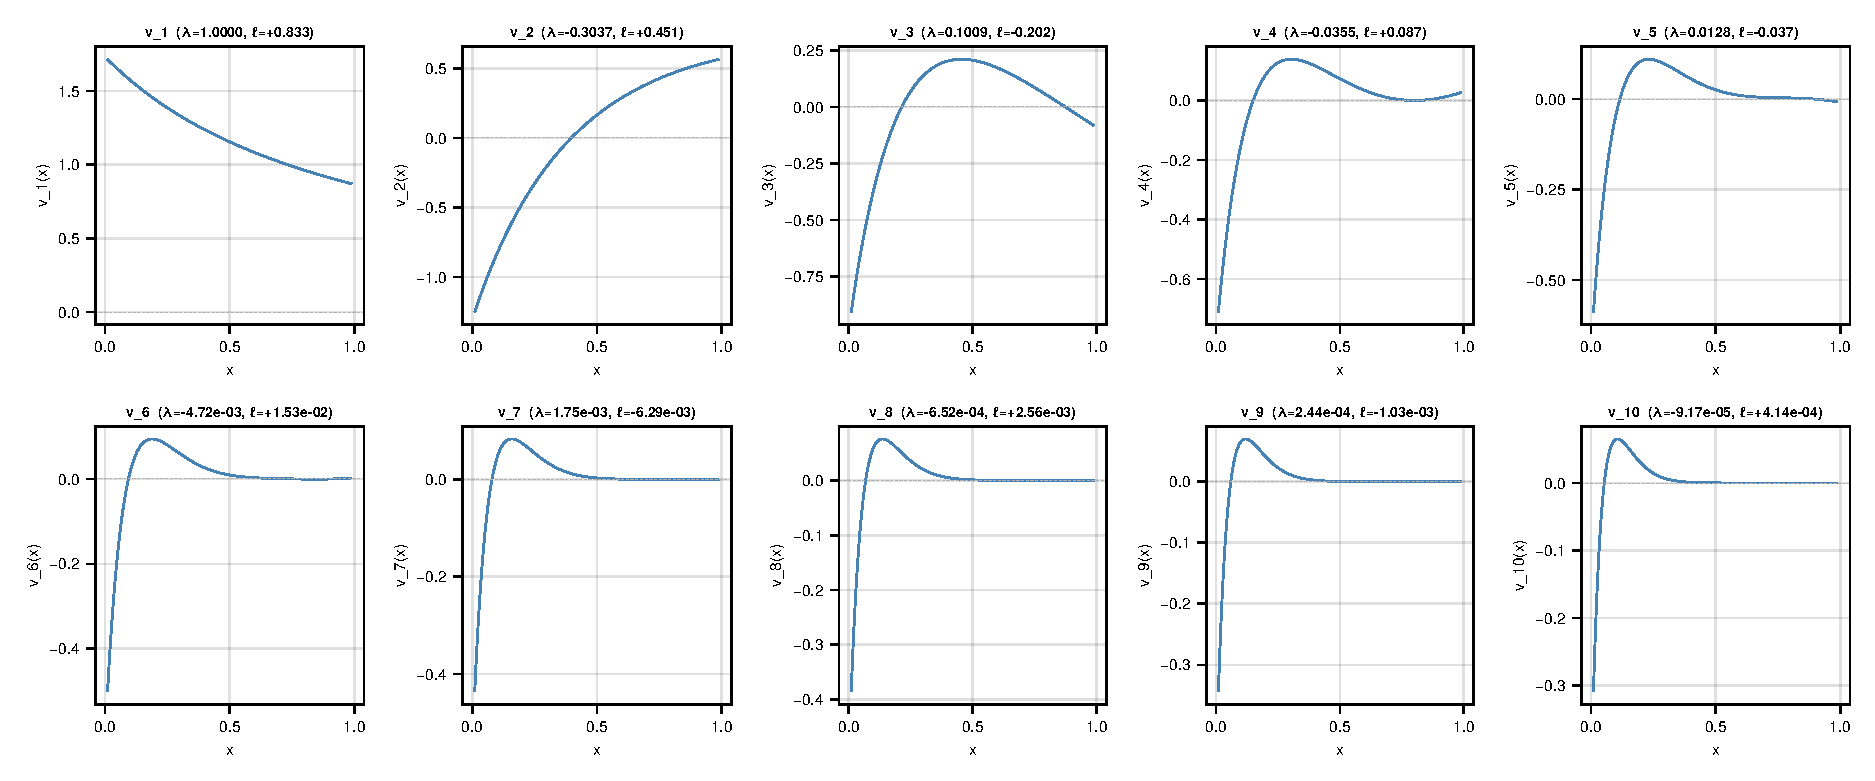
\includegraphics[width=\textwidth]{eigenfunctions_1_10.pdf}
\caption{Eigenfunctions $v_1, \ldots, v_{10}$. The invariant density $v_1$ (top left)
is positive; higher eigenfunctions oscillate with increasing frequency.
Each panel shows $\lambda_j$ and $\ell_j(\mathbf{1})$.}
\label{S-fig:eigenfunctions-1-10}
\end{figure}

\begin{figure}[ht]
\centering
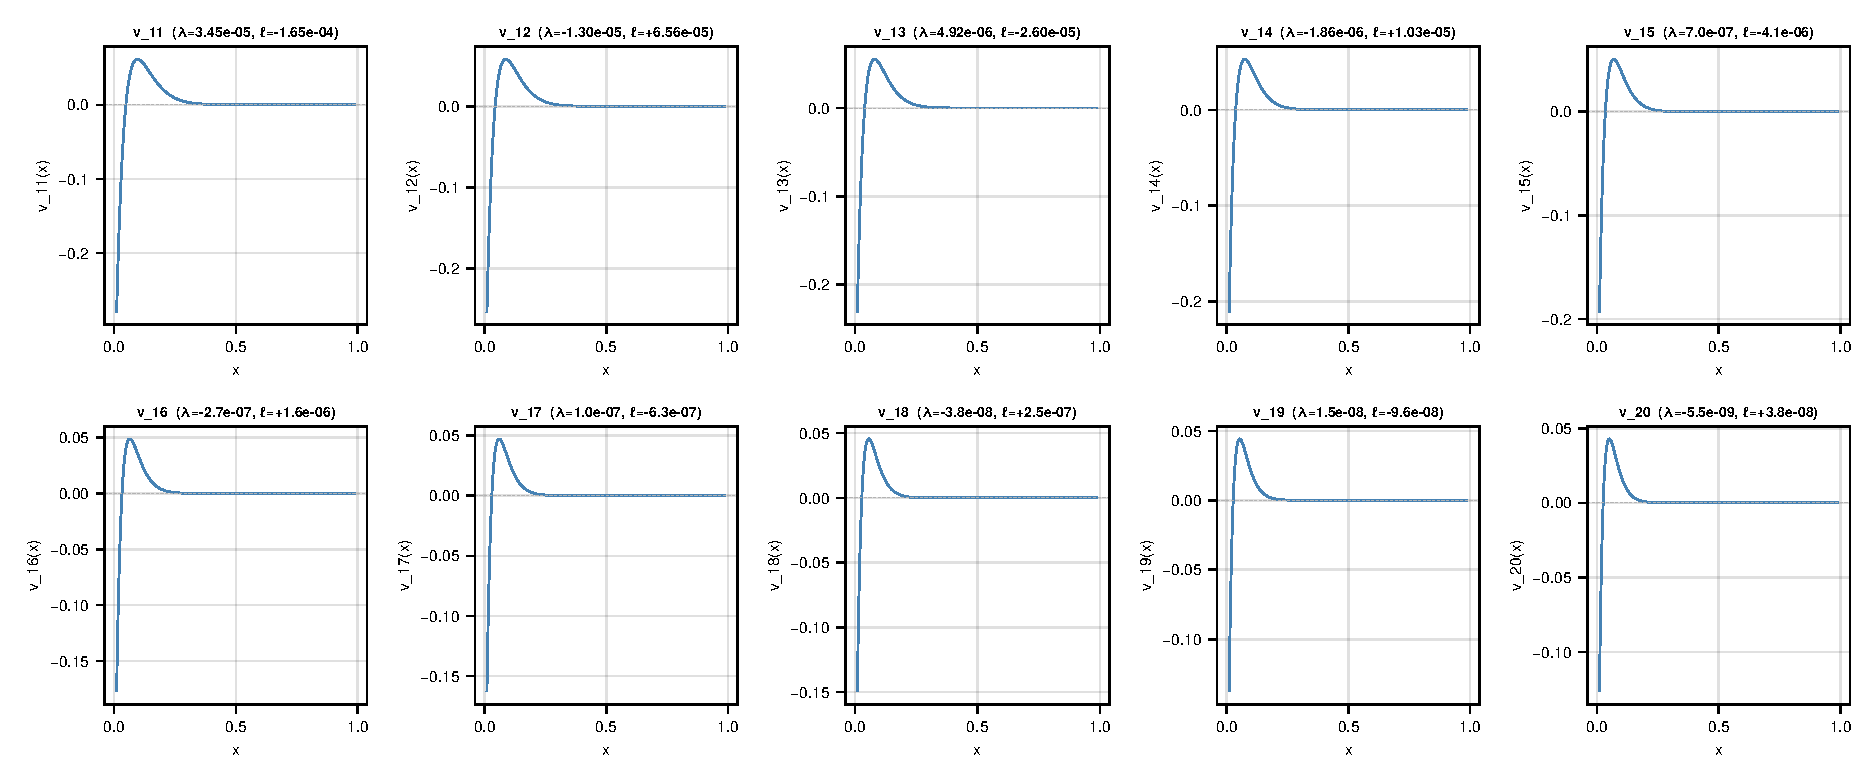
\includegraphics[width=\textwidth]{eigenfunctions_11_20.pdf}
\caption{Eigenfunctions $v_{11}, \ldots, v_{20}$.
Eigenvalues $|\lambda_j| \sim 10^{-5}$--$10^{-9}$;
these modes decay rapidly under iteration.}
\label{S-fig:eigenfunctions-11-20}
\end{figure}

\begin{figure}[ht]
\centering
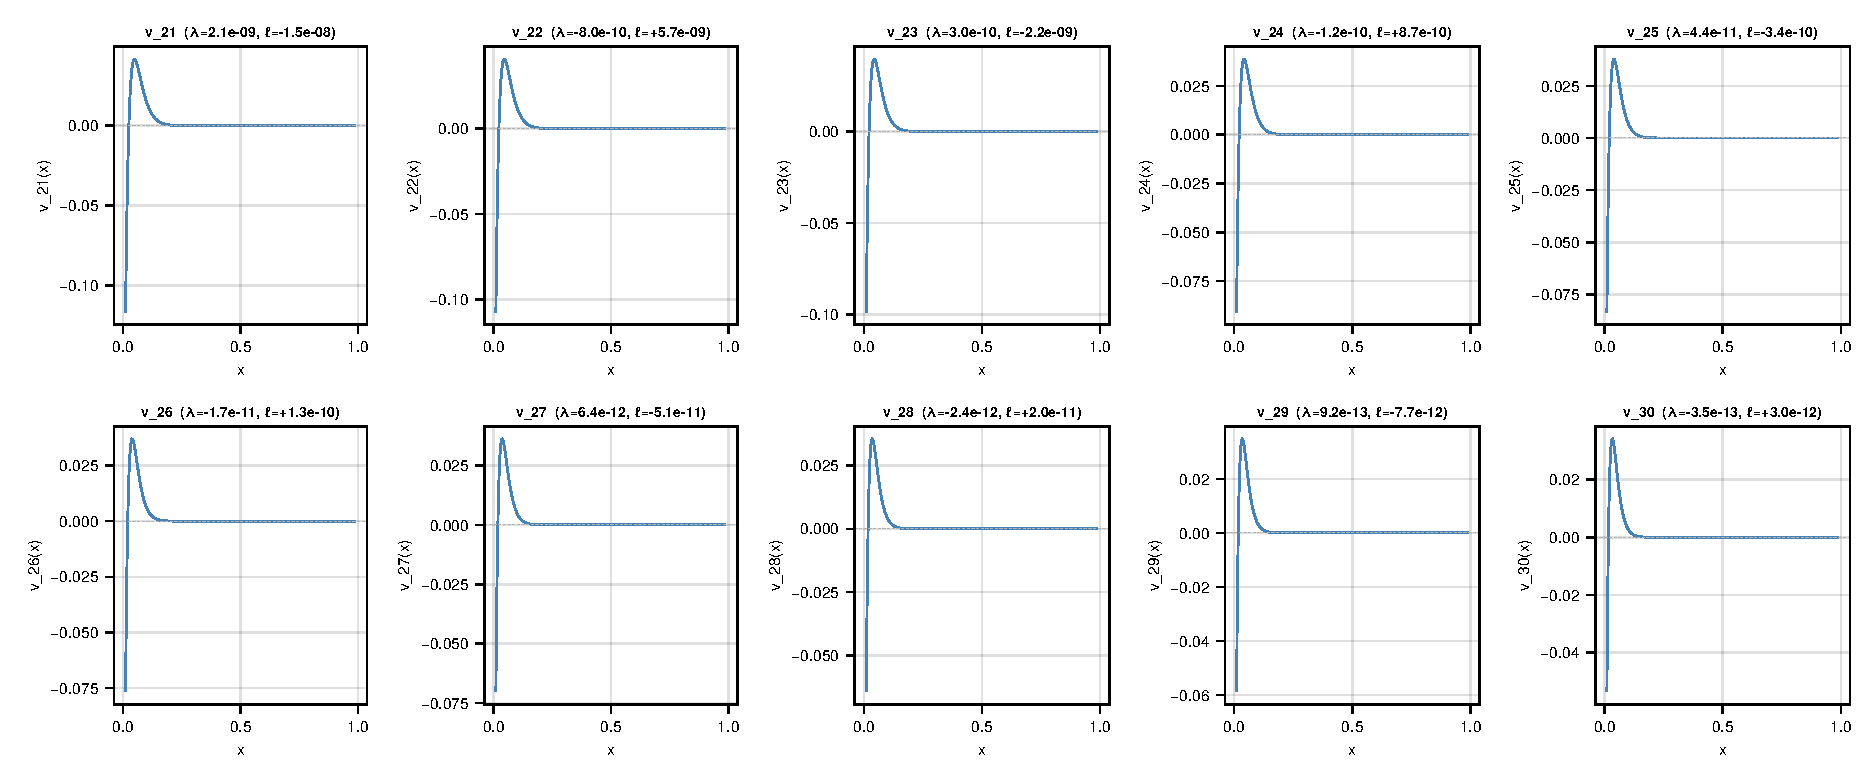
\includegraphics[width=\textwidth]{eigenfunctions_21_30.pdf}
\caption{Eigenfunctions $v_{21}, \ldots, v_{30}$.
Eigenvalues $|\lambda_j| \sim 10^{-9}$--$10^{-13}$.}
\label{S-fig:eigenfunctions-21-30}
\end{figure}

\begin{figure}[ht]
\centering
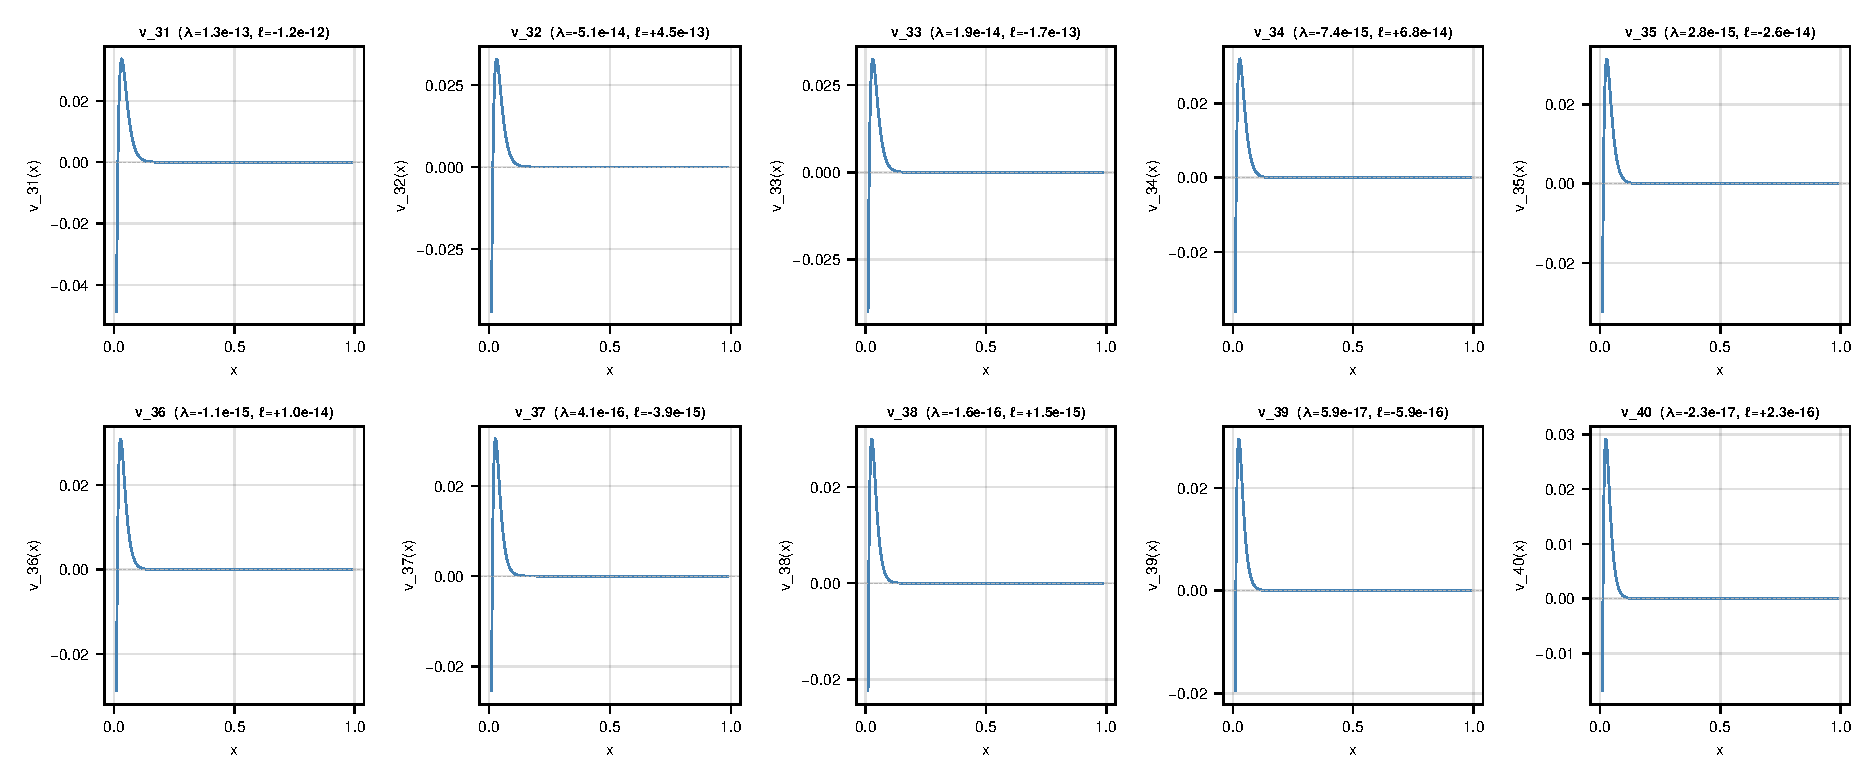
\includegraphics[width=\textwidth]{eigenfunctions_31_40.pdf}
\caption{Eigenfunctions $v_{31}, \ldots, v_{40}$.
Eigenvalues $|\lambda_j| \sim 10^{-13}$--$10^{-17}$.}
\label{S-fig:eigenfunctions-31-40}
\end{figure}

\begin{figure}[ht]
\centering
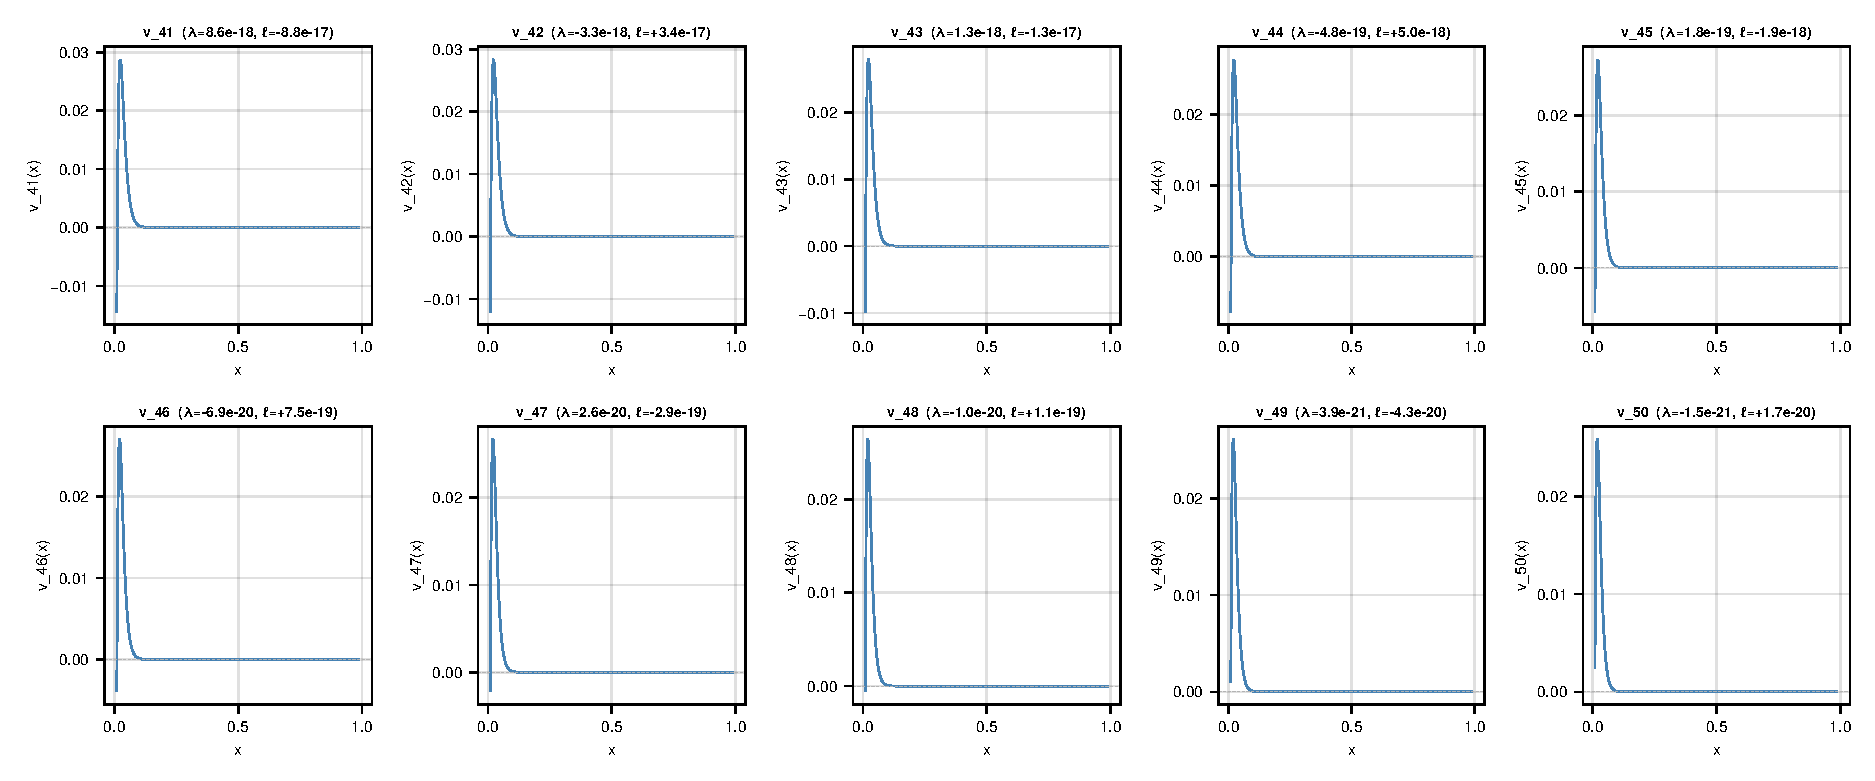
\includegraphics[width=\textwidth]{eigenfunctions_41_50.pdf}
\caption{Eigenfunctions $v_{41}, \ldots, v_{50}$.
Eigenvalues $|\lambda_j| \sim 10^{-17}$--$10^{-21}$.}
\label{S-fig:eigenfunctions-41-50}
\end{figure}

\begin{figure}[ht]
\centering
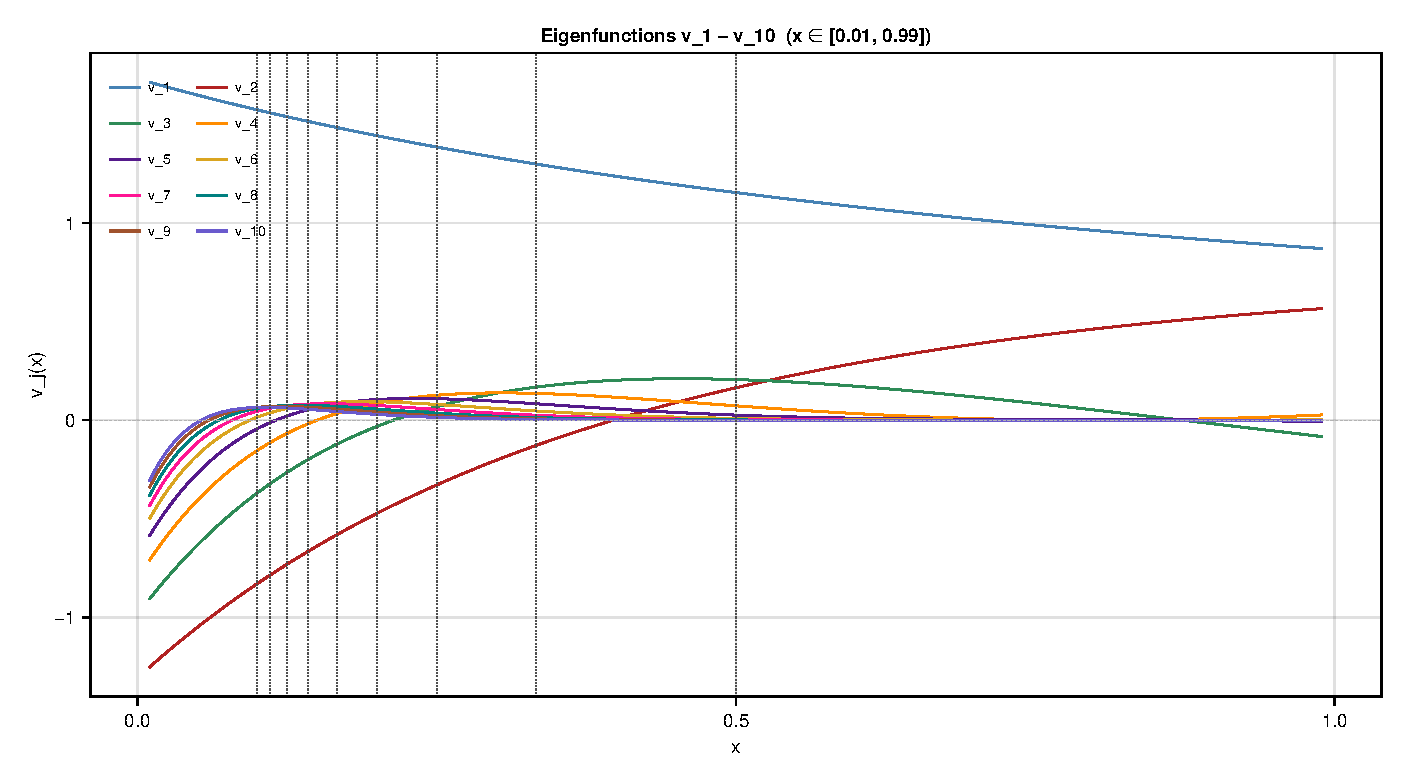
\includegraphics[width=0.85\textwidth]{eigenfunctions_1_10_overlay.pdf}
\caption{Eigenfunctions $v_1, \ldots, v_{10}$ overlaid with Markov partition
(vertical lines at $x = 1/n$, $n = 2, \ldots, 10$).}
\label{S-fig:eigenfunctions-1-10-overlay}
\end{figure}

\begin{figure}[ht]
\centering
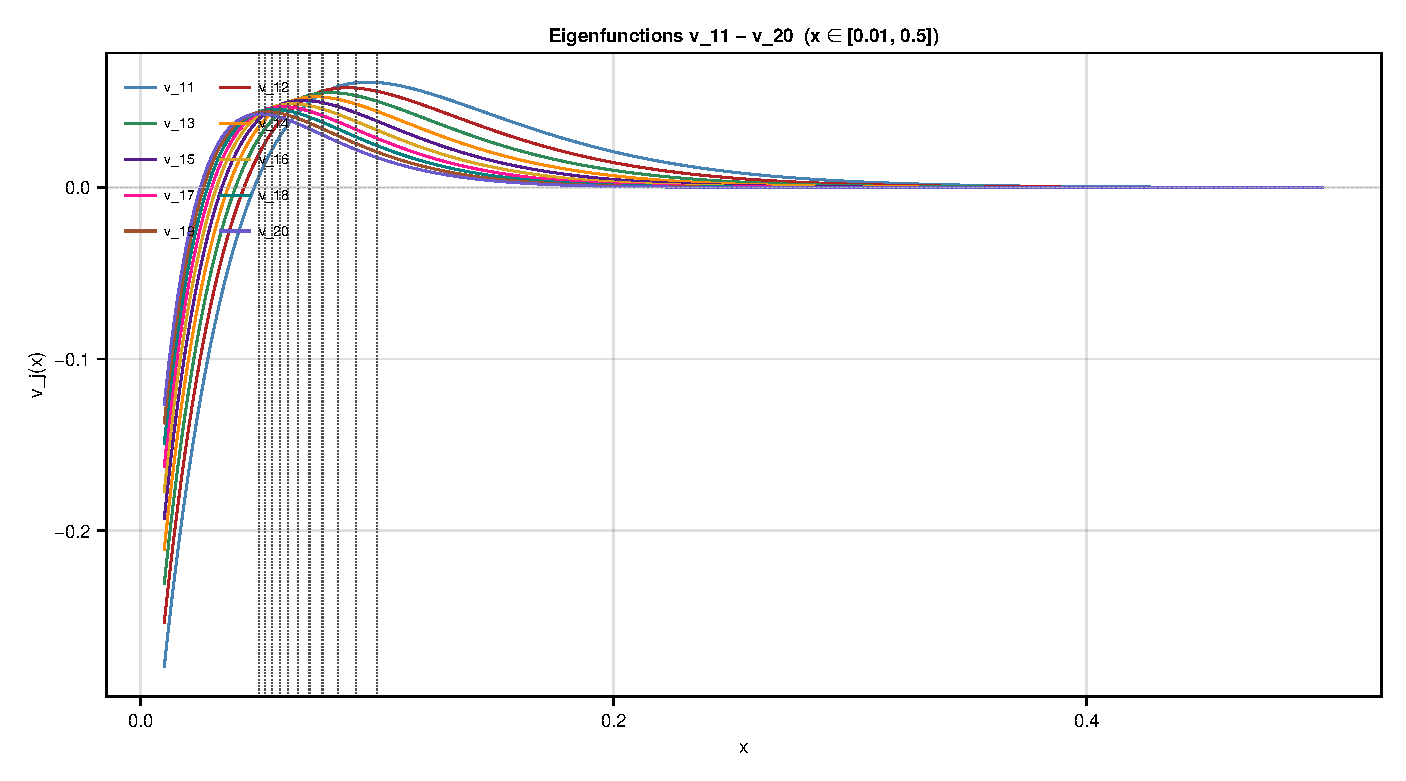
\includegraphics[width=0.85\textwidth]{eigenfunctions_11_20_overlay.pdf}
\caption{Eigenfunctions $v_{11}, \ldots, v_{20}$ overlaid with Markov partition.}
\label{S-fig:eigenfunctions-11-20-overlay}
\end{figure}

\begin{figure}[ht]
\centering
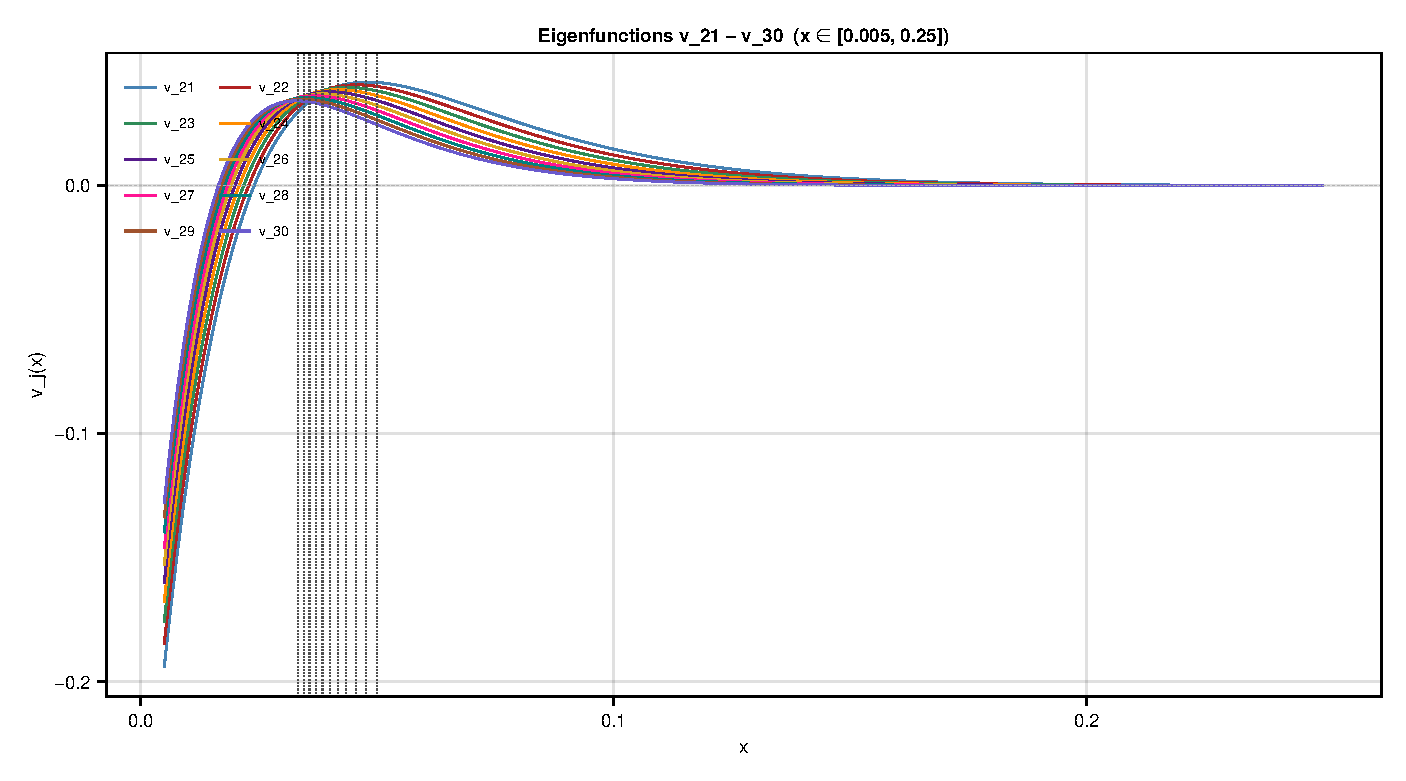
\includegraphics[width=0.85\textwidth]{eigenfunctions_21_30_overlay.pdf}
\caption{Eigenfunctions $v_{21}, \ldots, v_{30}$ overlaid with Markov partition.}
\label{S-fig:eigenfunctions-21-30-overlay}
\end{figure}

\begin{figure}[ht]
\centering
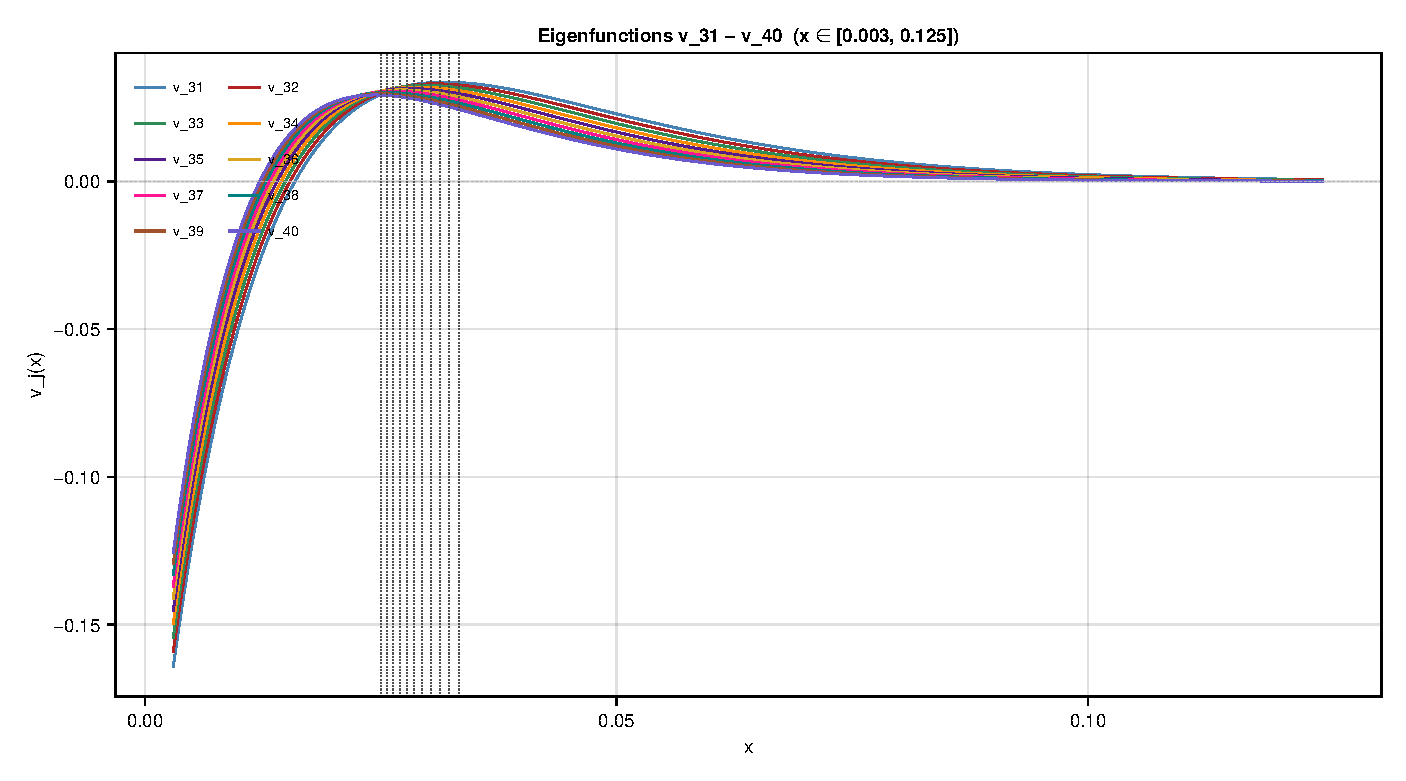
\includegraphics[width=0.85\textwidth]{eigenfunctions_31_40_overlay.pdf}
\caption{Eigenfunctions $v_{31}, \ldots, v_{40}$ overlaid with Markov partition.}
\label{S-fig:eigenfunctions-31-40-overlay}
\end{figure}

\begin{figure}[ht]
\centering
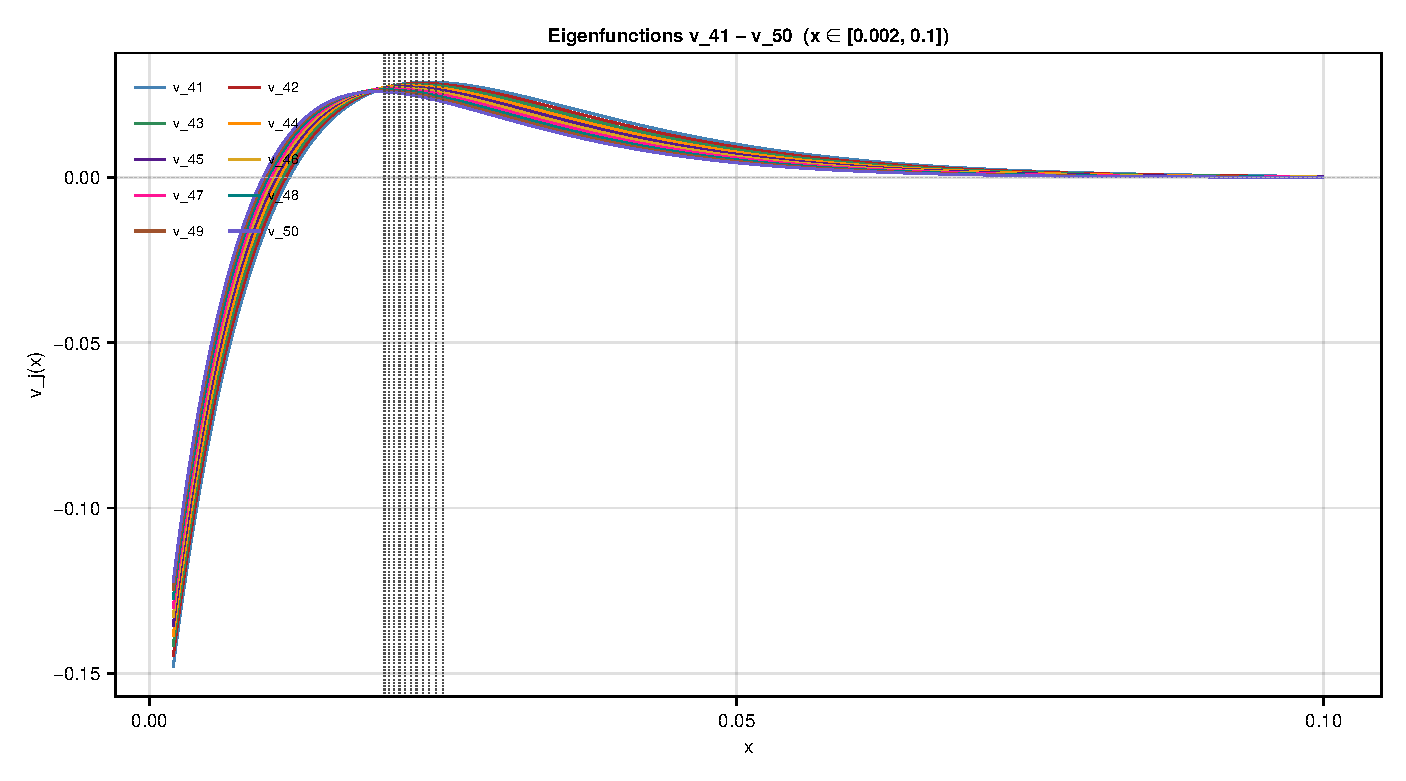
\includegraphics[width=0.85\textwidth]{eigenfunctions_41_50_overlay.pdf}
\caption{Eigenfunctions $v_{41}, \ldots, v_{50}$ overlaid with Markov partition.}
\label{S-fig:eigenfunctions-41-50-overlay}
\end{figure}

\begin{figure}[ht]
\centering
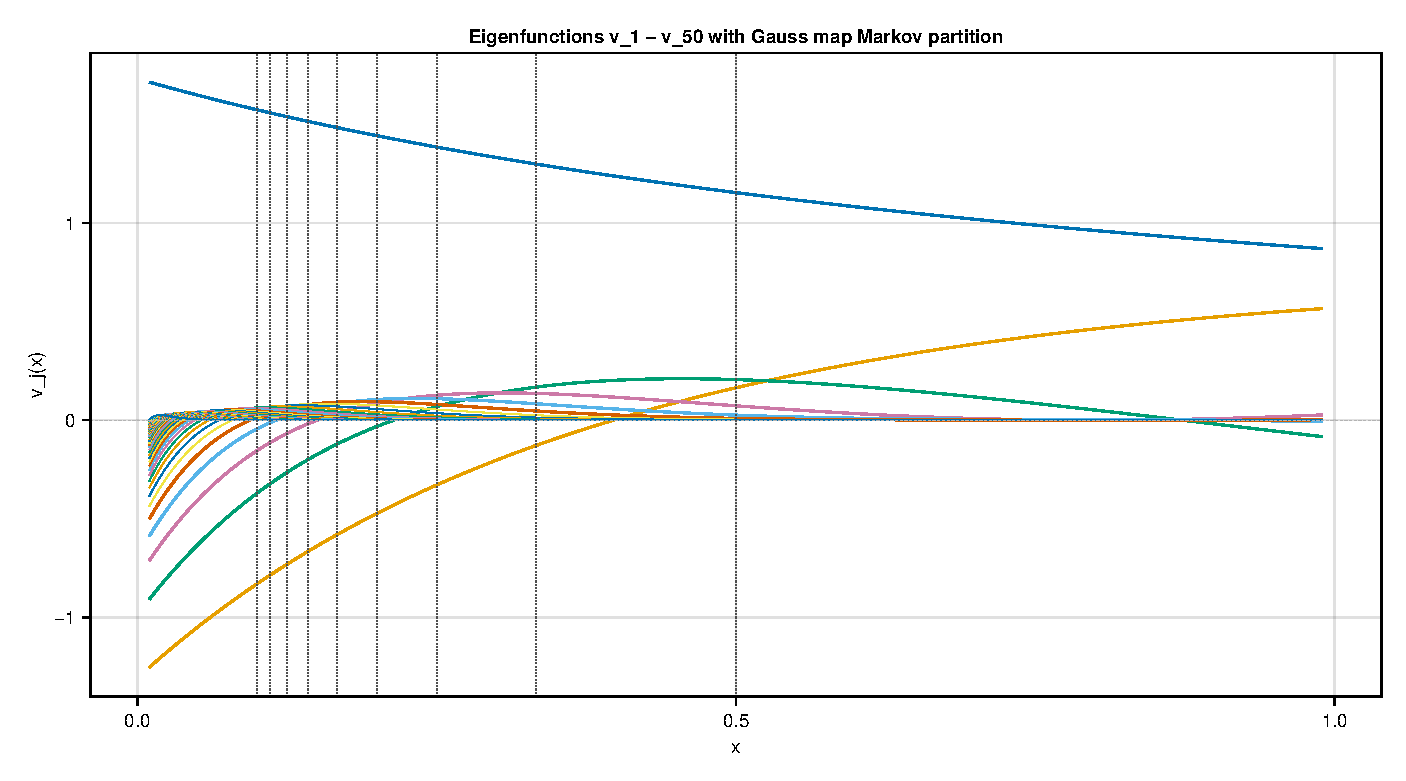
\includegraphics[width=0.85\textwidth]{eigenfunctions_all_overlay.pdf}
\caption{All $50$ eigenfunctions overlaid, with Gauss map Markov partition
(vertical dotted lines at $x = 1/n$, $n = 2, \ldots, 10$).}
\label{S-fig:eigenfunctions-all-overlay}
\end{figure}

\begin{figure}[ht]
\centering
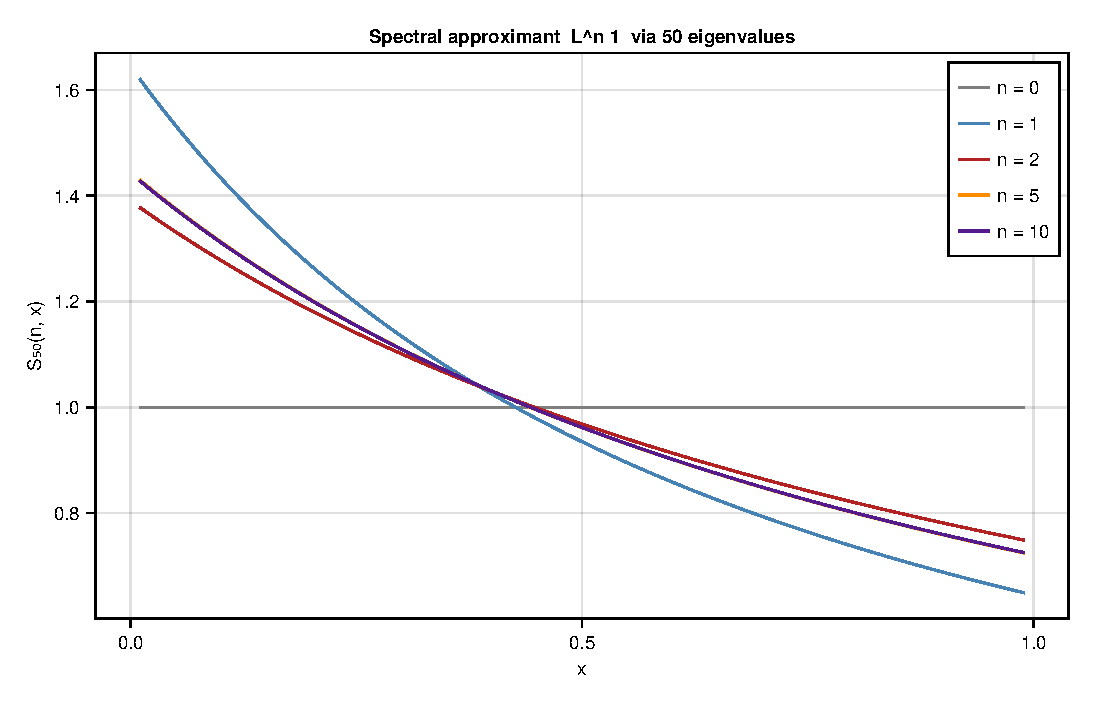
\includegraphics[width=0.85\textwidth]{spectral_approximant.pdf}
\caption{Spectral approximant $S_{50}(n, x) = \sum_{j=1}^{50} \lambda_j^n \, \ell_j(\mathbf{1}) \, v_j(x)$
for $n = 0, 1, 2, 5, 10$.  At $n = 0$ the sum reconstructs the constant function~$\mathbf{1}$;
at $n = 1$ it approximates the transfer operator applied to~$\mathbf{1}$;
for large~$n$ it converges to $\lambda_1^n \, \ell_1(\mathbf{1}) \, v_1(x)$.}
\label{S-fig:spectral-approximant}
\end{figure}

\begin{figure}[ht]
\centering
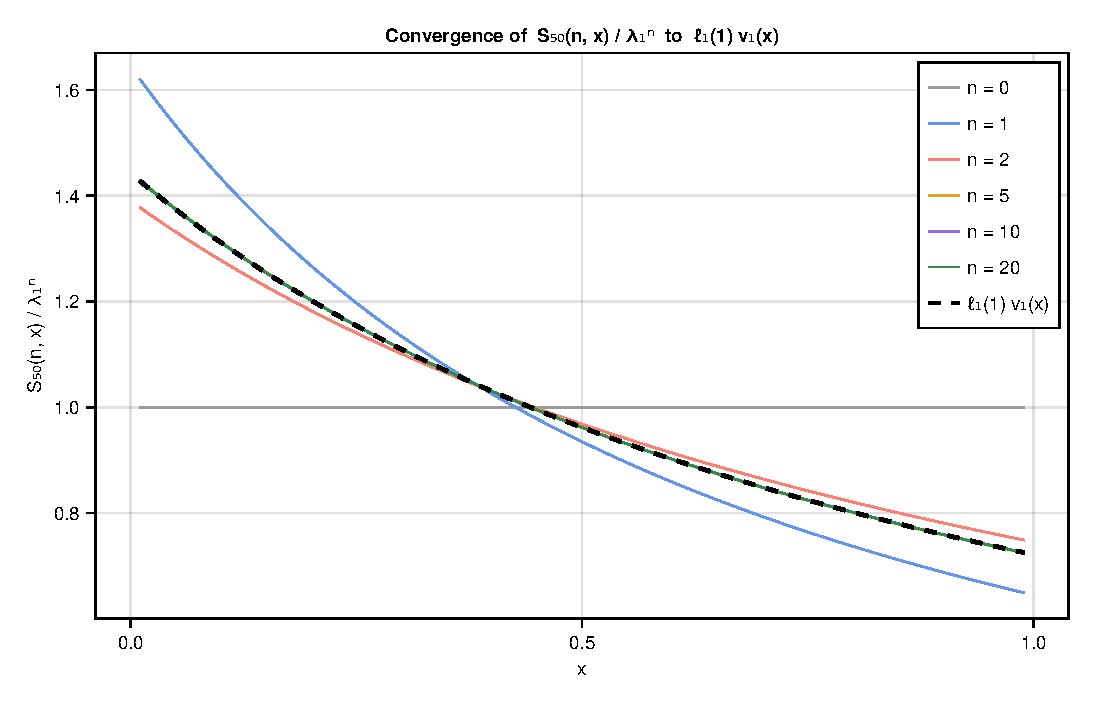
\includegraphics[width=0.85\textwidth]{spectral_convergence.pdf}
\caption{Convergence of $S_{50}(n, x) / \lambda_1^n$ to the invariant density
$\ell_1(\mathbf{1}) \, v_1(x)$ (dashed black).
The spectral gap $|\lambda_2 / \lambda_1| \approx 0.304$ governs the rate of convergence.}
\label{S-fig:spectral-convergence}
\end{figure}

\clearpage
\subsection*{Eigenvector Coefficients $[v_j]_k$}

The following tables list the first $50$ coefficients of each unit-norm
eigenvector $v_j$ in the shifted monomial basis $\{(w-1)^k\}_{k=0}^{K}$.
The $\ell^2$ error $\|\hat{v}_j - v_j\| \leq \delta_j$ shown for each
eigenvector is controlled by the Schur orthogonality defect and the
reconstruction error from the ordschur + Sylvester pipeline
(see Table~\ref{S-tab:spectral-data-K1024}).
Eigenvectors at $K = 1024$ (2048-bit precision) achieve radii $\sim 10^{-316}$--$10^{-282}$.

\paragraph{$j = 1$: $\lambda_{1} = 1.000000e+00$, \quad $\ell_{1}(\mathbf{1}) = +8.329404e-01$, \quad $\|\hat v_{1} - v_{1}\| \leq 3.62e-162$}
\begin{center}
{\footnotesize
\begin{tabular}{r@{\;\;}l@{\quad}r@{\;\;}l}
\toprule
$k$ & $[v_{1}]_k$ & $k$ & $[v_{1}]_k$ \\
\midrule
0 & $+8.6602540378e-01$ & 25 & $-2.5809568280e-08$ \\
1 & $-4.3301270189e-01$ & 26 & $+1.2904784140e-08$ \\
2 & $+2.1650635095e-01$ & 27 & $-6.4523920699e-09$ \\
3 & $-1.0825317547e-01$ & 28 & $+3.2261960349e-09$ \\
4 & $+5.4126587737e-02$ & 29 & $-1.6130980175e-09$ \\
5 & $-2.7063293868e-02$ & 30 & $+8.0654900873e-10$ \\
6 & $+1.3531646934e-02$ & 31 & $-4.0327450437e-10$ \\
7 & $-6.7658234671e-03$ & 32 & $+2.0163725218e-10$ \\
8 & $+3.3829117335e-03$ & 33 & $-1.0081862609e-10$ \\
9 & $-1.6914558668e-03$ & 34 & $+5.0409313046e-11$ \\
10 & $+8.4572793338e-04$ & 35 & $-2.5204656523e-11$ \\
11 & $-4.2286396669e-04$ & 36 & $+1.2602328261e-11$ \\
12 & $+2.1143198335e-04$ & 37 & $-6.3011641307e-12$ \\
13 & $-1.0571599167e-04$ & 38 & $+3.1505820654e-12$ \\
14 & $+5.2857995836e-05$ & 39 & $-1.5752910327e-12$ \\
15 & $-2.6428997918e-05$ & 40 & $+7.8764551634e-13$ \\
16 & $+1.3214498959e-05$ & 41 & $-3.9382275817e-13$ \\
17 & $-6.6072494796e-06$ & 42 & $+1.9691137909e-13$ \\
18 & $+3.3036247398e-06$ & 43 & $-9.8455689543e-14$ \\
19 & $-1.6518123699e-06$ & 44 & $+4.9227844771e-14$ \\
20 & $+8.2590618494e-07$ & 45 & $-2.4613922386e-14$ \\
21 & $-4.1295309247e-07$ & 46 & $+1.2306961193e-14$ \\
22 & $+2.0647654624e-07$ & 47 & $-6.1534805964e-15$ \\
23 & $-1.0323827312e-07$ & 48 & $+3.0767402982e-15$ \\
24 & $+5.1619136559e-08$ & 49 & $-1.5383701491e-15$ \\
\bottomrule
\end{tabular}
}
\end{center}

\paragraph{$j = 2$: $\lambda_{2} = -3.036630e-01$, \quad $\ell_{2}(\mathbf{1}) = +4.512058e-01$, \quad $\|\hat v_{2} - v_{2}\| \leq 2.00e-161$}
\begin{center}
{\footnotesize
\begin{tabular}{r@{\;\;}l@{\quad}r@{\;\;}l}
\toprule
$k$ & $[v_{2}]_k$ & $k$ & $[v_{2}]_k$ \\
\midrule
0 & $+5.7050920659e-01$ & 25 & $+2.1137822436e-07$ \\
1 & $+4.1624549960e-01$ & 26 & $-1.0569761625e-07$ \\
2 & $-5.1196167436e-01$ & 27 & $+5.2851197768e-08$ \\
3 & $+3.8491986254e-01$ & 28 & $-2.6426213142e-08$ \\
4 & $-2.4616997141e-01$ & 29 & $+1.3213239926e-08$ \\
5 & $+1.4508248976e-01$ & 30 & $-6.6066375954e-09$ \\
6 & $-8.1412161204e-02$ & 31 & $+3.3033150334e-09$ \\
7 & $+4.4232939695e-02$ & 32 & $-1.6516529702e-09$ \\
8 & $-2.3500357920e-02$ & 33 & $+8.2582392107e-10$ \\
9 & $+1.2286594354e-02$ & 34 & $-4.1291080660e-10$ \\
10 & $-6.3488447731e-03$ & 35 & $+2.0645495059e-10$ \\
11 & $+3.2523318873e-03$ & 36 & $-1.0322731864e-10$ \\
12 & $-1.6553890182e-03$ & 37 & $+5.1613613481e-11$ \\
13 & $+8.3854489512e-04$ & 38 & $-2.5806797425e-11$ \\
14 & $-4.2326095063e-04$ & 39 & $+1.2903399301e-11$ \\
15 & $+2.1308196815e-04$ & 40 & $-6.4517018099e-12$ \\
16 & $-1.0706384161e-04$ & 41 & $+3.2258525849e-12$ \\
17 & $+5.3718283692e-05$ & 42 & $-1.6129272967e-12$ \\
18 & $-2.6924831316e-05$ & 43 & $+8.0646418026e-13$ \\
19 & $+1.3485294563e-05$ & 44 & $-4.0323235203e-13$ \\
20 & $-6.7505119961e-06$ & 45 & $+2.0161629853e-13$ \\
21 & $+3.3779201786e-06$ & 46 & $-1.0080820435e-13$ \\
22 & $-1.6898475614e-06$ & 47 & $+5.0404126138e-14$ \\
23 & $+8.4521363390e-07$ & 48 & $-2.5202073187e-14$ \\
24 & $-4.2269924754e-07$ & 49 & $+1.2601040747e-14$ \\
\bottomrule
\end{tabular}
}
\end{center}

\paragraph{$j = 3$: $\lambda_{3} = 1.008845e-01$, \quad $\ell_{3}(\mathbf{1}) = -2.019399e-01$, \quad $\|\hat v_{3} - v_{3}\| \leq 9.37e-161$}
\begin{center}
{\footnotesize
\begin{tabular}{r@{\;\;}l@{\quad}r@{\;\;}l}
\toprule
$k$ & $[v_{3}]_k$ & $k$ & $[v_{3}]_k$ \\
\midrule
0 & $-9.0447344941e-02$ & 25 & $+1.4405034690e-06$ \\
1 & $-7.0686601071e-01$ & 26 & $-7.2111182399e-07$ \\
2 & $+9.4489856788e-02$ & 27 & $+3.6084832338e-07$ \\
3 & $+3.0867750376e-01$ & 28 & $-1.8052087863e-07$ \\
4 & $-4.0512541768e-01$ & 29 & $+9.0291304149e-08$ \\
5 & $+3.4761664596e-01$ & 30 & $-4.5155022432e-08$ \\
6 & $-2.4964571405e-01$ & 31 & $+2.2580145600e-08$ \\
7 & $+1.6202173376e-01$ & 32 & $-1.1290716982e-08$ \\
8 & $-9.8450913170e-02$ & 33 & $+5.6454685428e-09$ \\
9 & $+5.7125257848e-02$ & 34 & $-2.8227263359e-09$ \\
10 & $-3.2043727636e-02$ & 35 & $+1.4113422414e-09$ \\
11 & $+1.7521112776e-02$ & 36 & $-7.0565691808e-10$ \\
12 & $-9.3937359563e-03$ & 37 & $+3.5282096728e-10$ \\
13 & $+4.9597294662e-03$ & 38 & $-1.7640697401e-10$ \\
14 & $-2.5873265244e-03$ & 39 & $+8.8201962240e-11$ \\
15 & $+1.3369832382e-03$ & 40 & $-4.4100355916e-11$ \\
16 & $-6.8572831237e-04$ & 41 & $+2.2049934531e-11$ \\
17 & $+3.4963821569e-04$ & 42 & $-1.1024877405e-11$ \\
18 & $-1.7744974958e-04$ & 43 & $+5.5124075668e-12$ \\
19 & $+8.9734547254e-05$ & 44 & $-2.7561939091e-12$ \\
20 & $-4.5250271856e-05$ & 45 & $+1.3780942688e-12$ \\
21 & $+2.2768685168e-05$ & 46 & $-6.8904664447e-13$ \\
22 & $-1.1437476432e-05$ & 47 & $+3.4452338541e-13$ \\
23 & $+5.7381449931e-06$ & 48 & $-1.7226182909e-13$ \\
24 & $-2.8760584487e-06$ & 49 & $+8.6131015376e-14$ \\
\bottomrule
\end{tabular}
}
\end{center}

\paragraph{$j = 4$: $\lambda_{4} = -3.549616e-02$, \quad $\ell_{4}(\mathbf{1}) = +8.740239e-02$, \quad $\|\hat v_{4} - v_{4}\| \leq 3.83e-160$}
\begin{center}
{\footnotesize
\begin{tabular}{r@{\;\;}l@{\quad}r@{\;\;}l}
\toprule
$k$ & $[v_{4}]_k$ & $k$ & $[v_{4}]_k$ \\
\midrule
0 & $+2.9668451307e-02$ & 25 & $+9.3012438559e-06$ \\
1 & $+2.7924054265e-01$ & 26 & $-4.6825960255e-06$ \\
2 & $+5.6853860189e-01$ & 27 & $+2.3534773267e-06$ \\
3 & $-4.4824188327e-01$ & 28 & $-1.1813144791e-06$ \\
4 & $+3.3409474574e-02$ & 29 & $+5.9235060337e-07$ \\
5 & $+2.5167800897e-01$ & 30 & $-2.9679138185e-07$ \\
6 & $-3.4618786849e-01$ & 31 & $+1.4861544706e-07$ \\
7 & $+3.2023977666e-01$ & 32 & $-7.4384269422e-08$ \\
8 & $-2.4757279345e-01$ & 33 & $+3.7218012651e-08$ \\
9 & $+1.7190363582e-01$ & 34 & $-1.8617414047e-08$ \\
10 & $-1.1098770133e-01$ & 35 & $+9.3112868289e-09$ \\
11 & $+6.7973144203e-02$ & 36 & $-4.6563649096e-09$ \\
12 & $-3.9996876950e-02$ & 37 & $+2.3283501234e-09$ \\
13 & $+2.2812107298e-02$ & 38 & $-1.1641958726e-09$ \\
14 & $-1.2691930309e-02$ & 39 & $+5.8208892068e-10$ \\
15 & $+6.9215101502e-03$ & 40 & $-2.9103450369e-10$ \\
16 & $-3.7136745268e-03$ & 41 & $+1.4551100833e-10$ \\
17 & $+1.9661656212e-03$ & 42 & $-7.2752230647e-11$ \\
18 & $-1.0296382006e-03$ & 43 & $+3.6374552655e-11$ \\
19 & $+5.3437088712e-04$ & 44 & $-1.8186574860e-11$ \\
20 & $-2.7529049710e-04$ & 45 & $+9.0929869112e-12$ \\
21 & $+1.4096381725e-04$ & 46 & $-4.5463697302e-12$ \\
22 & $-7.1824532168e-05$ & 47 & $+2.2731358030e-12$ \\
23 & $+3.6449132229e-05$ & 48 & $-1.1365491915e-12$ \\
24 & $-1.8436745987e-05$ & 49 & $+5.6826777399e-13$ \\
\bottomrule
\end{tabular}
}
\end{center}

\paragraph{$j = 5$: $\lambda_{5} = 1.284379e-02$, \quad $\ell_{5}(\mathbf{1}) = -3.694616e-02$, \quad $\|\hat v_{5} - v_{5}\| \leq 1.45e-159$}
\begin{center}
{\footnotesize
\begin{tabular}{r@{\;\;}l@{\quad}r@{\;\;}l}
\toprule
$k$ & $[v_{5}]_k$ & $k$ & $[v_{5}]_k$ \\
\midrule
0 & $-8.8043043986e-03$ & 25 & $+5.6712684176e-05$ \\
1 & $-1.2821141655e-01$ & 26 & $-2.8984255395e-05$ \\
2 & $-4.0620172038e-01$ & 27 & $+1.4751250734e-05$ \\
3 & $-2.5046189333e-01$ & 28 & $-7.4813774835e-06$ \\
4 & $+5.3864569107e-01$ & 29 & $+3.7833678490e-06$ \\
5 & $-3.4385788333e-01$ & 30 & $-1.9087125191e-06$ \\
6 & $+1.7687881189e-02$ & 31 & $+9.6107039237e-07$ \\
7 & $+2.1476374450e-01$ & 32 & $-4.8314951109e-07$ \\
8 & $-3.0753683353e-01$ & 33 & $+2.4257905525e-07$ \\
9 & $+3.0005617346e-01$ & 34 & $-1.2166964329e-07$ \\
10 & $-2.4487939302e-01$ & 35 & $+6.0976298735e-08$ \\
11 & $+1.7911864358e-01$ & 36 & $-3.0539790507e-08$ \\
12 & $-1.2144537659e-01$ & 37 & $+1.5288308267e-08$ \\
13 & $+7.7837988391e-02$ & 38 & $-7.6505288082e-09$ \\
14 & $-4.7763889976e-02$ & 39 & $+3.8273865267e-09$ \\
15 & $+2.8311025326e-02$ & 40 & $-1.9143609935e-09$ \\
16 & $-1.6314781544e-02$ & 41 & $+9.5737228056e-10$ \\
17 & $+9.1859688538e-03$ & 42 & $-4.7873208370e-10$ \\
18 & $-5.0730711145e-03$ & 43 & $+2.3937206451e-10$ \\
19 & $+2.7565802706e-03$ & 44 & $-1.1968356974e-10$ \\
20 & $-1.4775041526e-03$ & 45 & $+5.9838916142e-11$ \\
21 & $+7.8281931439e-04$ & 46 & $-2.9917598054e-11$ \\
22 & $-4.1071277215e-04$ & 47 & $+1.4957792419e-11$ \\
23 & $+2.1370271470e-04$ & 48 & $-7.4783998741e-12$ \\
24 & $-1.1041605544e-04$ & 49 & $+3.7389693930e-12$ \\
\bottomrule
\end{tabular}
}
\end{center}

\paragraph{$j = 6$: $\lambda_{6} = -4.717778e-03$, \quad $\ell_{6}(\mathbf{1}) = +1.534795e-02$, \quad $\|\hat v_{6} - v_{6}\| \leq 5.27e-159$}
\begin{center}
{\footnotesize
\begin{tabular}{r@{\;\;}l@{\quad}r@{\;\;}l}
\toprule
$k$ & $[v_{6}]_k$ & $k$ & $[v_{6}]_k$ \\
\midrule
0 & $+2.9288005304e-03$ & 25 & $+3.1381308619e-04$ \\
1 & $+5.2713511483e-02$ & 26 & $-1.6480576749e-04$ \\
2 & $+2.5758421280e-01$ & 27 & $+8.5893432199e-05$ \\
3 & $+3.7733209909e-01$ & 28 & $-4.4471579252e-05$ \\
4 & $-8.7332643623e-02$ & 29 & $+2.2894637725e-05$ \\
5 & $-3.7954659177e-01$ & 30 & $-1.1728959324e-05$ \\
6 & $+4.8680576276e-01$ & 31 & $+5.9836173338e-06$ \\
7 & $-2.8921038250e-01$ & 32 & $-3.0416841901e-06$ \\
8 & $+1.4754988883e-02$ & 33 & $+1.5415053684e-06$ \\
9 & $+1.8736691367e-01$ & 34 & $-7.7922335306e-07$ \\
10 & $-2.7901534902e-01$ & 35 & $+3.9304657578e-07$ \\
11 & $+2.8413322669e-01$ & 36 & $-1.9790044778e-07$ \\
12 & $-2.4217035435e-01$ & 37 & $+9.9495772191e-08$ \\
13 & $+1.8484043104e-01$ & 38 & $-4.9961213509e-08$ \\
14 & $-1.3057138188e-01$ & 39 & $+2.5062840942e-08$ \\
15 & $+8.7022433528e-02$ & 40 & $-1.2562613434e-08$ \\
16 & $-5.5410631501e-02$ & 41 & $+6.2929196399e-09$ \\
17 & $+3.4005412572e-02$ & 42 & $-3.1506873855e-09$ \\
18 & $-2.0244519606e-02$ & 43 & $+1.5768401622e-09$ \\
19 & $+1.1749626794e-02$ & 44 & $-7.8893057108e-10$ \\
20 & $-6.6741449169e-03$ & 45 & $+3.9463051949e-10$ \\
21 & $+3.7221436445e-03$ & 46 & $-1.9736447204e-10$ \\
22 & $-2.0433607145e-03$ & 47 & $+9.8694741849e-11$ \\
23 & $+1.1066109468e-03$ & 48 & $-4.9349373601e-11$ \\
24 & $-5.9230063610e-04$ & 49 & $+2.4674256052e-11$ \\
\bottomrule
\end{tabular}
}
\end{center}

\paragraph{$j = 7$: $\lambda_{7} = 1.748675e-03$, \quad $\ell_{7}(\mathbf{1}) = -6.294980e-03$, \quad $\|\hat v_{7} - v_{7}\| \leq 1.87e-158$}
\begin{center}
{\footnotesize
\begin{tabular}{r@{\;\;}l@{\quad}r@{\;\;}l}
\toprule
$k$ & $[v_{7}]_k$ & $k$ & $[v_{7}]_k$ \\
\midrule
0 & $-9.8055287385e-04$ & 25 & $+1.5153807365e-03$ \\
1 & $-2.1860588173e-02$ & 26 & $-8.2791609363e-04$ \\
2 & $-1.3820176619e-01$ & 27 & $+4.4707439112e-04$ \\
3 & $-3.4256938976e-01$ & 28 & $-2.3895005724e-04$ \\
4 & $-1.9744018209e-01$ & 29 & $+1.2656057412e-04$ \\
5 & $+2.9440585261e-01$ & 30 & $-6.6499936385e-05$ \\
6 & $+8.8207678372e-02$ & 31 & $+3.4696854350e-05$ \\
7 & $-4.1415744698e-01$ & 32 & $-1.7991781746e-05$ \\
8 & $+4.4439275024e-01$ & 33 & $+9.2790396749e-06$ \\
9 & $-2.5719478485e-01$ & 34 & $-4.7629002568e-06$ \\
10 & $+1.7193970567e-02$ & 35 & $+2.4346886257e-06$ \\
11 & $+1.6505458952e-01$ & 36 & $-1.2400950839e-06$ \\
12 & $-2.5611455673e-01$ & 37 & $+6.2967608130e-07$ \\
13 & $+2.7071961776e-01$ & 38 & $-3.1887337166e-07$ \\
14 & $-2.3939660325e-01$ & 39 & $+1.6111110867e-07$ \\
15 & $+1.8947230843e-01$ & 40 & $-8.1243217250e-08$ \\
16 & $-1.3866088775e-01$ & 41 & $+4.0900992244e-08$ \\
17 & $+9.5628348606e-02$ & 42 & $-2.0562710360e-08$ \\
18 & $-6.2923782054e-02$ & 43 & $+1.0325871095e-08$ \\
19 & $+3.9847890015e-02$ & 44 & $-5.1803558743e-09$ \\
20 & $-2.4442242880e-02$ & 45 & $+2.5968910133e-09$ \\
21 & $+1.4593481152e-02$ & 46 & $-1.3009868701e-09$ \\
22 & $-8.5143110135e-03$ & 47 & $+6.5143531766e-10$ \\
23 & $+4.8694811257e-03$ & 48 & $-3.2605766464e-10$ \\
24 & $-2.7370962618e-03$ & 49 & $+1.6314741925e-10$ \\
\bottomrule
\end{tabular}
}
\end{center}

\paragraph{$j = 8$: $\lambda_{8} = -6.520209e-04$, \quad $\ell_{8}(\mathbf{1}) = +2.557421e-03$, \quad $\|\hat v_{8} - v_{8}\| \leq 6.54e-158$}
\begin{center}
{\footnotesize
\begin{tabular}{r@{\;\;}l@{\quad}r@{\;\;}l}
\toprule
$k$ & $[v_{8}]_k$ & $k$ & $[v_{8}]_k$ \\
\midrule
0 & $+3.3816038721e-04$ & 25 & $+6.2014947319e-03$ \\
1 & $+8.8712621469e-03$ & 26 & $-3.5661271091e-03$ \\
2 & $+7.0040265312e-02$ & 27 & $+2.0174580968e-03$ \\
3 & $+2.3725221109e-01$ & 28 & $-1.1249354472e-03$ \\
4 & $+3.2135236940e-01$ & 29 & $+6.1924650269e-04$ \\
5 & $-4.5408229903e-02$ & 30 & $-3.3699277531e-04$ \\
6 & $-2.9898964426e-01$ & 31 & $+1.8152382819e-04$ \\
7 & $+1.7562043210e-01$ & 32 & $-9.6889519810e-05$ \\
8 & $+1.8249405818e-01$ & 33 & $+5.1294747872e-05$ \\
9 & $-4.1882715750e-01$ & 34 & $-2.6958830190e-05$ \\
10 & $+4.1193080144e-01$ & 35 & $+1.4076757346e-05$ \\
11 & $-2.3751440328e-01$ & 36 & $-7.3077905994e-06$ \\
12 & $+2.2412015993e-02$ & 37 & $+3.7742513570e-06$ \\
13 & $+1.4574225898e-01$ & 38 & $-1.9403952820e-06$ \\
14 & $-2.3660112868e-01$ & 39 & $+9.9356040970e-07$ \\
15 & $+2.5882669856e-01$ & 40 & $-5.0693439770e-07$ \\
16 & $-2.3645950137e-01$ & 41 & $+2.5784095463e-07$ \\
17 & $+1.9320544604e-01$ & 42 & $-1.3078741619e-07$ \\
18 & $-1.4587027901e-01$ & 43 & $+6.6183319911e-08$ \\
19 & $+1.0370377154e-01$ & 44 & $-3.3422489643e-08$ \\
20 & $-7.0278596440e-02$ & 45 & $+1.6848507392e-08$ \\
21 & $+4.5790881619e-02$ & 46 & $-8.4806233509e-09$ \\
22 & $-2.8867930402e-02$ & 47 & $+4.2632096248e-09$ \\
23 & $+1.7694940545e-02$ & 48 & $-2.1407970004e-09$ \\
24 & $-1.0586583669e-02$ & 49 & $+1.0740409385e-09$ \\
\bottomrule
\end{tabular}
}
\end{center}

\paragraph{$j = 9$: $\lambda_{9} = 2.441315e-04$, \quad $\ell_{9}(\mathbf{1}) = -1.031415e-03$, \quad $\|\hat v_{9} - v_{9}\| \leq 2.28e-157$}
\begin{center}
{\footnotesize
\begin{tabular}{r@{\;\;}l@{\quad}r@{\;\;}l}
\toprule
$k$ & $[v_{9}]_k$ & $k$ & $[v_{9}]_k$ \\
\midrule
0 & $-1.1799547910e-04$ & 25 & $+2.1031142393e-02$ \\
1 & $-3.5825018552e-03$ & 26 & $-1.2881889170e-02$ \\
2 & $-3.3725281451e-02$ & 27 & $+7.7187224649e-03$ \\
3 & $-1.4603058030e-01$ & 28 & $-4.5360503861e-03$ \\
4 & $-2.9886824515e-01$ & 29 & $+2.6200998185e-03$ \\
5 & $-1.8545475471e-01$ & 30 & $-1.4902832301e-03$ \\
6 & $+2.3247141884e-01$ & 31 & $+8.3603637339e-04$ \\
7 & $+1.3477449923e-01$ & 32 & $-4.6322633391e-04$ \\
8 & $-2.8813177543e-01$ & 33 & $+2.5380915511e-04$ \\
9 & $+8.1173431804e-02$ & 34 & $-1.3767079278e-04$ \\
10 & $+2.3449479102e-01$ & 35 & $+7.3998208039e-05$ \\
11 & $-4.1289479127e-01$ & 36 & $-3.9448207702e-05$ \\
12 & $+3.8721655110e-01$ & 37 & $+2.0873984602e-05$ \\
13 & $-2.2531195759e-01$ & 38 & $-1.0971579021e-05$ \\
14 & $+2.9238457729e-02$ & 39 & $+5.7319787919e-06$ \\
15 & $+1.2834557148e-01$ & 40 & $-2.9783320709e-06$ \\
16 & $-2.1925984696e-01$ & 41 & $+1.5399771601e-06$ \\
17 & $+2.4787497215e-01$ & 42 & $-7.9277105056e-07$ \\
18 & $-2.3328565645e-01$ & 43 & $+4.0651382364e-07$ \\
19 & $+1.9615236620e-01$ & 44 & $-2.0772176822e-07$ \\
20 & $-1.5229855765e-01$ & 45 & $+1.0581266317e-07$ \\
21 & $+1.1127777959e-01$ & 46 & $-5.3752382090e-08$ \\
22 & $-7.7451963565e-02$ & 47 & $+2.7239826076e-08$ \\
23 & $+5.1792687547e-02$ & 48 & $-1.3774854450e-08$ \\
24 & $-3.3484691285e-02$ & 49 & $+6.9528595371e-09$ \\
\bottomrule
\end{tabular}
}
\end{center}

\paragraph{$j = 10$: $\lambda_{10} = -9.168908e-05$, \quad $\ell_{10}(\mathbf{1}) = +4.135796e-04$, \quad $\|\hat v_{10} - v_{10}\| \leq 7.92e-157$}
\begin{center}
{\footnotesize
\begin{tabular}{r@{\;\;}l@{\quad}r@{\;\;}l}
\toprule
$k$ & $[v_{10}]_k$ & $k$ & $[v_{10}]_k$ \\
\midrule
0 & $+4.1693739426e-05$ & 25 & $+5.7817303214e-02$ \\
1 & $+1.4356803898e-03$ & 26 & $-3.8259119809e-02$ \\
2 & $+1.5740329954e-02$ & 27 & $+2.4579824204e-02$ \\
3 & $+8.2688195017e-02$ & 28 & $-1.5389964310e-02$ \\
4 & $+2.2620743416e-01$ & 29 & $+9.4199704682e-03$ \\
5 & $+2.7822067868e-01$ & 30 & $-5.6509683529e-03$ \\
6 & $-1.1595749712e-02$ & 31 & $+3.3295927307e-03$ \\
7 & $-2.7851814217e-01$ & 32 & $-1.9304193851e-03$ \\
8 & $+8.6091010633e-02$ & 33 & $+1.1030468741e-03$ \\
9 & $+2.1705213403e-01$ & 34 & $-6.2204291906e-04$ \\
10 & $-2.4686942041e-01$ & 35 & $+3.4662663351e-04$ \\
11 & $+1.2443907115e-02$ & 36 & $-1.9106926089e-04$ \\
12 & $+2.6344547145e-01$ & 37 & $+1.0428689691e-04$ \\
13 & $-4.0329954443e-01$ & 38 & $-5.6410453631e-05$ \\
14 & $+3.6828131879e-01$ & 39 & $+3.0263944566e-05$ \\
15 & $-2.1796047790e-01$ & 40 & $-1.6115430604e-05$ \\
16 & $+3.7053787775e-02$ & 41 & $+8.5230739066e-06$ \\
17 & $+1.1225066617e-01$ & 42 & $-4.4797368267e-06$ \\
18 & $-2.0337663545e-01$ & 43 & $+2.3412819003e-06$ \\
19 & $+2.3750705199e-01$ & 44 & $-1.2173745951e-06$ \\
20 & $-2.2982635410e-01$ & 45 & $+6.3004499121e-07$ \\
21 & $+1.9838764906e-01$ & 46 & $-3.2470412192e-07$ \\
22 & $-1.5801420611e-01$ & 47 & $+1.6670588380e-07$ \\
23 & $+1.1837004459e-01$ & 48 & $-8.5295443546e-08$ \\
24 & $-8.4423852514e-02$ & 49 & $+4.3507605710e-08$ \\
\bottomrule
\end{tabular}
}
\end{center}

\paragraph{$j = 11$: $\lambda_{11} = 3.451655e-05$, \quad $\ell_{11}(\mathbf{1}) = -1.650674e-04$, \quad $\|\hat v_{11} - v_{11}\| \leq 2.75e-156$}
\begin{center}
{\footnotesize
\begin{tabular}{r@{\;\;}l@{\quad}r@{\;\;}l}
\toprule
$k$ & $[v_{11}]_k$ & $k$ & $[v_{11}]_k$ \\
\midrule
0 & $-1.4856799781e-05$ & 25 & $+1.2499432422e-01$ \\
1 & $-5.7278068075e-04$ & 26 & $-9.1176725084e-02$ \\
2 & $-7.1637694239e-03$ & 27 & $+6.3833249597e-02$ \\
3 & $-4.4295545512e-02$ & 28 & $-4.3160820203e-02$ \\
4 & $-1.5096183323e-01$ & 29 & $+2.8319491938e-02$ \\
5 & $-2.7188625823e-01$ & 30 & $-1.8099765605e-02$ \\
6 & $-1.6590624973e-01$ & 31 & $+1.1302670227e-02$ \\
7 & $+1.8096331602e-01$ & 32 & $-6.9136900348e-03$ \\
8 & $+1.7480530397e-01$ & 33 & $+4.1513164595e-03$ \\
9 & $-2.3703415193e-01$ & 34 & $-2.4513203810e-03$ \\
10 & $-2.7476522023e-02$ & 35 & $+1.4257279586e-03$ \\
11 & $+2.4654543560e-01$ & 36 & $-8.1788697947e-04$ \\
12 & $-2.0169921280e-01$ & 37 & $+4.6333704418e-04$ \\
13 & $-3.6539556280e-02$ & 38 & $-2.5948751235e-04$ \\
14 & $+2.7919354800e-01$ & 39 & $+1.4380411081e-04$ \\
15 & $-3.9276889886e-01$ & 40 & $-7.8929597375e-05$ \\
16 & $+3.5365056420e-01$ & 41 & $+4.2940323581e-05$ \\
17 & $-2.1390123647e-01$ & 42 & $-2.3171830528e-05$ \\
18 & $+4.5494057165e-02$ & 43 & $+1.2411133618e-05$ \\
19 & $+9.7086078846e-02$ & 44 & $-6.6021004011e-06$ \\
20 & $-1.8850600773e-01$ & 45 & $+3.4899210672e-06$ \\
21 & $+2.2749255813e-01$ & 46 & $-1.8341597179e-06$ \\
22 & $-2.2605014548e-01$ & 47 & $+9.5886160127e-07$ \\
23 & $+1.9996431926e-01$ & 48 & $-4.9884607996e-07$ \\
24 & $-1.6306691331e-01$ & 49 & $+2.5837498578e-07$ \\
\bottomrule
\end{tabular}
}
\end{center}

\paragraph{$j = 12$: $\lambda_{12} = -1.301770e-05$, \quad $\ell_{12}(\mathbf{1}) = +6.562912e-05$, \quad $\|\hat v_{12} - v_{12}\| \leq 9.56e-156$}
\begin{center}
{\footnotesize
\begin{tabular}{r@{\;\;}l@{\quad}r@{\;\;}l}
\toprule
$k$ & $[v_{12}]_k$ & $k$ & $[v_{12}]_k$ \\
\midrule
0 & $+5.3326453385e-06$ & 25 & $+2.0092202477e-01$ \\
1 & $+2.2756510459e-04$ & 26 & $-1.6749389819e-01$ \\
2 & $+3.1994533880e-03$ & 27 & $+1.3116023367e-01$ \\
3 & $+2.2749944884e-02$ & 28 & $-9.7694842398e-02$ \\
4 & $+9.2766484638e-02$ & 29 & $+6.9812509799e-02$ \\
5 & $+2.1767285817e-01$ & 30 & $-4.8161849885e-02$ \\
6 & $+2.4906057084e-01$ & 31 & $+3.2229384441e-02$ \\
7 & $-7.2880184724e-04$ & 32 & $-2.0999682746e-02$ \\
8 & $-2.4549995292e-01$ & 33 & $+1.3363109696e-02$ \\
9 & $+1.0393677854e-02$ & 34 & $-8.3258752603e-03$ \\
10 & $+2.4310591520e-01$ & 35 & $+5.0897912214e-03$ \\
11 & $-1.6179713004e-01$ & 36 & $-3.0584633835e-03$ \\
12 & $-1.0323446777e-01$ & 37 & $+1.8093342105e-03$ \\
13 & $+2.4991258343e-01$ & 38 & $-1.0552116256e-03$ \\
14 & $-1.6088907999e-01$ & 39 & $+6.0741917329e-04$ \\
15 & $-7.1245282290e-02$ & 40 & $-3.4548596264e-04$ \\
16 & $+2.8705639065e-01$ & 41 & $+1.9434865776e-04$ \\
17 & $-3.8240024962e-01$ & 42 & $-1.0822239296e-04$ \\
18 & $+3.4224992398e-01$ & 43 & $+5.9700425540e-05$ \\
19 & $-2.1214532203e-01$ & 44 & $-3.2649208842e-05$ \\
20 & $+5.4328744753e-02$ & 45 & $+1.7712794772e-05$ \\
21 & $+8.2615459497e-02$ & 46 & $-9.5385491956e-06$ \\
22 & $-1.7435718831e-01$ & 47 & $+5.1015259849e-06$ \\
23 & $+2.1767791278e-01$ & 48 & $-2.7112190900e-06$ \\
24 & $-2.2193728096e-01$ & 49 & $+1.4324663259e-06$ \\
\bottomrule
\end{tabular}
}
\end{center}

\paragraph{$j = 13$: $\lambda_{13} = 4.916782e-06$, \quad $\ell_{13}(\mathbf{1}) = -2.600972e-05$, \quad $\|\hat v_{13} - v_{13}\| \leq 3.33e-155$}
\begin{center}
{\footnotesize
\begin{tabular}{r@{\;\;}l@{\quad}r@{\;\;}l}
\toprule
$k$ & $[v_{13}]_k$ & $k$ & $[v_{13}]_k$ \\
\midrule
0 & $-1.9251350393e-06$ & 25 & $+2.0795837756e-01$ \\
1 & $-9.0120688193e-05$ & 26 & $-2.1747612414e-01$ \\
2 & $-1.4071545989e-03$ & 27 & $+2.0129170113e-01$ \\
3 & $-1.1313434202e-02$ & 28 & $-1.7132377568e-01$ \\
4 & $-5.3659908959e-02$ & 29 & $+1.3687437652e-01$ \\
5 & $-1.5458581942e-01$ & 30 & $-1.0396376707e-01$ \\
6 & $-2.5163194528e-01$ & 31 & $+7.5729727003e-02$ \\
7 & $-1.5007440271e-01$ & 32 & $-5.3236245942e-02$ \\
8 & $+1.5241951743e-01$ & 33 & $+3.6289385302e-02$ \\
9 & $+1.8094865039e-01$ & 34 & $-2.4077661904e-02$ \\
10 & $-1.7192716230e-01$ & 35 & $+1.5596595759e-02$ \\
11 & $-1.1489889704e-01$ & 36 & $-9.8881452546e-03$ \\
12 & $+2.4557237593e-01$ & 37 & $+6.1487178908e-03$ \\
13 & $-8.8591648220e-02$ & 38 & $-3.7568145553e-03$ \\
14 & $-1.5055178898e-01$ & 39 & $+2.2588886915e-03$ \\
15 & $+2.4112491343e-01$ & 40 & $-1.3384391950e-03$ \\
16 & $-1.2648307898e-01$ & 41 & $+7.8243844468e-04$ \\
17 & $-9.5709446764e-02$ & 42 & $-4.5176295674e-04$ \\
18 & $+2.9004328791e-01$ & 43 & $+2.5786523736e-04$ \\
19 & $-3.7260755967e-01$ & 44 & $-1.4563600466e-04$ \\
20 & $+3.3329298229e-01$ & 45 & $+8.1447123843e-05$ \\
21 & $-2.1203246136e-01$ & 46 & $-4.5135807056e-05$ \\
22 & $+6.3402917487e-02$ & 47 & $+2.4802003361e-05$ \\
23 & $+6.8682907158e-02$ & 48 & $-1.3521708824e-05$ \\
24 & $-1.6073398510e-01$ & 49 & $+7.3180468444e-06$ \\
\bottomrule
\end{tabular}
}
\end{center}

\paragraph{$j = 14$: $\lambda_{14} = -1.859307e-06$, \quad $\ell_{14}(\mathbf{1}) = +1.027988e-05$, \quad $\|\hat v_{14} - v_{14}\| \leq 1.16e-154$}
\begin{center}
{\footnotesize
\begin{tabular}{r@{\;\;}l@{\quad}r@{\;\;}l}
\toprule
$k$ & $[v_{14}]_k$ & $k$ & $[v_{14}]_k$ \\
\midrule
0 & $+6.9839204447e-07$ & 25 & $+5.5183102296e-02$ \\
1 & $+3.5590437909e-05$ & 26 & $-1.4750093339e-01$ \\
2 & $+6.1120610499e-04$ & 27 & $+1.9826164119e-01$ \\
3 & $+5.4824014243e-03$ & 28 & $-2.1266086666e-01$ \\
4 & $+2.9643512430e-02$ & 29 & $+2.0109845198e-01$ \\
5 & $+1.0100817539e-01$ & 30 & $-1.7457909549e-01$ \\
6 & $+2.1089546142e-01$ & 31 & $+1.4214115435e-01$ \\
7 & $+2.2613606565e-01$ & 32 & $-1.0997004731e-01$ \\
8 & $+3.8586220423e-03$ & 33 & $+8.1561628605e-02$ \\
9 & $-2.2222524508e-01$ & 34 & $-5.8359654245e-02$ \\
10 & $-2.8641204973e-02$ & 35 & $+4.0479930522e-02$ \\
11 & $+2.2532854208e-01$ & 36 & $-2.7321283018e-02$ \\
12 & $-6.5066300773e-02$ & 37 & $+1.7997574694e-02$ \\
13 & $-1.8658213373e-01$ & 38 & $-1.1600170958e-02$ \\
14 & $+2.1834492290e-01$ & 39 & $+7.3310127987e-03$ \\
15 & $-2.7552311101e-02$ & 40 & $-4.5508207970e-03$ \\
16 & $-1.7861462258e-01$ & 41 & $+2.7791521272e-03$ \\
17 & $+2.2733026157e-01$ & 42 & $-1.6719256136e-03$ \\
18 & $-9.8399813265e-02$ & 43 & $+9.9201702611e-04$ \\
19 & $-1.1276964385e-01$ & 44 & $-5.8113457693e-04$ \\
20 & $+2.8992422252e-01$ & 45 & $+3.3643364330e-04$ \\
21 & $-3.6350594136e-01$ & 46 & $-1.9264434256e-04$ \\
22 & $+3.2619624408e-01$ & 47 & $+1.0918968937e-04$ \\
23 & $-2.1310346976e-01$ & 48 & $-6.1302784273e-05$ \\
24 & $+7.2607085163e-02$ & 49 & $+3.4113866789e-05$ \\
\bottomrule
\end{tabular}
}
\end{center}

\paragraph{$j = 15$: $\lambda_{15} = 7.038113e-07$, \quad $\ell_{15}(\mathbf{1}) = -4.053403e-06$, \quad $\|\hat v_{15} - v_{15}\| \leq 4.03e-154$}
\begin{center}
{\footnotesize
\begin{tabular}{r@{\;\;}l@{\quad}r@{\;\;}l}
\toprule
$k$ & $[v_{15}]_k$ & $k$ & $[v_{15}]_k$ \\
\midrule
0 & $-2.5440017920e-07$ & 25 & $-2.1502807213e-01$ \\
1 & $-1.4022477968e-05$ & 26 & $+8.1860360750e-02$ \\
2 & $-2.6272062088e-04$ & 27 & $+4.2043984978e-02$ \\
3 & $-2.6012069807e-03$ & 28 & $-1.3456317163e-01$ \\
4 & $-1.5788943361e-02$ & 29 & $+1.8853772795e-01$ \\
5 & $-6.2043814076e-02$ & 30 & $-2.0749004043e-01$ \\
6 & $-1.5722370765e-01$ & 31 & $+2.0036342236e-01$ \\
7 & $-2.3565390879e-01$ & 32 & $-1.7727808525e-01$ \\
8 & $-1.3561427070e-01$ & 33 & $+1.4696337733e-01$ \\
9 & $+1.3325448741e-01$ & 34 & $-1.1570102844e-01$ \\
10 & $+1.8086453250e-01$ & 35 & $+8.7286618375e-02$ \\
11 & $-1.2714887956e-01$ & 36 & $-6.3509047340e-02$ \\
12 & $-1.5026485342e-01$ & 37 & $+4.4781927369e-02$ \\
13 & $+1.9297368195e-01$ & 38 & $-3.0717812120e-02$ \\
14 & $+2.9309212784e-02$ & 39 & $+2.0559725140e-02$ \\
15 & $-2.1910446217e-01$ & 40 & $-1.3460745442e-02$ \\
16 & $+1.8071658077e-01$ & 41 & $+8.6388384265e-03$ \\
17 & $+2.0239796958e-02$ & 42 & $-5.4444040770e-03$ \\
18 & $-1.9415530102e-01$ & 43 & $+3.3745964472e-03$ \\
19 & $+2.1214228010e-01$ & 44 & $-2.0599280735e-03$ \\
20 & $-7.5900765837e-02$ & 45 & $+1.2398053912e-03$ \\
21 & $-1.2440590241e-01$ & 46 & $-7.3651436339e-04$ \\
22 & $+2.8777318166e-01$ & 47 & $+4.3225702156e-04$ \\
23 & $-3.5507923797e-01$ & 48 & $-2.5084320874e-04$ \\
24 & $+3.2051989679e-01$ & 49 & $+1.4404356517e-04$ \\
\bottomrule
\end{tabular}
}
\end{center}

\paragraph{$j = 16$: $\lambda_{16} = -2.666413e-07$, \quad $\ell_{16}(\mathbf{1}) = +1.595012e-06$, \quad $\|\hat v_{16} - v_{16}\| \leq 1.41e-153$}
\begin{center}
{\footnotesize
\begin{tabular}{r@{\;\;}l@{\quad}r@{\;\;}l}
\toprule
$k$ & $[v_{16}]_k$ & $k$ & $[v_{16}]_k$ \\
\midrule
0 & $+9.2996230395e-08$ & 25 & $-3.4725646475e-01$ \\
1 & $+5.5135688933e-06$ & 26 & $+3.1592718589e-01$ \\
2 & $+1.1193313080e-04$ & 27 & $-2.1756182882e-01$ \\
3 & $+1.2126129608e-03$ & 28 & $+9.1100549291e-02$ \\
4 & $+8.1636033175e-03$ & 29 & $+2.9216186478e-02$ \\
5 & $+3.6316728617e-02$ & 30 & $-1.2185392133e-01$ \\
6 & $+1.0792745979e-01$ & 31 & $+1.7875253842e-01$ \\
7 & $+2.0505505174e-01$ & 32 & $-2.0196552123e-01$ \\
8 & $+2.0743349642e-01$ & 33 & $+1.9910506297e-01$ \\
9 & $+4.1733275532e-03$ & 34 & $-1.7943588558e-01$ \\
10 & $-2.0334560247e-01$ & 35 & $+1.5134273703e-01$ \\
11 & $-5.3398498140e-02$ & 36 & $-1.2114474722e-01$ \\
12 & $+2.0454995644e-01$ & 37 & $+9.2884488580e-02$ \\
13 & $-2.7238319182e-03$ & 38 & $-6.8662512632e-02$ \\
14 & $-2.0186731146e-01$ & 39 & $+4.9176688427e-02$ \\
15 & $+1.3107653491e-01$ & 40 & $-3.4254239815e-02$ \\
16 & $+9.9945226519e-02$ & 41 & $+2.3276032422e-02$ \\
17 & $-2.2698787815e-01$ & 42 & $-1.5467844597e-02$ \\
18 & $+1.4199152968e-01$ & 43 & $+1.0073630785e-02$ \\
19 & $+5.6508088239e-02$ & 44 & $-6.4409576907e-03$ \\
20 & $-2.0172377992e-01$ & 45 & $+4.0493818697e-03$ \\
21 & $+1.9734367649e-01$ & 46 & $-2.5065755768e-03$ \\
22 & $-5.8123606009e-02$ & 47 & $+1.5294552637e-03$ \\
23 & $-1.3200862239e-01$ & 48 & $-9.2089308034e-04$ \\
24 & $+2.8425834978e-01$ & 49 & $+5.4764936320e-04$ \\
\bottomrule
\end{tabular}
}
\end{center}

\paragraph{$j = 17$: $\lambda_{17} = 1.010906e-07$, \quad $\ell_{17}(\mathbf{1}) = -6.265117e-07$, \quad $\|\hat v_{17} - v_{17}\| \leq 4.91e-153$}
\begin{center}
{\footnotesize
\begin{tabular}{r@{\;\;}l@{\quad}r@{\;\;}l}
\toprule
$k$ & $[v_{17}]_k$ & $k$ & $[v_{17}]_k$ \\
\midrule
0 & $-3.4098551032e-08$ & 25 & $-1.3656541888e-01$ \\
1 & $-2.1640736846e-06$ & 26 & $+2.7980383065e-01$ \\
2 & $-4.7328370576e-05$ & 27 & $-3.3994753162e-01$ \\
3 & $-5.5690960434e-04$ & 28 & $+3.1215642565e-01$ \\
4 & $-4.1180222676e-03$ & 29 & $-2.2051930465e-01$ \\
5 & $-2.0448659427e-02$ & 30 & $+1.0027807240e-01$ \\
6 & $-6.9606992142e-02$ & 31 & $+1.6666296356e-02$ \\
7 & $-1.5914504313e-01$ & 32 & $-1.0932638994e-01$ \\
8 & $-2.2227375851e-01$ & 33 & $+1.6888356888e-01$ \\
9 & $-1.2260963819e-01$ & 34 & $-1.9609184136e-01$ \\
10 & $+1.2076214445e-01$ & 35 & $+1.9734000776e-01$ \\
11 & $+1.7649142663e-01$ & 36 & $-1.8106544613e-01$ \\
12 & $-9.2684322852e-02$ & 37 & $+1.5528017812e-01$ \\
13 & $-1.6719411743e-01$ & 38 & $-1.2628987850e-01$ \\
14 & $+1.4401093290e-01$ & 39 & $+9.8336217071e-02$ \\
15 & $+9.5602693572e-02$ & 40 & $-7.3799094751e-02$ \\
16 & $-2.0484006442e-01$ & 41 & $+5.3645880739e-02$ \\
17 & $+6.4731864945e-02$ & 42 & $-3.7917312144e-02$ \\
18 & $+1.4809281929e-01$ & 43 & $+2.6138849977e-02$ \\
19 & $-2.2068691126e-01$ & 44 & $-1.7618679083e-02$ \\
20 & $+1.0624231190e-01$ & 45 & $+1.1636124136e-02$ \\
21 & $+8.3532790173e-02$ & 46 & $-7.5433439992e-03$ \\
22 & $-2.0430717426e-01$ & 47 & $+4.8073369108e-03$ \\
23 & $+1.8376263311e-01$ & 48 & $-3.0158419719e-03$ \\
24 & $-4.4267212927e-02$ & 49 & $+1.8645938566e-03$ \\
\bottomrule
\end{tabular}
}
\end{center}

\paragraph{$j = 18$: $\lambda_{18} = -3.834970e-08$, \quad $\ell_{18}(\mathbf{1}) = +2.457002e-07$, \quad $\|\hat v_{18} - v_{18}\| \leq 1.72e-152$}
\begin{center}
{\footnotesize
\begin{tabular}{r@{\;\;}l@{\quad}r@{\;\;}l}
\toprule
$k$ & $[v_{18}]_k$ & $k$ & $[v_{18}]_k$ \\
\midrule
0 & $+1.2536120551e-08$ & 25 & $+1.7172887351e-01$ \\
1 & $+8.4807341810e-07$ & 26 & $-3.3644388194e-02$ \\
2 & $+1.9880091518e-05$ & 27 & $-1.3878722065e-01$ \\
3 & $+2.5250997382e-04$ & 28 & $+2.7468309857e-01$ \\
4 & $+2.0343801499e-03$ & 29 & $-3.3305994586e-01$ \\
5 & $+1.1151032091e-02$ & 30 & $+3.0900148747e-01$ \\
6 & $+4.2734393241e-02$ & 31 & $-2.2375675350e-01$ \\
7 & $+1.1381885071e-01$ & 32 & $+1.0935212066e-01$ \\
8 & $+1.9979660368e-01$ & 33 & $+4.3724105691e-03$ \\
9 & $+1.9145447805e-01$ & 34 & $-9.6948356775e-02$ \\
10 & $+2.3229228209e-03$ & 35 & $+1.5891698730e-01$ \\
11 & $-1.8869298308e-01$ & 36 & $-1.8987570196e-01$ \\
12 & $-6.7934583203e-02$ & 37 & $+1.9508369697e-01$ \\
13 & $+1.8225094020e-01$ & 38 & $-1.8217818845e-01$ \\
14 & $+4.1748510917e-02$ & 39 & $+1.5877619403e-01$ \\
15 & $-1.9608195552e-01$ & 40 & $-1.3112571452e-01$ \\
16 & $+5.8204060839e-02$ & 41 & $+1.0362382477e-01$ \\
17 & $+1.5681113453e-01$ & 42 & $-7.8898679318e-02$ \\
18 & $-1.8049254621e-01$ & 43 & $+5.8171488577e-02$ \\
19 & $+4.9198206331e-03$ & 44 & $-4.1693557471e-02$ \\
20 & $+1.7841017445e-01$ & 45 & $+2.9139951766e-02$ \\
21 & $-2.0695023006e-01$ & 46 & $-1.9909739735e-02$ \\
22 & $+7.4944967825e-02$ & 47 & $+1.3326373626e-02$ \\
23 & $+1.0340618680e-01$ & 48 & $-8.7538933653e-03$ \\
24 & $-2.0384448613e-01$ & 49 & $+5.6519408554e-03$ \\
\bottomrule
\end{tabular}
}
\end{center}

\paragraph{$j = 19$: $\lambda_{19} = 1.455614e-08$, \quad $\ell_{19}(\mathbf{1}) = -9.622052e-08$, \quad $\|\hat v_{19} - v_{19}\| \leq 6.00e-152$}
\begin{center}
{\footnotesize
\begin{tabular}{r@{\;\;}l@{\quad}r@{\;\;}l}
\toprule
$k$ & $[v_{19}]_k$ & $k$ & $[v_{19}]_k$ \\
\midrule
0 & $-4.6196522899e-09$ & 25 & $+1.1784115736e-01$ \\
1 & $-3.3188936729e-07$ & 26 & $-2.0158750590e-01$ \\
2 & $-8.3023730111e-06$ & 27 & $+1.6131431421e-01$ \\
3 & $-1.1322378885e-04$ & 28 & $-2.5685267346e-02$ \\
4 & $-9.8719943622e-04$ & 29 & $-1.3919293855e-01$ \\
5 & $-5.9192441604e-03$ & 30 & $+2.6907469761e-01$ \\
6 & $-2.5203893273e-02$ & 31 & $-3.2650636071e-01$ \\
7 & $-7.6474071929e-02$ & 32 & $+3.0629800540e-01$ \\
8 & $-1.6048505755e-01$ & 33 & $-2.2716060579e-01$ \\
9 & $-2.1063495521e-01$ & 34 & $+1.1828815140e-01$ \\
10 & $-1.1067969063e-01$ & 35 & $-7.6789087845e-03$ \\
11 & $+1.1239356380e-01$ & 36 & $-8.4698446206e-02$ \\
12 & $+1.7086512800e-01$ & 37 & $+1.4884558178e-01$ \\
13 & $-6.7538992861e-02$ & 38 & $-1.8332561717e-01$ \\
14 & $-1.7165461730e-01$ & 39 & $+1.9235082731e-01$ \\
15 & $+9.9035014500e-02$ & 40 & $-1.8278450402e-01$ \\
16 & $+1.3533774098e-01$ & 41 & $+1.6183106417e-01$ \\
17 & $-1.6981569664e-01$ & 42 & $-1.3564216425e-01$ \\
18 & $-2.2210476777e-02$ & 43 & $+1.0873027636e-01$ \\
19 & $+1.8617134569e-01$ & 44 & $-8.3941908372e-02$ \\
20 & $-1.4361631722e-01$ & 45 & $+6.2735787968e-02$ \\
21 & $-4.4733303701e-02$ & 46 & $-4.5569311557e-02$ \\
22 & $+1.9568504377e-01$ & 47 & $+3.2270578369e-02$ \\
23 & $-1.8990383793e-01$ & 48 & $-2.2336838078e-02$ \\
24 & $+4.8345292430e-02$ & 49 & $+1.5143776347e-02$ \\
\bottomrule
\end{tabular}
}
\end{center}

\paragraph{$j = 20$: $\lambda_{20} = -5.527568e-09$, \quad $\ell_{20}(\mathbf{1}) = +3.763392e-08$, \quad $\|\hat v_{20} - v_{20}\| \leq 2.10e-151$}
\begin{center}
{\footnotesize
\begin{tabular}{r@{\;\;}l@{\quad}r@{\;\;}l}
\toprule
$k$ & $[v_{20}]_k$ & $k$ & $[v_{20}]_k$ \\
\midrule
0 & $+1.7059246344e-09$ & 25 & $-1.7197266599e-01$ \\
1 & $+1.2972248512e-07$ & 26 & $+2.6147097823e-02$ \\
2 & $+3.4495679690e-06$ & 27 & $+1.2817274074e-01$ \\
3 & $+5.0275713287e-05$ & 28 & $-1.9834031291e-01$ \\
4 & $+4.7166922523e-04$ & 29 & $+1.5246147155e-01$ \\
5 & $+3.0705964380e-03$ & 30 & $-1.9924058437e-02$ \\
6 & $+1.4375423448e-02$ & 31 & $-1.3816663689e-01$ \\
7 & $+4.8885722595e-02$ & 32 & $+2.6309633388e-01$ \\
8 & $+1.1887846966e-01$ & 33 & $-3.2020764939e-01$ \\
9 & $+1.9488399384e-01$ & 34 & $+3.0391348094e-01$ \\
10 & $+1.7739173543e-01$ & 35 & $-2.3063961639e-01$ \\
11 & $-8.4328050351e-04$ & 36 & $+1.2705622557e-01$ \\
12 & $-1.7706713617e-01$ & 37 & $-1.9494769483e-02$ \\
13 & $-7.6550582688e-02$ & 38 & $-7.2563495516e-02$ \\
14 & $+1.6230633866e-01$ & 39 & $+1.3866728575e-01$ \\
15 & $+7.1039066088e-02$ & 40 & $-1.7645164731e-01$ \\
16 & $-1.7760845889e-01$ & 41 & $+1.8915568161e-01$ \\
17 & $-2.1134169777e-03$ & 42 & $-1.8289413340e-01$ \\
18 & $+1.7868088205e-01$ & 43 & $+1.6444504563e-01$ \\
19 & $-1.1743579090e-01$ & 44 & $-1.3982976486e-01$ \\
20 & $-8.5648360077e-02$ & 45 & $+1.1363941219e-01$ \\
21 & $+1.9261939711e-01$ & 46 & $-8.8910120073e-02$ \\
22 & $-1.0310831877e-01$ & 47 & $+6.7321331191e-02$ \\
23 & $-8.4011964101e-02$ & 48 & $-4.9530742098e-02$ \\
24 & $+2.0386780236e-01$ & 49 & $+3.5521478683e-02$ \\
\bottomrule
\end{tabular}
}
\end{center}

\paragraph{$j = 21$: $\lambda_{21} = 2.099914e-09$, \quad $\ell_{21}(\mathbf{1}) = -1.470261e-08$, \quad $\|\hat v_{21} - v_{21}\| \leq 7.34e-151$}
\begin{center}
{\footnotesize
\begin{tabular}{r@{\;\;}l@{\quad}r@{\;\;}l}
\toprule
$k$ & $[v_{21}]_k$ & $k$ & $[v_{21}]_k$ \\
\midrule
0 & $-6.3112920693e-10$ & 25 & $-1.1407814914e-01$ \\
1 & $-5.0646933860e-08$ & 26 & $+2.0594464494e-01$ \\
2 & $-1.4267534045e-06$ & 27 & $-1.5452204276e-01$ \\
3 & $-2.2132562200e-05$ & 28 & $+7.8511071689e-03$ \\
4 & $-2.2231306122e-04$ & 29 & $+1.3541707196e-01$ \\
5 & $-1.5614631328e-03$ & 30 & $-1.9461525185e-01$ \\
6 & $-7.9695262978e-03$ & 31 & $+1.4505234478e-01$ \\
7 & $-2.9996517155e-02$ & 32 & $-1.5981870119e-02$ \\
8 & $-8.2736317963e-02$ & 33 & $-1.3599652870e-01$ \\
9 & $-1.6133355966e-01$ & 34 & $+2.5682622485e-01$ \\
10 & $-2.0019411599e-01$ & 35 & $-3.1409379431e-01$ \\
11 & $-9.9623682490e-02$ & 36 & $+3.0174008355e-01$ \\
12 & $+1.0684287787e-01$ & 37 & $-2.3411938955e-01$ \\
13 & $+1.6482106769e-01$ & 38 & $+1.3562988243e-01$ \\
14 & $-4.8949229275e-02$ & 39 & $-3.1077488275e-02$ \\
15 & $-1.7022749919e-01$ & 40 & $-6.0536652640e-02$ \\
16 & $+6.2276720019e-02$ & 41 & $+1.2838409429e-01$ \\
17 & $+1.5402826841e-01$ & 42 & $-1.6926519333e-01$ \\
18 & $-1.2505999281e-01$ & 43 & $+1.8551237253e-01$ \\
19 & $-8.5550117104e-02$ & 44 & $-1.8251645775e-01$ \\
20 & $+1.8264489364e-01$ & 45 & $+1.6661852901e-01$ \\
21 & $-5.8125032449e-02$ & 46 & $-1.4367970005e-01$ \\
22 & $-1.3025578142e-01$ & 47 & $+1.1833590273e-01$ \\
23 & $+1.8425252641e-01$ & 48 & $-9.3785307087e-02$ \\
24 & $-6.3808192716e-02$ & 49 & $+7.1910939578e-02$ \\
\bottomrule
\end{tabular}
}
\end{center}

\paragraph{$j = 22$: $\lambda_{22} = -7.980458e-10$, \quad $\ell_{22}(\mathbf{1}) = +5.737986e-09$, \quad $\|\hat v_{22} - v_{22}\| \leq 2.57e-150$}
\begin{center}
{\footnotesize
\begin{tabular}{r@{\;\;}l@{\quad}r@{\;\;}l}
\toprule
$k$ & $[v_{22}]_k$ & $k$ & $[v_{22}]_k$ \\
\midrule
0 & $+2.3388513408e-10$ & 25 & $+1.6720760999e-01$ \\
1 & $+1.9753910029e-08$ & 26 & $-2.8053360802e-02$ \\
2 & $+5.8770580534e-07$ & 27 & $-1.3649800760e-01$ \\
3 & $+9.6686981119e-06$ & 28 & $+2.0407453226e-01$ \\
4 & $+1.0353185802e-04$ & 29 & $-1.3827283917e-01$ \\
5 & $+7.8033021831e-04$ & 30 & $-7.0836196281e-03$ \\
6 & $+4.3113729372e-03$ & 31 & $+1.4033841488e-01$ \\
7 & $+1.7783559924e-02$ & 32 & $-1.9073408544e-01$ \\
8 & $+5.4770239462e-02$ & 33 & $+1.3894524396e-01$ \\
9 & $+1.2323822761e-01$ & 34 & $-1.3550371867e-02$ \\
10 & $+1.9017167299e-01$ & 35 & $-1.3290188898e-01$ \\
11 & $+1.6471447265e-01$ & 36 & $+2.5031673431e-01$ \\
12 & $-4.7850796728e-03$ & 37 & $-3.0810373645e-01$ \\
13 & $-1.6776969302e-01$ & 38 & $+2.9968934129e-01$ \\
14 & $-8.1296996863e-02$ & 39 & $-2.3753848648e-01$ \\
15 & $+1.4506886517e-01$ & 40 & $+1.4398536699e-01$ \\
16 & $+9.0374064261e-02$ & 41 & $-4.2425725335e-02$ \\
17 & $-1.5559774285e-01$ & 42 & $-4.8615972325e-02$ \\
18 & $-4.6243310937e-02$ & 43 & $+1.1800125112e-01$ \\
19 & $+1.7507430693e-01$ & 44 & $-1.6177883397e-01$ \\
20 & $-5.1351426055e-02$ & 45 & $+1.8143502367e-01$ \\
21 & $-1.4042756998e-01$ & 46 & $-1.8166072495e-01$ \\
22 & $+1.6152275788e-01$ & 47 & $+1.6835216575e-01$ \\
23 & $-2.3301810388e-03$ & 48 & $-1.4718382205e-01$ \\
24 & $-1.5825917493e-01$ & 49 & $+1.2280521956e-01$ \\
\bottomrule
\end{tabular}
}
\end{center}

\paragraph{$j = 23$: $\lambda_{23} = 3.033863e-10$, \quad $\ell_{23}(\mathbf{1}) = -2.237249e-09$, \quad $\|\hat v_{23} - v_{23}\| \leq 9.00e-150$}
\begin{center}
{\footnotesize
\begin{tabular}{r@{\;\;}l@{\quad}r@{\;\;}l}
\toprule
$k$ & $[v_{23}]_k$ & $k$ & $[v_{23}]_k$ \\
\midrule
0 & $-8.6804571889e-11$ & 25 & $+4.5285570024e-02$ \\
1 & $-7.6975883194e-09$ & 26 & $-1.7310729218e-01$ \\
2 & $-2.4119731656e-07$ & 27 & $+1.4574336073e-01$ \\
3 & $-4.1948155614e-06$ & 28 & $+3.2620016822e-03$ \\
4 & $-4.7702008988e-05$ & 29 & $-1.5281166826e-01$ \\
5 & $-3.8401774639e-04$ & 30 & $+1.9977731335e-01$ \\
6 & $-2.2831551706e-03$ & 31 & $-1.2356150571e-01$ \\
7 & $-1.0237480310e-02$ & 32 & $-1.9167514366e-02$ \\
8 & $-3.4786144530e-02$ & 33 & $+1.4350821274e-01$ \\
9 & $-8.8461997270e-02$ & 34 & $-1.8689373833e-01$ \\
10 & $-1.6174907672e-01$ & 35 & $+1.3399415336e-01$ \\
11 & $-1.9060592490e-01$ & 36 & $-1.2377780355e-02$ \\
12 & $-8.9273138066e-02$ & 37 & $-1.2905185766e-01$ \\
13 & $+1.0322918430e-01$ & 38 & $+2.4360322791e-01$ \\
14 & $+1.5884384712e-01$ & 39 & $-3.0218476337e-01$ \\
15 & $-3.5291651870e-02$ & 40 & $+2.9768817511e-01$ \\
16 & $-1.6572870469e-01$ & 41 & $-2.4084561045e-01$ \\
17 & $+3.2815011623e-02$ & 42 & $+1.5210109376e-01$ \\
18 & $+1.6032218229e-01$ & 43 & $-5.3535337935e-02$ \\
19 & $-8.2146566674e-02$ & 44 & $-3.6803359985e-02$ \\
20 & $-1.2357119205e-01$ & 45 & $+1.0752662689e-01$ \\
21 & $+1.5208919982e-01$ & 46 & $-1.5400619319e-01$ \\
22 & $+2.0318168609e-02$ & 47 & $+1.7693790421e-01$ \\
23 & $-1.6811880553e-01$ & 48 & $-1.8033622563e-01$ \\
24 & $+1.2713595975e-01$ & 49 & $+1.6964697237e-01$ \\
\bottomrule
\end{tabular}
}
\end{center}

\paragraph{$j = 24$: $\lambda_{24} = -1.153695e-10$, \quad $\ell_{24}(\mathbf{1}) = +8.715538e-10$, \quad $\|\hat v_{24} - v_{24}\| \leq 3.15e-149$}
\begin{center}
{\footnotesize
\begin{tabular}{r@{\;\;}l@{\quad}r@{\;\;}l}
\toprule
$k$ & $[v_{24}]_k$ & $k$ & $[v_{24}]_k$ \\
\midrule
0 & $+3.2260982235e-11$ & 25 & $-1.7443291719e-01$ \\
1 & $+2.9970391679e-09$ & 26 & $+8.7694907819e-02$ \\
2 & $+9.8658898015e-08$ & 27 & $+8.3388961894e-02$ \\
3 & $+1.8086751407e-06$ & 28 & $-1.7820267686e-01$ \\
4 & $+2.1768814091e-05$ & 29 & $+1.2264724459e-01$ \\
5 & $+1.8641797134e-04$ & 30 & $+3.0027512598e-02$ \\
6 & $+1.1865918093e-03$ & 31 & $-1.6436808299e-01$ \\
7 & $+5.7450758300e-03$ & 32 & $+1.9410290130e-01$ \\
8 & $+2.1333514019e-02$ & 33 & $-1.1050022868e-01$ \\
9 & $+6.0390944436e-02$ & 34 & $-2.8852558302e-02$ \\
10 & $+1.2699126303e-01$ & 35 & $+1.4535253454e-01$ \\
11 & $+1.8556184101e-01$ & 36 & $-1.8320924090e-01$ \\
12 & $+1.5307489812e-01$ & 37 & $+1.3005851741e-01$ \\
13 & $-9.1921527600e-03$ & 38 & $-1.2257384996e-02$ \\
14 & $-1.6023014082e-01$ & 39 & $-1.2457873557e-01$ \\
15 & $-8.3530590452e-02$ & 40 & $+2.3670990710e-01$ \\
16 & $+1.3059964651e-01$ & 41 & $-2.9629172774e-01$ \\
17 & $+1.0275567550e-01$ & 42 & $+2.9567590109e-01$ \\
18 & $-1.3337106208e-01$ & 43 & $-2.4399753960e-01$ \\
19 & $-7.7500253821e-02$ & 44 & $+1.5995727127e-01$ \\
20 & $+1.5884275331e-01$ & 45 & $-6.4400035097e-02$ \\
21 & $+4.3982794937e-03$ & 46 & $-2.5103762820e-02$ \\
22 & $-1.6115909395e-01$ & 47 & $+9.6970234771e-02$ \\
23 & $+1.0550307284e-01$ & 48 & $-1.4596182935e-01$ \\
24 & $+7.8951045167e-02$ & 49 & $+1.7203552842e-01$ \\
\bottomrule
\end{tabular}
}
\end{center}

\paragraph{$j = 25$: $\lambda_{25} = 4.388345e-11$, \quad $\ell_{25}(\mathbf{1}) = -3.392576e-10$, \quad $\|\hat v_{25} - v_{25}\| \leq 1.11e-148$}
\begin{center}
{\footnotesize
\begin{tabular}{r@{\;\;}l@{\quad}r@{\;\;}l}
\toprule
$k$ & $[v_{25}]_k$ & $k$ & $[v_{25}]_k$ \\
\midrule
0 & $-1.2004798857e-11$ & 25 & $+5.0868194365e-02$ \\
1 & $-1.1659941593e-09$ & 26 & $+1.2124394340e-01$ \\
2 & $-4.0232865913e-08$ & 27 & $-1.6579902758e-01$ \\
3 & $-7.7546769681e-07$ & 28 & $+4.8300081486e-02$ \\
4 & $-9.8486812230e-06$ & 29 & $+1.1235821092e-01$ \\
5 & $-8.9393771905e-05$ & 30 & $-1.7643370655e-01$ \\
6 & $-6.0649683811e-04$ & 31 & $+9.9652310905e-02$ \\
7 & $-3.1527747726e-03$ & 32 & $+5.2526145634e-02$ \\
8 & $-1.2695420231e-02$ & 33 & $-1.7228288246e-01$ \\
9 & $-3.9543231573e-02$ & 34 & $+1.8776473276e-01$ \\
10 & $-9.3702479929e-02$ & 35 & $-9.9074515311e-02$ \\
11 & $-1.6177283367e-01$ & 36 & $-3.6525641803e-02$ \\
12 & $-1.8163749309e-01$ & 37 & $+1.4618863292e-01$ \\
13 & $-7.9506782170e-02$ & 38 & $-1.7974194723e-01$ \\
14 & $+1.0098240660e-01$ & 39 & $+1.2700777520e-01$ \\
15 & $+1.5310714279e-01$ & 40 & $-1.3018363122e-02$ \\
16 & $-2.5289911146e-02$ & 41 & $-1.1958749498e-01$ \\
17 & $-1.5991364349e-01$ & 42 & $+2.2965369797e-01$ \\
18 & $+9.7098207038e-03$ & 43 & $-2.9038624057e-01$ \\
19 & $+1.5898323358e-01$ & 44 & $+2.9360193875e-01$ \\
20 & $-4.4222390707e-02$ & 45 & $-2.4695758792e-01$ \\
21 & $-1.4326661134e-01$ & 46 & $+1.6753563800e-01$ \\
22 & $+1.1199762852e-01$ & 47 & $-7.5011888517e-02$ \\
23 & $+7.7666370784e-02$ & 48 & $-1.3524539790e-02$ \\
24 & $-1.6509458703e-01$ & 49 & $+8.6343846240e-02$ \\
\bottomrule
\end{tabular}
}
\end{center}

\paragraph{$j = 26$: $\lambda_{26} = -1.669605e-11$, \quad $\ell_{26}(\mathbf{1}) = +1.319616e-10$, \quad $\|\hat v_{26} - v_{26}\| \leq 3.88e-148$}
\begin{center}
{\footnotesize
\begin{tabular}{r@{\;\;}l@{\quad}r@{\;\;}l}
\toprule
$k$ & $[v_{26}]_k$ & $k$ & $[v_{26}]_k$ \\
\midrule
0 & $+4.4722743877e-12$ & 25 & $+1.2747585372e-01$ \\
1 & $+4.5330759883e-10$ & 26 & $-1.4575267712e-01$ \\
2 & $+1.6361363208e-08$ & 27 & $-2.0742960210e-03$ \\
3 & $+3.3078118645e-07$ & 28 & $+1.4793597636e-01$ \\
4 & $+4.4209759051e-06$ & 29 & $-1.4774328350e-01$ \\
5 & $+4.2397026300e-05$ & 30 & $+1.1796927025e-02$ \\
6 & $+3.0540915187e-04$ & 31 & $+1.3332640115e-01$ \\
7 & $+1.6962950487e-03$ & 32 & $-1.7007454931e-01$ \\
8 & $+7.3594297334e-03$ & 33 & $+7.7773350829e-02$ \\
9 & $+2.4991321128e-02$ & 34 & $+7.1211774770e-02$ \\
10 & $+6.5751653162e-02$ & 35 & $-1.7744911280e-01$ \\
11 & $+1.3020522049e-01$ & 36 & $+1.8123906368e-01$ \\
12 & $+1.8098791979e-01$ & 37 & $-8.9202083580e-02$ \\
13 & $+1.4223300434e-01$ & 38 & $-4.2511608235e-02$ \\
14 & $-1.3866208559e-02$ & 39 & $+1.4625253937e-01$ \\
15 & $-1.5403304773e-01$ & 40 & $-1.7651818615e-01$ \\
16 & $-8.4071197871e-02$ & 41 & $+1.2472304338e-01$ \\
17 & $+1.1860830536e-01$ & 42 & $-1.4518508832e-02$ \\
18 & $+1.1043738934e-01$ & 43 & $-1.1416265678e-01$ \\
19 & $-1.1275818123e-01$ & 44 & $+2.2244686771e-01$ \\
20 & $-9.8588406146e-02$ & 45 & $-2.8443590727e-01$ \\
21 & $+1.3661131209e-01$ & 46 & $+2.9142404039e-01$ \\
22 & $+4.7921352957e-02$ & 47 & $-2.4969444505e-01$ \\
23 & $-1.5978542906e-01$ & 48 & $+1.7481927615e-01$ \\
24 & $+4.6669315777e-02$ & 49 & $-8.5361737846e-02$ \\
\bottomrule
\end{tabular}
}
\end{center}

\paragraph{$j = 27$: $\lambda_{27} = 6.353612e-12$, \quad $\ell_{27}(\mathbf{1}) = -5.129468e-11$, \quad $\|\hat v_{27} - v_{27}\| \leq 1.36e-147$}
\begin{center}
{\footnotesize
\begin{tabular}{r@{\;\;}l@{\quad}r@{\;\;}l}
\toprule
$k$ & $[v_{27}]_k$ & $k$ & $[v_{27}]_k$ \\
\midrule
0 & $-1.6678529109e-12$ & 25 & $-1.3914086561e-01$ \\
1 & $-1.7611878204e-10$ & 26 & $-1.8360931012e-02$ \\
2 & $-6.6366776908e-09$ & 27 & $+1.5326777694e-01$ \\
3 & $-1.4043719272e-07$ & 28 & $-1.1293858917e-01$ \\
4 & $-1.9704205009e-06$ & 29 & $-4.8190248616e-02$ \\
5 & $-1.9907758705e-05$ & 30 & $+1.6149437371e-01$ \\
6 & $-1.5174299525e-04$ & 31 & $-1.2448872146e-01$ \\
7 & $-8.9670145640e-04$ & 32 & $-2.0458946920e-02$ \\
8 & $-4.1688071647e-03$ & 33 & $+1.4765874501e-01$ \\
9 & $-1.5318812094e-02$ & 34 & $-1.6083560105e-01$ \\
10 & $-4.4245056897e-02$ & 35 & $+5.7552969245e-02$ \\
11 & $-9.8496969381e-02$ & 36 & $+8.6587421919e-02$ \\
12 & $-1.6143502938e-01$ & 37 & $-1.8056731831e-01$ \\
13 & $-1.7312769050e-01$ & 38 & $+1.7483665549e-01$ \\
14 & $-7.0233012670e-02$ & 39 & $-8.0767975887e-02$ \\
15 & $+9.9709589379e-02$ & 40 & $-4.7080167374e-02$ \\
16 & $+1.4767149466e-01$ & 41 & $+1.4571968937e-01$ \\
17 & $-1.8046111286e-02$ & 42 & $-1.7354165307e-01$ \\
18 & $-1.5369603823e-01$ & 43 & $+1.2309728750e-01$ \\
19 & $-8.2515820559e-03$ & 44 & $-1.6638504288e-02$ \\
20 & $+1.5338811466e-01$ & 45 & $-1.0837331381e-01$ \\
21 & $-1.2525620684e-02$ & 46 & $+2.1509879697e-01$ \\
22 & $-1.4986993665e-01$ & 47 & $-2.7841363423e-01$ \\
23 & $+7.0553094429e-02$ & 48 & $+2.8910690930e-01$ \\
24 & $+1.1467959219e-01$ & 49 & $-2.5218129152e-01$ \\
\bottomrule
\end{tabular}
}
\end{center}

\paragraph{$j = 28$: $\lambda_{28} = -2.418317e-12$, \quad $\ell_{28}(\mathbf{1}) = +1.992622e-11$, \quad $\|\hat v_{28} - v_{28}\| \leq 4.77e-147$}
\begin{center}
{\footnotesize
\begin{tabular}{r@{\;\;}l@{\quad}r@{\;\;}l}
\toprule
$k$ & $[v_{28}]_k$ & $k$ & $[v_{28}]_k$ \\
\midrule
0 & $+6.2259699081e-13$ & 25 & $-6.0018035421e-03$ \\
1 & $+6.8384105752e-11$ & 26 & $+1.4821629920e-01$ \\
2 & $+2.6857270091e-09$ & 27 & $-9.6886382951e-02$ \\
3 & $+5.9368284938e-08$ & 28 & $-7.2821118323e-02$ \\
4 & $+8.7249916911e-07$ & 29 & $+1.5894187035e-01$ \\
5 & $+9.2631112781e-06$ & 30 & $-7.4222462427e-02$ \\
6 & $+7.4483590687e-05$ & 31 & $-8.5429757336e-02$ \\
7 & $+4.6656415714e-04$ & 32 & $+1.6483633940e-01$ \\
8 & $+2.3134779413e-03$ & 33 & $-9.9029974134e-02$ \\
9 & $+9.1420496539e-03$ & 34 & $-4.8030767726e-02$ \\
10 & $+2.8728725901e-02$ & 35 & $+1.5668966930e-01$ \\
11 & $+7.0855855226e-02$ & 36 & $-1.4996216517e-01$ \\
12 & $+1.3293070277e-01$ & 37 & $+3.9232777349e-02$ \\
13 & $+1.7640354496e-01$ & 38 & $+9.9142229485e-02$ \\
14 & $+1.3201943807e-01$ & 39 & $-1.8217965487e-01$ \\
15 & $-1.8677965771e-02$ & 40 & $+1.6875367829e-01$ \\
16 & $-1.4886307819e-01$ & 41 & $-7.3645122644e-02$ \\
17 & $-8.3449668866e-02$ & 42 & $-5.0453843641e-02$ \\
18 & $+1.0876293703e-01$ & 43 & $+1.4472027591e-01$ \\
19 & $+1.1491455318e-01$ & 44 & $-1.7080167652e-01$ \\
20 & $-9.4405488010e-02$ & 45 & $+1.2203473219e-01$ \\
21 & $-1.1218513138e-01$ & 46 & $-1.9277411649e-02$ \\
22 & $+1.1271701541e-01$ & 47 & $-1.0227683431e-01$ \\
23 & $+7.9512833976e-02$ & 48 & $+2.0761718511e-01$ \\
24 & $-1.4465920757e-01$ & 49 & $-2.7229701434e-01$ \\
\bottomrule
\end{tabular}
}
\end{center}

\paragraph{$j = 29$: $\lambda_{29} = 9.206274e-13$, \quad $\ell_{29}(\mathbf{1}) = -7.736140e-12$, \quad $\|\hat v_{29} - v_{29}\| \leq 1.67e-146$}
\begin{center}
{\footnotesize
\begin{tabular}{r@{\;\;}l@{\quad}r@{\;\;}l}
\toprule
$k$ & $[v_{29}]_k$ & $k$ & $[v_{29}]_k$ \\
\midrule
0 & $-2.3261861851e-13$ & 25 & $+1.3427571238e-01$ \\
1 & $-2.6537502006e-11$ & 26 & $-1.0197852170e-01$ \\
2 & $-1.0845014304e-09$ & 27 & $-7.1978755758e-02$ \\
3 & $-2.4997977908e-08$ & 28 & $+1.5206988491e-01$ \\
4 & $-3.8403281045e-07$ & 29 & $-4.6136747755e-02$ \\
5 & $-4.2744181205e-06$ & 30 & $-1.1268847280e-01$ \\
6 & $-3.6158761725e-05$ & 31 & $+1.4973968839e-01$ \\
7 & $-2.3930616479e-04$ & 32 & $-3.4776951085e-02$ \\
8 & $-1.2604759035e-03$ & 33 & $-1.1358212855e-01$ \\
9 & $-5.3283302399e-03$ & 34 & $+1.6070737855e-01$ \\
10 & $-1.8085705768e-02$ & 35 & $-7.3365326757e-02$ \\
11 & $-4.8873347785e-02$ & 36 & $-7.1010771848e-02$ \\
12 & $-1.0287576572e-01$ & 37 & $+1.6160646294e-01$ \\
13 & $-1.6075886746e-01$ & 38 & $-1.3833695416e-01$ \\
14 & $-1.6496213167e-01$ & 39 & $+2.2868808827e-02$ \\
15 & $-6.1383129450e-02$ & 40 & $+1.0932184791e-01$ \\
16 & $+9.9134249551e-02$ & 41 & $-1.8270160139e-01$ \\
17 & $+1.4253640965e-01$ & 42 & $+1.6310751503e-01$ \\
18 & $-1.2902955864e-02$ & 43 & $-6.7706038275e-02$ \\
19 & $-1.4757770894e-01$ & 44 & $-5.2815649345e-02$ \\
20 & $-2.2110477079e-02$ & 45 & $+1.4335067125e-01$ \\
21 & $+1.4559570653e-01$ & 46 & $-1.6827874672e-01$ \\
22 & $+1.3184876153e-02$ & 47 & $+1.2144992745e-01$ \\
23 & $-1.4796068625e-01$ & 48 & $-2.2349122311e-02$ \\
24 & $+3.2506603709e-02$ & 49 & $-9.5921615504e-02$ \\
\bottomrule
\end{tabular}
}
\end{center}

\paragraph{$j = 30$: $\lambda_{30} = -3.505309e-13$, \quad $\ell_{30}(\mathbf{1}) = +3.001843e-12$, \quad $\|\hat v_{30} - v_{30}\| \leq 5.87e-146$}
\begin{center}
{\footnotesize
\begin{tabular}{r@{\;\;}l@{\quad}r@{\;\;}l}
\toprule
$k$ & $[v_{30}]_k$ & $k$ & $[v_{30}]_k$ \\
\midrule
0 & $+8.6984479598e-14$ & 25 & $-1.2243155723e-01$ \\
1 & $+1.0292879842e-11$ & 26 & $-4.8273218736e-02$ \\
2 & $+4.3704308320e-10$ & 27 & $+1.4777487381e-01$ \\
3 & $+1.0487295291e-08$ & 28 & $-4.2716704650e-02$ \\
4 & $+1.6810211529e-07$ & 29 & $-1.1789356976e-01$ \\
5 & $+1.9573959706e-06$ & 30 & $+1.3417651497e-01$ \\
6 & $+1.7377221324e-05$ & 31 & $+4.0423095824e-03$ \\
7 & $+1.2115557786e-04$ & 32 & $-1.3775157911e-01$ \\
8 & $+6.7546704760e-04$ & 33 & $+1.3067010487e-01$ \\
9 & $+3.0407254436e-03$ & 34 & $+2.2192866315e-03$ \\
10 & $+1.1080686297e-02$ & 35 & $-1.3341034753e-01$ \\
11 & $+3.2521637753e-02$ & 36 & $+1.5143223821e-01$ \\
12 & $+7.5706318333e-02$ & 37 & $-4.8746625822e-02$ \\
13 & $+1.3520655160e-01$ & 38 & $-8.9768754605e-02$ \\
14 & $+1.7177623454e-01$ & 39 & $+1.6341122499e-01$ \\
15 & $+1.2231192352e-01$ & 40 & $-1.2656961339e-01$ \\
16 & $-2.3539333508e-02$ & 41 & $+8.4075902816e-03$ \\
17 & $-1.4448074617e-01$ & 42 & $+1.1751730115e-01$ \\
18 & $-8.2011766906e-02$ & 43 & $-1.8244904376e-01$ \\
19 & $+1.0073524227e-01$ & 44 & $+1.5796180253e-01$ \\
20 & $+1.1721629829e-01$ & 45 & $-6.2829145363e-02$ \\
21 & $-7.8466998224e-02$ & 46 & $-5.4315944377e-02$ \\
22 & $-1.2036615510e-01$ & 47 & $+1.4168193497e-01$ \\
23 & $+8.9452369407e-02$ & 48 & $-1.6594821506e-01$ \\
24 & $+1.0107656000e-01$ & 49 & $+1.2126670027e-01$ \\
\bottomrule
\end{tabular}
}
\end{center}

\paragraph{$j = 31$: $\lambda_{31} = 1.334857e-13$, \quad $\ell_{31}(\mathbf{1}) = -1.164209e-12$, \quad $\|\hat v_{31} - v_{31}\| \leq 2.06e-145$}
\begin{center}
{\footnotesize
\begin{tabular}{r@{\;\;}l@{\quad}r@{\;\;}l}
\toprule
$k$ & $[v_{31}]_k$ & $k$ & $[v_{31}]_k$ \\
\midrule
0 & $-3.2551689036e-14$ & 25 & $-2.6815405982e-04$ \\
1 & $-3.9902556917e-12$ & 26 & $+1.4079745609e-01$ \\
2 & $-1.7579466350e-10$ & 27 & $-6.2107340380e-02$ \\
3 & $-4.3847645928e-09$ & 28 & $-1.0748721849e-01$ \\
4 & $-7.3208344837e-08$ & 29 & $+1.2877969136e-01$ \\
5 & $-8.9006676337e-07$ & 30 & $+1.7251798635e-02$ \\
6 & $-8.2741193456e-06$ & 31 & $-1.4213086812e-01$ \\
7 & $-6.0613784846e-05$ & 32 & $+1.0289821074e-01$ \\
8 & $-3.5656926002e-04$ & 33 & $+4.8321844372e-02$ \\
9 & $-1.7026668396e-03$ & 34 & $-1.4976116921e-01$ \\
10 & $-6.6274090744e-03$ & 35 & $+1.0587247171e-01$ \\
11 & $-2.0976241578e-02$ & 36 & $+3.5055294448e-02$ \\
12 & $-5.3412826991e-02$ & 37 & $-1.4610449742e-01$ \\
13 & $-1.0686260848e-01$ & 38 & $+1.3885910576e-01$ \\
14 & $-1.5976294738e-01$ & 39 & $-2.5894840807e-02$ \\
15 & $-1.5705825171e-01$ & 40 & $-1.0479712692e-01$ \\
16 & $-5.2905162473e-02$ & 41 & $+1.6292191318e-01$ \\
17 & $+9.9056155097e-02$ & 42 & $-1.1506894368e-01$ \\
18 & $+1.3767568660e-01$ & 43 & $-4.2646883278e-03$ \\
19 & $-9.3799628084e-03$ & 44 & $+1.2406365993e-01$ \\
20 & $-1.4181232547e-01$ & 45 & $-1.8166040430e-01$ \\
21 & $-3.2737367752e-02$ & 46 & $+1.5334387962e-01$ \\
22 & $+1.3689481614e-01$ & 47 & $-5.8901876835e-02$ \\
23 & $+3.3597207357e-02$ & 48 & $-5.5078324280e-02$ \\
24 & $-1.4080436104e-01$ & 49 & $+1.3976616736e-01$ \\
\bottomrule
\end{tabular}
}
\end{center}

\paragraph{$j = 32$: $\lambda_{32} = -5.083983e-14$, \quad $\ell_{32}(\mathbf{1}) = +4.513023e-13$, \quad $\|\hat v_{32} - v_{32}\| \leq 7.24e-145$}
\begin{center}
{\footnotesize
\begin{tabular}{r@{\;\;}l@{\quad}r@{\;\;}l}
\toprule
$k$ & $[v_{32}]_k$ & $k$ & $[v_{32}]_k$ \\
\midrule
0 & $+1.2190371234e-14$ & 25 & $+1.1468767512e-01$ \\
1 & $+1.5461977209e-12$ & 26 & $-9.7410119834e-02$ \\
2 & $+7.0587793293e-11$ & 27 & $-7.9609475009e-02$ \\
3 & $+1.8274979338e-09$ & 28 & $+1.3353238022e-01$ \\
4 & $+3.1731580711e-08$ & 29 & $+7.0802258777e-03$ \\
5 & $+4.0210499281e-07$ & 30 & $-1.3789546239e-01$ \\
6 & $+3.9062067681e-06$ & 31 & $+8.9766205103e-02$ \\
7 & $+2.9996201518e-05$ & 32 & $+6.8336657948e-02$ \\
8 & $+1.8566522560e-04$ & 33 & $-1.4733874950e-01$ \\
9 & $+9.3720451230e-04$ & 34 & $+6.5244870876e-02$ \\
10 & $+3.8794344098e-03$ & 35 & $+8.4185461974e-02$ \\
11 & $+1.3163326358e-02$ & 36 & $-1.5123737160e-01$ \\
12 & $+3.6349063897e-02$ & 37 & $+7.8476664021e-02$ \\
13 & $+8.0305009901e-02$ & 38 & $+6.3016087016e-02$ \\
14 & $+1.3706333176e-01$ & 39 & $-1.5296265512e-01$ \\
15 & $+1.6708330197e-01$ & 40 & $+1.2439363748e-01$ \\
16 & $+1.1302079563e-01$ & 41 & $-5.1684763526e-03$ \\
17 & $-2.8388389819e-02$ & 42 & $-1.1661980231e-01$ \\
18 & $-1.4070150506e-01$ & 43 & $+1.6079085391e-01$ \\
19 & $-7.9988491598e-02$ & 44 & $-1.0409865698e-01$ \\
20 & $+9.4233819814e-02$ & 45 & $-1.5291027077e-02$ \\
21 & $+1.1804189565e-01$ & 46 & $+1.2924357379e-01$ \\
22 & $-6.4837517636e-02$ & 47 & $-1.8051426773e-01$ \\
23 & $-1.2472402947e-01$ & 48 & $+1.4925690835e-01$ \\
24 & $+6.7999969452e-02$ & 49 & $-5.5821877285e-02$ \\
\bottomrule
\end{tabular}
}
\end{center}

\paragraph{$j = 33$: $\lambda_{33} = 1.936554e-14$, \quad $\ell_{33}(\mathbf{1}) = -1.748680e-13$, \quad $\|\hat v_{33} - v_{33}\| \leq 2.54e-144$}
\begin{center}
{\footnotesize
\begin{tabular}{r@{\;\;}l@{\quad}r@{\;\;}l}
\toprule
$k$ & $[v_{33}]_k$ & $k$ & $[v_{33}]_k$ \\
\midrule
0 & $-4.5682661250e-15$ & 25 & $-1.3070298261e-01$ \\
1 & $-5.9888311557e-13$ & 26 & $-2.7300842068e-02$ \\
2 & $-2.8297346895e-11$ & 27 & $+1.3814284443e-01$ \\
3 & $-7.5943113848e-10$ & 28 & $-2.4352943452e-02$ \\
4 & $-1.3693379068e-08$ & 29 & $-1.2674730402e-01$ \\
5 & $-1.8056546581e-07$ & 30 & $+9.4071284767e-02$ \\
6 & $-1.8296218539e-06$ & 31 & $+6.7459170590e-02$ \\
7 & $-1.4696162335e-05$ & 32 & $-1.4153333607e-01$ \\
8 & $-9.5469604442e-05$ & 33 & $+4.2112309270e-02$ \\
9 & $-5.0788336260e-04$ & 34 & $+1.0614830536e-01$ \\
10 & $-2.2272251606e-03$ & 35 & $-1.3788147235e-01$ \\
11 & $-8.0613561217e-03$ & 36 & $+2.6365860383e-02$ \\
12 & $-2.3972247354e-02$ & 37 & $+1.1098472765e-01$ \\
13 & $-5.7850304490e-02$ & 38 & $-1.4478723394e-01$ \\
14 & $-1.1047635963e-01$ & 39 & $+5.0691297731e-02$ \\
15 & $-1.5846280255e-01$ & 40 & $+8.6016655521e-02$ \\
16 & $-1.4935575953e-01$ & 41 & $-1.5522026481e-01$ \\
17 & $-4.4759732186e-02$ & 42 & $+1.0906716958e-01$ \\
18 & $+9.9327135207e-02$ & 43 & $+1.3312093394e-02$ \\
19 & $+1.3305272324e-01$ & 44 & $-1.2574175373e-01$ \\
20 & $-7.1205836530e-03$ & 45 & $+1.5752926423e-01$ \\
21 & $-1.3651620782e-01$ & 46 & $-9.3819263091e-02$ \\
22 & $-4.0824698690e-02$ & 47 & $-2.4824369439e-02$ \\
23 & $+1.2805709556e-01$ & 48 & $+1.3329289619e-01$ \\
24 & $+4.9552210686e-02$ & 49 & $-1.7914320566e-01$ \\
\bottomrule
\end{tabular}
}
\end{center}

\paragraph{$j = 34$: $\lambda_{34} = -7.377470e-15$, \quad $\ell_{34}(\mathbf{1}) = +6.772837e-14$, \quad $\|\hat v_{34} - v_{34}\| \leq 8.93e-144$}
\begin{center}
{\footnotesize
\begin{tabular}{r@{\;\;}l@{\quad}r@{\;\;}l}
\toprule
$k$ & $[v_{34}]_k$ & $k$ & $[v_{34}]_k$ \\
\midrule
0 & $+1.7130036569e-15$ & 25 & $+4.8851903818e-02$ \\
1 & $+2.3186916316e-13$ & 26 & $+1.2227745760e-01$ \\
2 & $+1.1326584919e-11$ & 27 & $-7.2303365394e-02$ \\
3 & $+3.1472023984e-10$ & 28 & $-1.0100464484e-01$ \\
4 & $+5.8850036774e-09$ & 29 & $+1.1137789277e-01$ \\
5 & $+8.0629104028e-08$ & 30 & $+4.8057756087e-02$ \\
6 & $+8.5072584600e-07$ & 31 & $-1.3809850749e-01$ \\
7 & $+7.1337245744e-06$ & 32 & $+3.9483896248e-02$ \\
8 & $+4.8527262213e-05$ & 33 & $+1.1017765310e-01$ \\
9 & $+2.7133120989e-04$ & 34 & $-1.2470640455e-01$ \\
10 & $+1.2563626401e-03$ & 35 & $-5.7119457905e-03$ \\
11 & $+4.8300136633e-03$ & 36 & $+1.2983834991e-01$ \\
12 & $+1.5378220895e-02$ & 37 & $-1.1833357861e-01$ \\
13 & $+4.0192362429e-02$ & 38 & $-1.0343368195e-02$ \\
14 & $+8.4653159777e-02$ & 39 & $+1.2918197396e-01$ \\
15 & $+1.3852568068e-01$ & 40 & $-1.3276285582e-01$ \\
16 & $+1.6230918987e-01$ & 41 & $+2.3973551623e-02$ \\
17 & $+1.0407953796e-01$ & 42 & $+1.0434016873e-01$ \\
18 & $-3.3180194072e-02$ & 43 & $-1.5397051868e-01$ \\
19 & $-1.3738167204e-01$ & 44 & $+9.3611274016e-02$ \\
20 & $-7.7536619090e-02$ & 45 & $+2.9576246814e-02$ \\
21 & $+8.9008639878e-02$ & 46 & $-1.3262367092e-01$ \\
22 & $+1.1786997565e-01$ & 47 & $+1.5353207078e-01$ \\
23 & $-5.3307134444e-02$ & 48 & $-8.4318966735e-02$ \\
24 & $-1.2643115352e-01$ & 49 & $-3.3016114441e-02$ \\
\bottomrule
\end{tabular}
}
\end{center}

\paragraph{$j = 35$: $\lambda_{35} = 2.810825e-15$, \quad $\ell_{35}(\mathbf{1}) = -2.622160e-14$, \quad $\|\hat v_{35} - v_{35}\| \leq 3.14e-143$}
\begin{center}
{\footnotesize
\begin{tabular}{r@{\;\;}l@{\quad}r@{\;\;}l}
\toprule
$k$ & $[v_{35}]_k$ & $k$ & $[v_{35}]_k$ \\
\midrule
0 & $-6.4271834664e-16$ & 25 & $+6.1857866203e-02$ \\
1 & $-8.9738328287e-14$ & 26 & $-1.1919671935e-01$ \\
2 & $-4.5272053656e-12$ & 27 & $-4.8893203425e-02$ \\
3 & $-1.3008929878e-10$ & 28 & $+1.2951584007e-01$ \\
4 & $-2.5195132248e-09$ & 29 & $+8.7874110836e-03$ \\
5 & $-3.5815883731e-08$ & 30 & $-1.3296492560e-01$ \\
6 & $-3.9288275021e-07$ & 31 & $+5.5601484445e-02$ \\
7 & $-3.4331917842e-06$ & 32 & $+1.0159238163e-01$ \\
8 & $-2.4404978823e-05$ & 33 & $-1.2036066427e-01$ \\
9 & $-1.4306979482e-04$ & 34 & $-1.6407079599e-02$ \\
10 & $-6.9741931217e-04$ & 35 & $+1.3300897311e-01$ \\
11 & $-2.8372954761e-03$ & 36 & $-9.4704442384e-02$ \\
12 & $-9.6249056762e-03$ & 37 & $-4.8319773707e-02$ \\
13 & $-2.7056918783e-02$ & 38 & $+1.4061994016e-01$ \\
14 & $-6.2174097931e-02$ & 39 & $-9.2730031538e-02$ \\
15 & $-1.1373223329e-01$ & 40 & $-4.2901999947e-02$ \\
16 & $-1.5687190403e-01$ & 41 & $+1.3981347906e-01$ \\
17 & $-1.4181038059e-01$ & 42 & $-1.1712549250e-01$ \\
18 & $-3.6916985701e-02$ & 43 & $-7.9149923439e-04$ \\
19 & $+9.9835329097e-02$ & 44 & $+1.1846115144e-01$ \\
20 & $+1.2862863051e-01$ & 45 & $-1.5013740494e-01$ \\
21 & $-5.8572804820e-03$ & 46 & $+7.8526126672e-02$ \\
22 & $-1.3172728187e-01$ & 47 & $+4.3742103579e-02$ \\
23 & $-4.6916020212e-02$ & 48 & $-1.3767160339e-01$ \\
24 & $+1.1953227248e-01$ & 49 & $+1.4910044462e-01$ \\
\bottomrule
\end{tabular}
}
\end{center}

\paragraph{$j = 36$: $\lambda_{36} = -1.071039e-15$, \quad $\ell_{36}(\mathbf{1}) = +1.014812e-14$, \quad $\|\hat v_{36} - v_{36}\| \leq 1.10e-142$}
\begin{center}
{\footnotesize
\begin{tabular}{r@{\;\;}l@{\quad}r@{\;\;}l}
\toprule
$k$ & $[v_{36}]_k$ & $k$ & $[v_{36}]_k$ \\
\midrule
0 & $+2.4128104872e-16$ & 25 & $-1.2634011528e-01$ \\
1 & $+3.4718129081e-14$ & 26 & $+3.2119837843e-02$ \\
2 & $+1.8070762352e-12$ & 27 & $+1.2545516926e-01$ \\
3 & $+5.3642366992e-11$ & 28 & $-4.8652278268e-02$ \\
4 & $+1.0747954517e-09$ & 29 & $-1.1411387124e-01$ \\
5 & $+1.5831960577e-08$ & 30 & $+8.5671057785e-02$ \\
6 & $+1.8029399942e-07$ & 31 & $+7.8807089214e-02$ \\
7 & $+1.6391244535e-06$ & 32 & $-1.2448189618e-01$ \\
8 & $+1.2153036565e-05$ & 33 & $-7.9067922250e-03$ \\
9 & $+7.4533717198e-05$ & 34 & $+1.2951440797e-01$ \\
10 & $+3.8149057123e-04$ & 35 & $-8.3920420310e-02$ \\
11 & $+1.6370338395e-03$ & 36 & $-6.4613654270e-02$ \\
12 & $+5.8920358818e-03$ & 37 & $+1.3774076823e-01$ \\
13 & $+1.7713879526e-02$ & 38 & $-5.8059823587e-02$ \\
14 & $+4.4034713263e-02$ & 39 & $-8.2881847408e-02$ \\
15 & $+8.8751377256e-02$ & 40 & $+1.4068666768e-01$ \\
16 & $+1.3961393726e-01$ & 41 & $-6.4286150400e-02$ \\
17 & $+1.5744365866e-01$ & 42 & $-7.0366215039e-02$ \\
18 & $+9.5438458637e-02$ & 43 & $+1.4414036016e-01$ \\
19 & $-3.7881174041e-02$ & 44 & $-9.9423605015e-02$ \\
20 & $-1.3440817913e-01$ & 45 & $-2.3132758737e-02$ \\
21 & $-7.4764400376e-02$ & 46 & $+1.2893184312e-01$ \\
22 & $+8.4849390899e-02$ & 47 & $-1.4447723807e-01$ \\
23 & $+1.1702823465e-01$ & 48 & $+6.4138142792e-02$ \\
24 & $-4.3632146860e-02$ & 49 & $+5.5975488227e-02$ \\
\bottomrule
\end{tabular}
}
\end{center}

\paragraph{$j = 37$: $\lambda_{37} = 4.081489e-16$, \quad $\ell_{37}(\mathbf{1}) = -3.926074e-15$, \quad $\|\hat v_{37} - v_{37}\| \leq 3.87e-142$}
\begin{center}
{\footnotesize
\begin{tabular}{r@{\;\;}l@{\quad}r@{\;\;}l}
\toprule
$k$ & $[v_{37}]_k$ & $k$ & $[v_{37}]_k$ \\
\midrule
0 & $-9.0625781893e-17$ & 25 & $+1.1156667145e-01$ \\
1 & $-1.3427233587e-14$ & 26 & $+7.1227933709e-02$ \\
2 & $-7.2039669012e-13$ & 27 & $-1.0728792952e-01$ \\
3 & $-2.2069190830e-11$ & 28 & $-6.5676517275e-02$ \\
4 & $-4.5695138276e-10$ & 29 & $+1.1732922822e-01$ \\
5 & $-6.9663167620e-09$ & 30 & $+3.6375666470e-02$ \\
6 & $-8.2247865564e-08$ & 31 & $-1.2959879342e-01$ \\
7 & $-7.7677177242e-07$ & 32 & $+1.8395916106e-02$ \\
8 & $-5.9966565317e-06$ & 33 & $+1.2033234206e-01$ \\
9 & $-3.8397807889e-05$ & 34 & $-8.7580013585e-02$ \\
10 & $-2.0587017355e-04$ & 35 & $-6.3839981814e-02$ \\
11 & $-9.2913550260e-04$ & 36 & $+1.3291146099e-01$ \\
12 & $-3.5352925458e-03$ & 37 & $-3.8861518942e-02$ \\
13 & $-1.1312333160e-02$ & 38 & $-1.0056695600e-01$ \\
14 & $-3.0214569309e-02$ & 39 & $+1.2807301715e-01$ \\
15 & $-6.6373657346e-02$ & 40 & $-1.9854834349e-02$ \\
16 & $-1.1664270574e-01$ & 41 & $-1.0841751495e-01$ \\
17 & $-1.5500233648e-01$ & 42 & $+1.3251664643e-01$ \\
18 & $-1.3438961590e-01$ & 43 & $-3.5375303043e-02$ \\
19 & $-2.9354365982e-02$ & 44 & $-9.2496995799e-02$ \\
20 & $+1.0049482557e-01$ & 45 & $+1.4343897622e-01$ \\
21 & $+1.2436604033e-01$ & 46 & $-8.0827298570e-02$ \\
22 & $-5.3867097930e-03$ & 47 & $-4.2865694693e-02$ \\
23 & $-1.2744019296e-01$ & 48 & $+1.3631291547e-01$ \\
24 & $-5.1433916338e-02$ & 49 & $-1.3759408215e-01$ \\
\bottomrule
\end{tabular}
}
\end{center}

\paragraph{$j = 38$: $\lambda_{38} = -1.555505e-16$, \quad $\ell_{38}(\mathbf{1}) = +1.518400e-15$, \quad $\|\hat v_{38} - v_{38}\| \leq 1.36e-141$}
\begin{center}
{\footnotesize
\begin{tabular}{r@{\;\;}l@{\quad}r@{\;\;}l}
\toprule
$k$ & $[v_{38}]_k$ & $k$ & $[v_{38}]_k$ \\
\midrule
0 & $+3.4055987834e-17$ & 25 & $-3.5571778740e-02$ \\
1 & $+5.1913046270e-15$ & 26 & $-1.2506302220e-01$ \\
2 & $+2.8684475539e-13$ & 27 & $+1.7710264901e-02$ \\
3 & $+9.0601252115e-12$ & 28 & $+1.2549950206e-01$ \\
4 & $+1.9365838794e-10$ & 29 & $-2.7241196846e-02$ \\
5 & $+3.0521304903e-09$ & 30 & $-1.2068560435e-01$ \\
6 & $+3.7312628357e-08$ & 31 & $+5.9339907804e-02$ \\
7 & $+3.6555648781e-07$ & 32 & $+9.9741204210e-02$ \\
8 & $+2.9337544704e-06$ & 33 & $-1.0248794550e-01$ \\
9 & $+1.9577498203e-05$ & 34 & $-4.7563988730e-02$ \\
10 & $+1.0971610118e-04$ & 35 & $+1.3005872357e-01$ \\
11 & $+5.1945917052e-04$ & 36 & $-3.6710592099e-02$ \\
12 & $+2.0828286551e-03$ & 37 & $-1.0390018225e-01$ \\
13 & $+7.0643540577e-03$ & 38 & $+1.1694132567e-01$ \\
14 & $+2.0159050116e-02$ & 39 & $+6.8612641965e-03$ \\
15 & $+4.7860739203e-02$ & 40 & $-1.2297939347e-01$ \\
16 & $+9.2599783044e-02$ & 41 & $+1.0821856135e-01$ \\
17 & $+1.4034529520e-01$ & 42 & $+1.6371502818e-02$ \\
18 & $+1.5248052519e-01$ & 43 & $-1.2514305622e-01$ \\
19 & $+8.7060332743e-02$ & 44 & $+1.1847366201e-01$ \\
20 & $-4.2465557250e-02$ & 45 & $-7.6282779317e-03$ \\
21 & $-1.3169122088e-01$ & 46 & $-1.0949931610e-01$ \\
22 & $-7.1747772458e-02$ & 47 & $+1.3888681839e-01$ \\
23 & $+8.1580526799e-02$ & 48 & $-6.2185574266e-02$ \\
24 & $+1.1574130539e-01$ & 49 & $-5.9995246138e-02$ \\
\bottomrule
\end{tabular}
}
\end{center}

\paragraph{$j = 39$: $\lambda_{39} = 5.928725e-17$, \quad $\ell_{39}(\mathbf{1}) = -5.870515e-16$, \quad $\|\hat v_{39} - v_{39}\| \leq 4.79e-141$}
\begin{center}
{\footnotesize
\begin{tabular}{r@{\;\;}l@{\quad}r@{\;\;}l}
\toprule
$k$ & $[v_{39}]_k$ & $k$ & $[v_{39}]_k$ \\
\midrule
0 & $-1.2803730896e-17$ & 25 & $-5.4705982137e-02$ \\
1 & $-2.0064736299e-15$ & 26 & $+1.0428071693e-01$ \\
2 & $-1.1408552621e-13$ & 27 & $+7.8263106326e-02$ \\
3 & $-3.7119631555e-12$ & 28 & $-9.5603632037e-02$ \\
4 & $-8.1828450951e-11$ & 29 & $-7.8386898078e-02$ \\
5 & $-1.3318192165e-09$ & 30 & $+1.0331808153e-01$ \\
6 & $-1.6839242970e-08$ & 31 & $+5.8371667849e-02$ \\
7 & $-1.7091750112e-07$ & 32 & $-1.1971396409e-01$ \\
8 & $-1.4238793287e-06$ & 33 & $-1.4705086670e-02$ \\
9 & $-9.8858943099e-06$ & 34 & $+1.2617912603e-01$ \\
10 & $-5.7797716042e-05$ & 35 & $-5.0409664003e-02$ \\
11 & $-2.8640756212e-04$ & 36 & $-9.6634568453e-02$ \\
12 & $-1.2067547524e-03$ & 37 & $+1.1329940199e-01$ \\
13 & $-4.3229658195e-03$ & 38 & $+1.5827316135e-02$ \\
14 & $-1.3117538591e-02$ & 39 & $-1.2549658592e-01$ \\
15 & $-3.3430435912e-02$ & 40 & $+8.8072185884e-02$ \\
16 & $-7.0439319487e-02$ & 41 & $+4.7876162550e-02$ \\
17 & $-1.1921819808e-01$ & 42 & $-1.3265463010e-01$ \\
18 & $-1.5286526226e-01$ & 43 & $+8.2105119932e-02$ \\
19 & $-1.2706979463e-01$ & 44 & $+4.8429665570e-02$ \\
20 & $-2.2054951850e-02$ & 45 & $-1.3396065920e-01$ \\
21 & $+1.0123864035e-01$ & 46 & $+1.0061122118e-01$ \\
22 & $+1.2023084367e-01$ & 47 & $+1.7924530721e-02$ \\
23 & $-5.5523841307e-03$ & 48 & $-1.2183172515e-01$ \\
24 & $-1.2362646341e-01$ & 49 & $+1.3150976816e-01$ \\
\bottomrule
\end{tabular}
}
\end{center}

\paragraph{$j = 40$: $\lambda_{40} = -2.259881e-17$, \quad $\ell_{40}(\mathbf{1}) = +2.269005e-16$, \quad $\|\hat v_{40} - v_{40}\| \leq 1.68e-140$}
\begin{center}
{\footnotesize
\begin{tabular}{r@{\;\;}l@{\quad}r@{\;\;}l}
\toprule
$k$ & $[v_{40}]_k$ & $k$ & $[v_{40}]_k$ \\
\midrule
0 & $+4.8158179342e-18$ & 25 & $+1.1416288121e-01$ \\
1 & $+7.7528976862e-16$ & 26 & $-2.8904331793e-02$ \\
2 & $+4.5326146309e-14$ & 27 & $-1.2303565459e-01$ \\
3 & $+1.5178988339e-12$ & 28 & $+5.4309868025e-03$ \\
4 & $+3.4478382631e-11$ & 29 & $+1.2339223578e-01$ \\
5 & $+5.7893664767e-10$ & 30 & $-8.3756607715e-03$ \\
6 & $+7.5623920114e-09$ & 31 & $-1.2232034702e-01$ \\
7 & $+7.9426070713e-08$ & 32 & $+3.4211008406e-02$ \\
8 & $+6.8592736401e-07$ & 33 & $+1.1213394301e-01$ \\
9 & $+4.9472239700e-06$ & 34 & $-7.6395078570e-02$ \\
10 & $+3.0120825200e-05$ & 35 & $-7.7590077310e-02$ \\
11 & $+1.5589326944e-04$ & 36 & $+1.1694065737e-01$ \\
12 & $+6.8849888492e-04$ & 37 & $+8.5588486092e-03$ \\
13 & $+2.5968895700e-03$ & 38 & $-1.2250833981e-01$ \\
14 & $+8.3451919930e-03$ & 39 & $+7.8944722462e-02$ \\
15 & $+2.2702694086e-02$ & 40 & $+6.1570367948e-02$ \\
16 & $+5.1656232029e-02$ & 41 & $-1.2980394545e-01$ \\
17 & $+9.6198138048e-02$ & 42 & $+5.2430238553e-02$ \\
18 & $+1.4073463568e-01$ & 43 & $+8.1142089296e-02$ \\
19 & $+1.4741676145e-01$ & 44 & $-1.3151892658e-01$ \\
20 & $+7.8917330186e-02$ & 45 & $+5.3002895281e-02$ \\
21 & $-4.6913057891e-02$ & 46 & $+7.5186059860e-02$ \\
22 & $-1.2915888361e-01$ & 47 & $-1.3609575367e-01$ \\
23 & $-6.8540887732e-02$ & 48 & $+8.0603144415e-02$ \\
24 & $+7.9055876811e-02$ & 49 & $+4.0709434272e-02$ \\
\bottomrule
\end{tabular}
}
\end{center}

\paragraph{$j = 41$: $\lambda_{41} = 8.614744e-18$, \quad $\ell_{41}(\mathbf{1}) = -8.767390e-17$, \quad $\|\hat v_{41} - v_{41}\| \leq 5.92e-140$}
\begin{center}
{\footnotesize
\begin{tabular}{r@{\;\;}l@{\quad}r@{\;\;}l}
\toprule
$k$ & $[v_{41}]_k$ & $k$ & $[v_{41}]_k$ \\
\midrule
0 & $-1.8121077708e-18$ & 25 & $-1.2024628014e-01$ \\
1 & $-2.9948459538e-16$ & 26 & $-5.6986055656e-02$ \\
2 & $-1.7989777380e-14$ & 27 & $+9.7717778387e-02$ \\
3 & $-6.1957788797e-13$ & 28 & $+8.3455580036e-02$ \\
4 & $-1.4488747047e-11$ & 29 & $-8.4516930151e-02$ \\
5 & $-2.5075703089e-10$ & 30 & $-8.7744702462e-02$ \\
6 & $-3.3805578679e-09$ & 31 & $+8.8676264693e-02$ \\
7 & $-3.6697962435e-08$ & 32 & $+7.5217614033e-02$ \\
8 & $-3.2812434047e-07$ & 33 & $-1.0579177374e-01$ \\
9 & $-2.4549642085e-06$ & 34 & $-4.2386403130e-02$ \\
10 & $-1.5540116643e-05$ & 35 & $+1.2217515511e-01$ \\
11 & $-8.3845216439e-05$ & 36 & $-1.3868062831e-02$ \\
12 & $-3.8727161271e-04$ & 37 & $-1.1480090200e-01$ \\
13 & $-1.5337474767e-03$ & 38 & $+8.2130681757e-02$ \\
14 & $-5.2014537978e-03$ & 39 & $+6.0848334221e-02$ \\
15 & $-1.5034106638e-02$ & 40 & $-1.2564586897e-01$ \\
16 & $-3.6690528965e-02$ & 41 & $+3.6079847711e-02$ \\
17 & $-7.4362146081e-02$ & 42 & $+9.5876130279e-02$ \\
18 & $-1.2146759467e-01$ & 43 & $-1.2000809351e-01$ \\
19 & $-1.5047124589e-01$ & 44 & $+1.5010095318e-02$ \\
20 & $-1.1983397666e-01$ & 45 & $+1.0542459452e-01$ \\
21 & $-1.5006209557e-02$ & 46 & $-1.2193595304e-01$ \\
22 & $+1.0201386270e-01$ & 47 & $+2.3417266541e-02$ \\
23 & $+1.1619282771e-01$ & 48 & $+9.6267960414e-02$ \\
24 & $-6.2323517485e-03$ & 49 & $-1.3285976766e-01$ \\
\bottomrule
\end{tabular}
}
\end{center}

\paragraph{$j = 42$: $\lambda_{42} = -3.284201e-18$, \quad $\ell_{42}(\mathbf{1}) = +3.386778e-17$, \quad $\|\hat v_{42} - v_{42}\| \leq 2.08e-139$}
\begin{center}
{\footnotesize
\begin{tabular}{r@{\;\;}l@{\quad}r@{\;\;}l}
\toprule
$k$ & $[v_{42}]_k$ & $k$ & $[v_{42}]_k$ \\
\midrule
0 & $+6.8213316410e-19$ & 25 & $+7.7153596724e-02$ \\
1 & $+1.1565662134e-16$ & 26 & $+1.1239760588e-01$ \\
2 & $+7.1331906001e-15$ & 27 & $-2.3433251882e-02$ \\
3 & $+2.5246644037e-13$ & 28 & $-1.2056555095e-01$ \\
4 & $+6.0732012723e-12$ & 29 & $-4.9485371598e-03$ \\
5 & $+1.0824220185e-10$ & 30 & $+1.1987038018e-01$ \\
6 & $+1.5046046698e-09$ & 31 & $+7.9241056653e-03$ \\
7 & $+1.6864254281e-08$ & 32 & $-1.2037194219e-01$ \\
8 & $+1.5593217901e-07$ & 33 & $+1.1310626144e-02$ \\
9 & $+1.2086313156e-06$ & 34 & $+1.1756782132e-01$ \\
10 & $+7.9424832946e-06$ & 35 & $-4.9286824130e-02$ \\
11 & $+4.4595633210e-05$ & 36 & $-9.7923549796e-02$ \\
12 & $+2.1498385135e-04$ & 37 & $+9.5150954294e-02$ \\
13 & $+8.9179011220e-04$ & 38 & $+4.6949830010e-02$ \\
14 & $+3.1819052345e-03$ & 39 & $-1.2324865755e-01$ \\
15 & $+9.7322157544e-03$ & 40 & $+3.4307252973e-02$ \\
16 & $+2.5333962450e-02$ & 41 & $+9.8642711878e-02$ \\
17 & $+5.5407953031e-02$ & 42 & $-1.1036462612e-01$ \\
18 & $+9.9545961502e-02$ & 43 & $-7.7855754760e-03$ \\
19 & $+1.4079513827e-01$ & 44 & $+1.1714816340e-01$ \\
20 & $+1.4225183610e-01$ & 45 & $-1.0001944433e-01$ \\
21 & $+7.0988802181e-02$ & 46 & $-2.0555494266e-02$ \\
22 & $-5.1207344196e-02$ & 47 & $+1.2073984798e-01$ \\
23 & $-1.2675318702e-01$ & 48 & $-1.0627392306e-01$ \\
24 & $-6.5183047602e-02$ & 49 & $-4.8724871601e-03$ \\
\bottomrule
\end{tabular}
}
\end{center}

\paragraph{$j = 43$: $\lambda_{43} = 1.252120e-18$, \quad $\ell_{43}(\mathbf{1}) = -1.307948e-17$, \quad $\|\hat v_{43} - v_{43}\| \leq 7.32e-139$}
\begin{center}
{\footnotesize
\begin{tabular}{r@{\;\;}l@{\quad}r@{\;\;}l}
\toprule
$k$ & $[v_{43}]_k$ & $k$ & $[v_{43}]_k$ \\
\midrule
0 & $-2.5687208536e-19$ & 25 & $-7.3303783665e-03$ \\
1 & $-4.4653697179e-17$ & 26 & $-1.1725529860e-01$ \\
2 & $-2.8258139309e-15$ & 27 & $-5.8471106571e-02$ \\
3 & $-1.0270787030e-13$ & 28 & $+9.1875226577e-02$ \\
4 & $-2.5395931000e-12$ & 29 & $+8.7201878519e-02$ \\
5 & $-4.6573604414e-11$ & 30 & $-7.4232050016e-02$ \\
6 & $-6.6690552994e-10$ & 31 & $-9.4400039244e-02$ \\
7 & $-7.7102842113e-09$ & 32 & $+7.4191444137e-02$ \\
8 & $-7.3643696655e-08$ & 33 & $+8.7571218432e-02$ \\
9 & $-5.9062756410e-07$ & 34 & $-8.9714563310e-02$ \\
10 & $-4.0237293257e-06$ & 35 & $-6.4328756730e-02$ \\
11 & $-2.3474033631e-05$ & 36 & $+1.1125507003e-01$ \\
12 & $-1.1788891638e-04$ & 37 & $+1.8951252861e-02$ \\
13 & $-5.1107936888e-04$ & 38 & $-1.2025107333e-01$ \\
14 & $-1.9133192783e-03$ & 39 & $+4.6140945706e-02$ \\
15 & $-6.1713299795e-03$ & 40 & $+9.2402012144e-02$ \\
16 & $-1.7055351315e-02$ & 41 & $-1.0727480272e-01$ \\
17 & $-3.9981516638e-02$ & 42 & $-1.5405798512e-02$ \\
18 & $-7.8133817347e-02$ & 43 & $+1.1913292545e-01$ \\
19 & $-1.2339864144e-01$ & 44 & $-8.2486919636e-02$ \\
20 & $-1.4783048391e-01$ & 45 & $-4.7334541795e-02$ \\
21 & $-1.1267042868e-01$ & 46 & $+1.2587379236e-01$ \\
22 & $-8.1990408253e-03$ & 47 & $-7.3661960024e-02$ \\
23 & $+1.0277823430e-01$ & 48 & $-5.1915464984e-02$ \\
24 & $+1.1222576235e-01$ & 49 & $+1.2787631400e-01$ \\
\bottomrule
\end{tabular}
}
\end{center}

\paragraph{$j = 44$: $\lambda_{44} = -4.774076e-19$, \quad $\ell_{44}(\mathbf{1}) = +5.049939e-18$, \quad $\|\hat v_{44} - v_{44}\| \leq 2.57e-138$}
\begin{center}
{\footnotesize
\begin{tabular}{r@{\;\;}l@{\quad}r@{\;\;}l}
\toprule
$k$ & $[v_{44}]_k$ & $k$ & $[v_{44}]_k$ \\
\midrule
0 & $+9.6765225049e-20$ & 25 & $-6.1703344125e-02$ \\
1 & $+1.7236148126e-17$ & 26 & $+7.5771801027e-02$ \\
2 & $+1.1184694903e-15$ & 27 & $+1.1051604318e-01$ \\
3 & $+4.1718720253e-14$ & 28 & $-1.8987973470e-02$ \\
4 & $+1.0595528951e-12$ & 29 & $-1.1786762446e-01$ \\
5 & $+1.9978139206e-11$ & 30 & $-1.3663629541e-02$ \\
6 & $+2.9444820474e-10$ & 31 & $+1.1547719083e-01$ \\
7 & $+3.5081046822e-09$ & 32 & $+2.1797681456e-02$ \\
8 & $+3.4577159451e-08$ & 33 & $-1.1593244631e-01$ \\
9 & $+2.8661073314e-07$ & 34 & $-8.8796220830e-03$ \\
10 & $+2.0216378896e-06$ & 35 & $+1.1761648314e-01$ \\
11 & $+1.2236323699e-05$ & 36 & $-2.3206798360e-02$ \\
12 & $+6.3910701110e-05$ & 37 & $-1.0953099413e-01$ \\
13 & $+2.8898825552e-04$ & 38 & $+6.8881229825e-02$ \\
14 & $+1.1324084682e-03$ & 39 & $+7.6192772508e-02$ \\
15 & $+3.8401243373e-03$ & 40 & $-1.1052704182e-01$ \\
16 & $+1.1222591137e-02$ & 41 & $-9.1013626576e-03$ \\
17 & $+2.8042174968e-02$ & 42 & $+1.1655081860e-01$ \\
18 & $+5.9103487027e-02$ & 43 & $-7.4654222673e-02$ \\
19 & $+1.0264263590e-01$ & 44 & $-5.9001693870e-02$ \\
20 & $+1.4053873591e-01$ & 45 & $+1.2304498805e-01$ \\
21 & $+1.3698722329e-01$ & 46 & $-4.7791689677e-02$ \\
22 & $+6.3259655630e-02$ & 47 & $-7.9382983459e-02$ \\
23 & $-5.5335005413e-02$ & 48 & $+1.2375963113e-01$ \\
24 & $-1.2442713148e-01$ & 49 & $-4.4239723203e-02$ \\
\bottomrule
\end{tabular}
}
\end{center}

\paragraph{$j = 45$: $\lambda_{45} = 1.820364e-19$, \quad $\ell_{45}(\mathbf{1}) = -1.949302e-18$, \quad $\|\hat v_{45} - v_{45}\| \leq 9.06e-138$}
\begin{center}
{\footnotesize
\begin{tabular}{r@{\;\;}l@{\quad}r@{\;\;}l}
\toprule
$k$ & $[v_{45}]_k$ & $k$ & $[v_{45}]_k$ \\
\midrule
0 & $-3.6464391843e-20$ & 25 & $+1.0830721750e-01$ \\
1 & $-6.6515600370e-18$ & 26 & $-8.7695665814e-03$ \\
2 & $-4.4232691798e-16$ & 27 & $-1.1460851863e-01$ \\
3 & $-1.6920678118e-14$ & 28 & $-5.9314351637e-02$ \\
4 & $-4.4110474581e-13$ & 29 & $+8.6724001163e-02$ \\
5 & $-8.5449380907e-12$ & 30 & $+8.9818019020e-02$ \\
6 & $-1.2952201681e-10$ & 31 & $-6.4843275114e-02$ \\
7 & $-1.5888568426e-09$ & 32 & $-9.8912895933e-02$ \\
8 & $-1.6144913664e-08$ & 33 & $+6.0356833291e-02$ \\
9 & $-1.3816609766e-07$ & 34 & $+9.6150171387e-02$ \\
10 & $-1.0078383088e-06$ & 35 & $-7.2840416950e-02$ \\
11 & $-6.3203490854e-06$ & 36 & $-8.0802421022e-02$ \\
12 & $-3.4278960456e-05$ & 37 & $+9.5933356903e-02$ \\
13 & $-1.6137550135e-04$ & 38 & $+4.6449050159e-02$ \\
14 & $-6.6045221973e-04$ & 39 & $-1.1569311707e-01$ \\
15 & $-2.3484016825e-03$ & 40 & $+1.0318283601e-02$ \\
16 & $-7.2326419947e-03$ & 41 & $+1.0997245139e-01$ \\
17 & $-1.9174350563e-02$ & 42 & $-7.7461355722e-02$ \\
18 & $-4.3290636323e-02$ & 43 & $-5.8337696270e-02$ \\
19 & $-8.1746562389e-02$ & 44 & $+1.1942750203e-01$ \\
20 & $-1.2501825496e-01$ & 45 & $-3.3680141764e-02$ \\
21 & $-1.4495296918e-01$ & 46 & $-9.1826203942e-02$ \\
22 & $-1.0557149576e-01$ & 47 & $+1.1315918646e-01$ \\
23 & $-1.6270479417e-03$ & 48 & $-1.1177177539e-02$ \\
24 & $+1.0349769628e-01$ & 49 & $-1.0250139563e-01$ \\
\bottomrule
\end{tabular}
}
\end{center}

\paragraph{$j = 46$: $\lambda_{46} = -6.941474e-20$, \quad $\ell_{46}(\mathbf{1}) = +7.522695e-19$, \quad $\|\hat v_{46} - v_{46}\| \leq 3.19e-137$}
\begin{center}
{\footnotesize
\begin{tabular}{r@{\;\;}l@{\quad}r@{\;\;}l}
\toprule
$k$ & $[v_{46}]_k$ & $k$ & $[v_{46}]_k$ \\
\midrule
0 & $+1.3745452013e-20$ & 25 & $-1.2214247149e-01$ \\
1 & $+2.5663249160e-18$ & 26 & $-5.8123807757e-02$ \\
2 & $+1.7479049676e-16$ & 27 & $+7.4824912988e-02$ \\
3 & $+6.8532116748e-15$ & 28 & $+1.0856499971e-01$ \\
4 & $+1.8325947748e-13$ & 29 & $-1.5422327161e-02$ \\
5 & $+3.6447129041e-12$ & 30 & $-1.1509012861e-01$ \\
6 & $+5.6773957589e-11$ & 31 & $-2.0936959961e-02$ \\
7 & $+7.1648901251e-10$ & 32 & $+1.1060672870e-01$ \\
8 & $+7.4989835133e-09$ & 33 & $+3.3464624156e-02$ \\
9 & $+6.6190838468e-08$ & 34 & $-1.0985340360e-01$ \\
10 & $+4.9875064610e-07$ & 35 & $-2.6230916871e-02$ \\
11 & $+3.2366305514e-06$ & 36 & $+1.1369077725e-01$ \\
12 & $+1.8202191561e-05$ & 37 & $+6.1312602032e-04$ \\
13 & $+8.9067183950e-05$ & 38 & $-1.1384127669e-01$ \\
14 & $+3.7997132017e-04$ & 39 & $+4.1311124674e-02$ \\
15 & $+1.4133048222e-03$ & 40 & $+9.5869907991e-02$ \\
16 & $+4.5733687766e-03$ & 41 & $-8.8970089990e-02$ \\
17 & $+1.2813030823e-02$ & 42 & $-4.6290081716e-02$ \\
18 & $+3.0816803386e-02$ & 43 & $+1.1737985860e-01$ \\
19 & $+6.2731135266e-02$ & 44 & $-3.2186508228e-02$ \\
20 & $+1.0548749864e-01$ & 45 & $-9.4172376779e-02$ \\
21 & $+1.3997645756e-01$ & 46 & $+1.0471536340e-01$ \\
22 & $+1.3162602902e-01$ & 47 & $+8.5238957340e-03$ \\
23 & $+5.5719138175e-02$ & 48 & $-1.1206289962e-01$ \\
24 & $-5.9284844754e-02$ & 49 & $+9.3131256057e-02$ \\
\bottomrule
\end{tabular}
}
\end{center}

\paragraph{$j = 47$: $\lambda_{47} = 2.647086e-20$, \quad $\ell_{47}(\mathbf{1}) = -2.902510e-19$, \quad $\|\hat v_{47} - v_{47}\| \leq 1.12e-136$}
\begin{center}
{\footnotesize
\begin{tabular}{r@{\;\;}l@{\quad}r@{\;\;}l}
\toprule
$k$ & $[v_{47}]_k$ & $k$ & $[v_{47}]_k$ \\
\midrule
0 & $-5.1830220205e-21$ & 25 & $+1.0414460268e-01$ \\
1 & $-9.8993946689e-19$ & 26 & $+1.0441826271e-01$ \\
2 & $-6.9018090391e-17$ & 27 & $-1.0487694706e-02$ \\
3 & $-2.7719673785e-15$ & 28 & $-1.1226241839e-01$ \\
4 & $-7.5986887043e-14$ & 29 & $-5.9635347769e-02$ \\
5 & $-1.5505137057e-12$ & 30 & $+8.2220879855e-02$ \\
6 & $-2.4802784531e-11$ & 31 & $+9.1554027465e-02$ \\
7 & $-3.2176701874e-10$ & 32 & $-5.6375011890e-02$ \\
8 & $-3.4658270624e-09$ & 33 & $-1.0175168246e-01$ \\
9 & $-3.1522879339e-08$ & 34 & $+4.7458547183e-02$ \\
10 & $-2.4510777951e-07$ & 35 & $+1.0164632685e-01$ \\
11 & $-1.6440735660e-06$ & 36 & $-5.6102762416e-02$ \\
12 & $-9.5746504520e-06$ & 37 & $-9.2388369359e-02$ \\
13 & $-4.8622971565e-05$ & 38 & $+7.8209611828e-02$ \\
14 & $-2.1583927654e-04$ & 39 & $+6.8071712986e-02$ \\
15 & $-8.3799493378e-04$ & 40 & $-1.0393196879e-01$ \\
16 & $-2.8416451525e-03$ & 41 & $-2.2078504266e-02$ \\
17 & $-8.3849452961e-03$ & 42 & $+1.1502800030e-01$ \\
18 & $-2.1383974222e-02$ & 43 & $-4.2550912506e-02$ \\
19 & $-4.6605627229e-02$ & 44 & $-8.8735650778e-02$ \\
20 & $-8.5193114486e-02$ & 45 & $+1.0204809177e-01$ \\
21 & $-1.2633276449e-01$ & 46 & $+1.5107531162e-02$ \\
22 & $-1.4184860887e-01$ & 47 & $-1.1366848947e-01$ \\
23 & $-9.8532750955e-02$ & 48 & $+7.7718289123e-02$ \\
24 & $+4.7140404403e-03$ & 49 & $+4.6717100523e-02$ \\
\bottomrule
\end{tabular}
}
\end{center}

\paragraph{$j = 48$: $\lambda_{48} = -1.009500e-20$, \quad $\ell_{48}(\mathbf{1}) = +1.119653e-19$, \quad $\|\hat v_{48} - v_{48}\| \leq 3.94e-136$}
\begin{center}
{\footnotesize
\begin{tabular}{r@{\;\;}l@{\quad}r@{\;\;}l}
\toprule
$k$ & $[v_{48}]_k$ & $k$ & $[v_{48}]_k$ \\
\midrule
0 & $+1.9549473828e-21$ & 25 & $-6.3047389138e-02$ \\
1 & $+3.8178450845e-19$ & 26 & $-1.1986801850e-01$ \\
2 & $+2.7232854922e-17$ & 27 & $-5.4461567168e-02$ \\
3 & $+1.1197621309e-15$ & 28 & $+7.4240673941e-02$ \\
4 & $+3.1448312568e-14$ & 29 & $+1.0657469089e-01$ \\
5 & $+6.5795941258e-13$ & 30 & $-1.2611937046e-02$ \\
6 & $+1.0801071412e-11$ & 31 & $-1.1233348232e-01$ \\
7 & $+1.4393566375e-10$ & 32 & $-2.6970434842e-02$ \\
8 & $+1.5942549582e-09$ & 33 & $+1.0554019483e-01$ \\
9 & $+1.4928574072e-08$ & 34 & $+4.3175615250e-02$ \\
10 & $+1.1966665388e-07$ & 35 & $-1.0278152008e-01$ \\
11 & $+8.2874522910e-07$ & 36 & $-4.0829647022e-02$ \\
12 & $+4.9918647475e-06$ & 37 & $+1.0697863400e-01$ \\
13 & $+2.6272335774e-05$ & 38 & $+2.1533866628e-02$ \\
14 & $+1.2115395913e-04$ & 39 & $-1.1239592731e-01$ \\
15 & $+4.9004564081e-04$ & 40 & $+1.4656163488e-02$ \\
16 & $+1.7372880195e-03$ & 41 & $+1.0669003746e-01$ \\
17 & $+5.3830460372e-03$ & 42 & $-6.2665851601e-02$ \\
18 & $+1.4499833943e-02$ & 43 & $-7.4737356576e-02$ \\
19 & $+3.3647458961e-02$ & 44 & $+1.0498442188e-01$ \\
20 & $+6.6279836883e-02$ & 45 & $+9.5664138661e-03$ \\
21 & $+1.0807992113e-01$ & 46 & $-1.1140292274e-01$ \\
22 & $+1.3911868905e-01$ & 47 & $+7.0893792005e-02$ \\
23 & $+1.2617270160e-01$ & 48 & $+5.6813250795e-02$ \\
24 & $+4.8359915560e-02$ & 49 & $-1.1721657727e-01$ \\
\bottomrule
\end{tabular}
}
\end{center}

\paragraph{$j = 49$: $\lambda_{49} = 3.850039e-21$, \quad $\ell_{49}(\mathbf{1}) = -4.318241e-20$, \quad $\|\hat v_{49} - v_{49}\| \leq 1.39e-135$}
\begin{center}
{\footnotesize
\begin{tabular}{r@{\;\;}l@{\quad}r@{\;\;}l}
\toprule
$k$ & $[v_{49}]_k$ & $k$ & $[v_{49}]_k$ \\
\midrule
0 & $-7.3758060019e-22$ & 25 & $+1.0826823066e-02$ \\
1 & $-1.4721233018e-19$ & 26 & $+1.0469640064e-01$ \\
2 & $-1.0737965942e-17$ & 27 & $+1.0054312788e-01$ \\
3 & $-4.5178469510e-16$ & 28 & $-1.2433779041e-02$ \\
4 & $-1.2992086239e-14$ & 29 & $-1.1017605640e-01$ \\
5 & $-2.7853737158e-13$ & 30 & $-5.9527721262e-02$ \\
6 & $-4.6893527300e-12$ & 31 & $+7.8316082656e-02$ \\
7 & $-6.4146289312e-11$ & 32 & $+9.2606704498e-02$ \\
8 & $-7.3005497636e-10$ & 33 & $-4.8808728001e-02$ \\
9 & $-7.0323074730e-09$ & 34 & $-1.0330045406e-01$ \\
10 & $-5.8060415150e-08$ & 35 & $+3.5640825386e-02$ \\
11 & $-4.1473605420e-07$ & 36 & $+1.0468366235e-01$ \\
12 & $-2.5808327752e-06$ & 37 & $-4.0108724312e-02$ \\
13 & $-1.4058920144e-05$ & 38 & $-9.9796635173e-02$ \\
14 & $-6.7250200388e-05$ & 39 & $+5.9583692232e-02$ \\
15 & $-2.8289142450e-04$ & 40 & $+8.3938310178e-02$ \\
16 & $-1.0462764988e-03$ & 41 & $-8.7497834450e-02$ \\
17 & $-3.3954138064e-03$ & 42 & $-4.9226783080e-02$ \\
18 & $-9.6273325470e-03$ & 43 & $+1.0999198153e-01$ \\
19 & $-2.3676907698e-02$ & 44 & $-7.4625644434e-03$ \\
20 & $-4.9914679595e-02$ & 45 & $-1.0571458797e-01$ \\
21 & $-8.8466683314e-02$ & 46 & $+7.3398323310e-02$ \\
22 & $-1.2734810290e-01$ & 47 & $+5.6196323014e-02$ \\
23 & $-1.3852730907e-01$ & 48 & $-1.1402183084e-01$ \\
24 & $-9.1552344183e-02$ & 49 & $+3.1567831525e-02$ \\
\bottomrule
\end{tabular}
}
\end{center}

\paragraph{$j = 50$: $\lambda_{50} = -1.468398e-21$, \quad $\ell_{50}(\mathbf{1}) = +1.665125e-20$, \quad $\|\hat v_{50} - v_{50}\| \leq 4.88e-135$}
\begin{center}
{\footnotesize
\begin{tabular}{r@{\;\;}l@{\quad}r@{\;\;}l}
\toprule
$k$ & $[v_{50}]_k$ & $k$ & $[v_{50}]_k$ \\
\midrule
0 & $+2.7835629669e-22$ & 25 & $+4.1177360547e-02$ \\
1 & $+5.6753106159e-20$ & 26 & $-6.6614545461e-02$ \\
2 & $+4.2311862301e-18$ & 27 & $-1.1757833392e-01$ \\
3 & $+1.8206570357e-16$ & 28 & $-5.0730345707e-02$ \\
4 & $+5.3581796698e-15$ & 29 & $+7.3957717244e-02$ \\
5 & $+1.1764542595e-13$ & 30 & $+1.0456374951e-01$ \\
6 & $+2.0300126303e-12$ & 31 & $-1.0451352936e-02$ \\
7 & $+2.8485674436e-11$ & 32 & $-1.0966386661e-01$ \\
8 & $+3.3288442366e-10$ & 33 & $-3.1942392723e-02$ \\
9 & $+3.2959293692e-09$ & 34 & $+1.0047453126e-01$ \\
10 & $+2.8003675784e-08$ & 35 & $+5.1183706820e-02$ \\
11 & $+2.0612860068e-07$ & 36 & $-9.5196677880e-02$ \\
12 & $+1.3237690384e-06$ & 37 & $-5.2883204656e-02$ \\
13 & $+7.4548749103e-06$ & 38 & $+9.8437726306e-02$ \\
14 & $+3.6939313233e-05$ & 39 & $+3.9324624158e-02$ \\
15 & $+1.6134225449e-04$ & 40 & $-1.0665078190e-01$ \\
16 & $+6.2135557393e-04$ & 41 & $-9.6781119087e-03$ \\
17 & $+2.1070097985e-03$ & 42 & $+1.0994674614e-01$ \\
18 & $+6.2701608076e-03$ & 43 & $-3.4856680135e-02$ \\
19 & $+1.6278920016e-02$ & 44 & $-9.3744041071e-02$ \\
20 & $+3.6523884116e-02$ & 45 & $+8.3673593441e-02$ \\
21 & $+6.9739111552e-02$ & 46 & $+4.5625655594e-02$ \\
22 & $+1.1041937685e-01$ & 47 & $-1.1225370696e-01$ \\
23 & $+1.3797537308e-01$ & 48 & $+3.0294155178e-02$ \\
24 & $+1.2063280321e-01$ & 49 & $+9.0312194250e-02$ \\
\bottomrule
\end{tabular}
}
\end{center}

\clearpage
\subsection*{Tail Bound for the Spectral Remainder}

The spectral expansion~\eqref{S-eq:spectral-expansion} has remainder
\[
R_N(n) \;=\; L^n \mathbf{1} - \sum_{j=1}^{N} \lambda_j^n \, \ell_j(\mathbf{1}) \, v_j.
\]
We bound $\|R_N(n)\|$ by combining the Cauchy integral formula with a
direct computation of the \emph{tail projection} $Q_N \mathbf{1}$, where
$Q_N = I - \sum_{j=1}^N P_j$ is the tail spectral projector.

\medskip\noindent
\textbf{Factored tail bound.}
Since $Q_N$ commutes with $L$ (Riesz projectors commute with the operator,
regardless of normality), we have the factorization
\[
R_N(n) = Q_N L^n \mathbf{1} = (Q_N L^n)(Q_N \mathbf{1}),
\]
using only $Q_N^2 = Q_N$ (Riesz idempotency) and $L$-invariance of $\operatorname{range}(Q_N)$.
The Cauchy integral on a circle $\Gamma = \{|z| = \rho\}$ in the eigenvalue gap
$|\lambda_{N+1}| < \rho < |\lambda_N|$ bounds the operator factor:
\[
\|Q_N L^n\| = \left\|\frac{1}{2\pi i} \oint_\Gamma z^n R_L(z)\,dz\right\|
\leq \rho^{n+1} \cdot M_\infty,
\]
where $M_\infty = \sup_{z\in\Gamma} \|R_L(z)\|$ is obtained via the resolvent bridge.
The tail projection $\|Q_N \mathbf{1}\| = \|\mathbf{1} - \sum_{j=1}^N P_j \mathbf{1}\|$
is computed directly from the rigorous spectral coefficients.

The combined bound is:
\[
\boxed{\|R_N(n)\| \leq \rho^{n+1} \cdot M_\infty \cdot \|Q_N \mathbf{1}\|.}
\]

\medskip\noindent
\textbf{Tail bound at $N = 50$.}
Using all $N = 50$ certified eigenvalues, the separating contour $\Gamma$ lies
in the eigenvalue gap $|\lambda_{51}| < \rho < |\lambda_{50}|$,
with $|\lambda_{50}| \approx 1.47 \times 10^{-21}$ and
$|\lambda_{51}| \approx 5.60 \times 10^{-22}$.
The resolvent on this circle is certified via the block Schur
method from the ordered Schur form at $K = 256$
(Phase~3 of the full certification pipeline).
The tail projection $Q_{50}\mathbf{1}$ is computed at $K = 1024$
(2048-bit precision) using the certified $\ell_j(\mathbf{1})$ and Schur eigenvectors;
the correction for the infinite-dimensional lift ($N \cdot \varepsilon_{1024} / \mathrm{sep}_{\min}$)
is negligible compared to the Galerkin norm.

\begin{table}[ht]
\centering
\caption{Tail bound parameters for the spectral remainder $R_{50}(n)$.
Resolvent certified at $K = 256$; tail projection $\|Q_{50}\mathbf{1}\|$ computed at $K=1024$.}
\label{S-tab:tail-bound}
\begin{tabular}{ll}
\toprule
Parameter & Value \\
\midrule
$|\lambda_{50}|$ & $1.468398 \times 10^{-21}$ \\
$|\lambda_{51}|$ & $5.600685 \times 10^{-22}$ \\
Circle radius $\rho$ & $1.014211 \times 10^{-21}$ \\
$M_\infty = \|R_L\|$ on $\Gamma$ & $6.0617 \times 10^{41}$ \\
$\|Q_{50} \mathbf{1}\|$ & $6.1383 \times 10^{-21}$ \\
Prefactor $C = M_\infty \cdot \|Q_{50}\mathbf{1}\|$ & $3.7208 \times 10^{21}$ \\
\bottomrule
\end{tabular}
\end{table}

\begin{table}[ht]
\centering
\caption{Rigorous upper bounds on $\|R_{50}(n)\| \leq \rho^{n+1} \cdot M_\infty \cdot \|Q_{50}\mathbf{1}\|$.}
\label{S-tab:tail-bounds-sample}
\begin{tabular}{rl}
\toprule
$n$ & $\|R_{50}(n)\| \leq$ \\
\midrule
1 & $< 10^{-20}$ \\
2 & $< 10^{-41}$ \\
5 & $< 10^{-104}$ \\
10 & $< 10^{-209}$ \\
20 & $< 10^{-419}$ \\
50 & $< 10^{-1049}$ \\
100 & $< 10^{-2099}$ \\
\bottomrule
\end{tabular}
\end{table}

\medskip\noindent
\textbf{Comparison with $N = 20$.}
For comparison, the tail bound at $N = 20$ (resolvent certified at $K = 64$,
tail projection at $K = 256$) gives $\rho_{20} = 3.81 \times 10^{-9}$,
$M_\infty = 3.61 \times 10^{9}$, $\|Q_{20}\mathbf{1}\| = 3.64 \times 10^{-1}$,
and prefactor $C_{20} = 1.32 \times 10^{9}$.
The $N = 50$ tail circle is $10^{12}$ times smaller in radius,
yielding bounds that are stronger by a factor of $\sim 10^{12(n+1)}$.

\subsection*{Integrated Spectral Expansion}

The tail bound provides a rigorous $L^\infty$ certificate for the integrated
spectral expansion.  Define
\[
F_n^{(j_0)}(x) \;=\; \int_0^x \sum_{j=j_0}^{N} \lambda_j^n \,\ell_j(\mathbf{1})\, v_j(t)\, dt,
\]
which represents the contribution of modes $j \geq j_0$ to the
antiderivative of $L^n \mathbf{1}$.  For $j_0 = 2$, this measures the
integrated deviation of $L^n\mathbf{1}$ from its equilibrium $\ell_1(\mathbf{1})\,v_1$.
Removing additional dominant eigenfunctions reveals progressively finer
structure linked to the Gauss map's Markov partition.

The integration $\int_0^x$ can be computed exactly in the shifted monomial
basis: $\int_0^x (t - 1)^k \,dt = ((x-1)^{k+1} - (-1)^{k+1})/(k+1)$.
The $L^\infty$ error bound follows from Cauchy--Schwarz and the Gram
matrix of the shifted monomial basis $\{(x-1)^k\}$ on $[0,1]$
(whose spectral norm equals that of the Hilbert matrix, $\leq \pi$):
\[
\left| F_n^{(j_0)}(x) - \int_0^x \!\Bigl(L^n\mathbf{1}(t)
  - \sum_{j=1}^{j_0-1} \lambda_j^n\,P_j\mathbf{1}(t)\Bigr) dt \right|
\;\leq\;
\sqrt{\pi}\;\|R_N(n)\|
\;\leq\; \sqrt{\pi}\;\rho^{n+1} \cdot C.
\]

\begin{table}[ht]
\centering
\caption{Signal amplitude $\max_x |F_n^{(j_0)}(x)|$ by mode cutoff $j_0$
  and iterate $n$, with rigorous $L^\infty$ error bounds.}
\label{S-tab:integrated-spectral}
\smallskip
\begin{tabular}{c c c c c}
\toprule
$j_0$ & Dominant $\lambda_{j_0}$ & $n=1$ & $n=2$ & $n=5$ \\
\midrule
$2$ & $-0.3037$ & $3.0 \times 10^{-2}$ & $8.7 \times 10^{-3}$ & $2.5 \times 10^{-4}$ \\
$3$ & $\phantom{-}0.1009$ & $1.8 \times 10^{-3}$ & $1.7 \times 10^{-4}$ & $1.8 \times 10^{-7}$ \\
$4$ & $-0.0355$ & $1.6 \times 10^{-4}$ & $5.0 \times 10^{-6}$ & $2.3 \times 10^{-10}$ \\
$5$ & $\phantom{-}0.0128$ & $1.6 \times 10^{-5}$ & $1.8 \times 10^{-7}$ & $4.0 \times 10^{-13}$ \\
$6$ & $-0.0047$ & $1.8 \times 10^{-6}$ & $7.2 \times 10^{-9}$ & $7.9 \times 10^{-16}$ \\
\midrule
\multicolumn{2}{c}{$L^\infty$ error bound} & $\leq 10^{-21}$ & $\leq 10^{-42}$ & $\leq 10^{-105}$ \\
\bottomrule
\end{tabular}
\end{table}

Figure~\ref{S-fig:integrated-spectral} shows $F_n^{(j_0)}$ for $j_0 = 2,\ldots,6$
and $n = 1, 2, 5$.  As more dominant eigenfunctions are removed, the
Markov partition structure of the Gauss map becomes increasingly visible:
for $j_0 \geq 4$, the peaks of $F_n^{(j_0)}$ concentrate near $x \approx 1/k$,
reflecting the cylinder boundaries $I_k = [1/(k+1), 1/k]$.
The amplitude decreases by roughly a factor of $|\lambda_{j_0}/\lambda_{j_0-1}|
\approx 1/3$ per removed mode.  Even at the smallest amplitudes
(${\sim}\,10^{-16}$ for $j_0 = 6$, $n = 5$), the $L^\infty$ error bound
(${\leq}\,10^{-105}$) remains more than $80$ orders of magnitude below
the signal, confirming that the plotted curves are rigorous to plotting
accuracy.

\begin{figure}[ht]
\centering
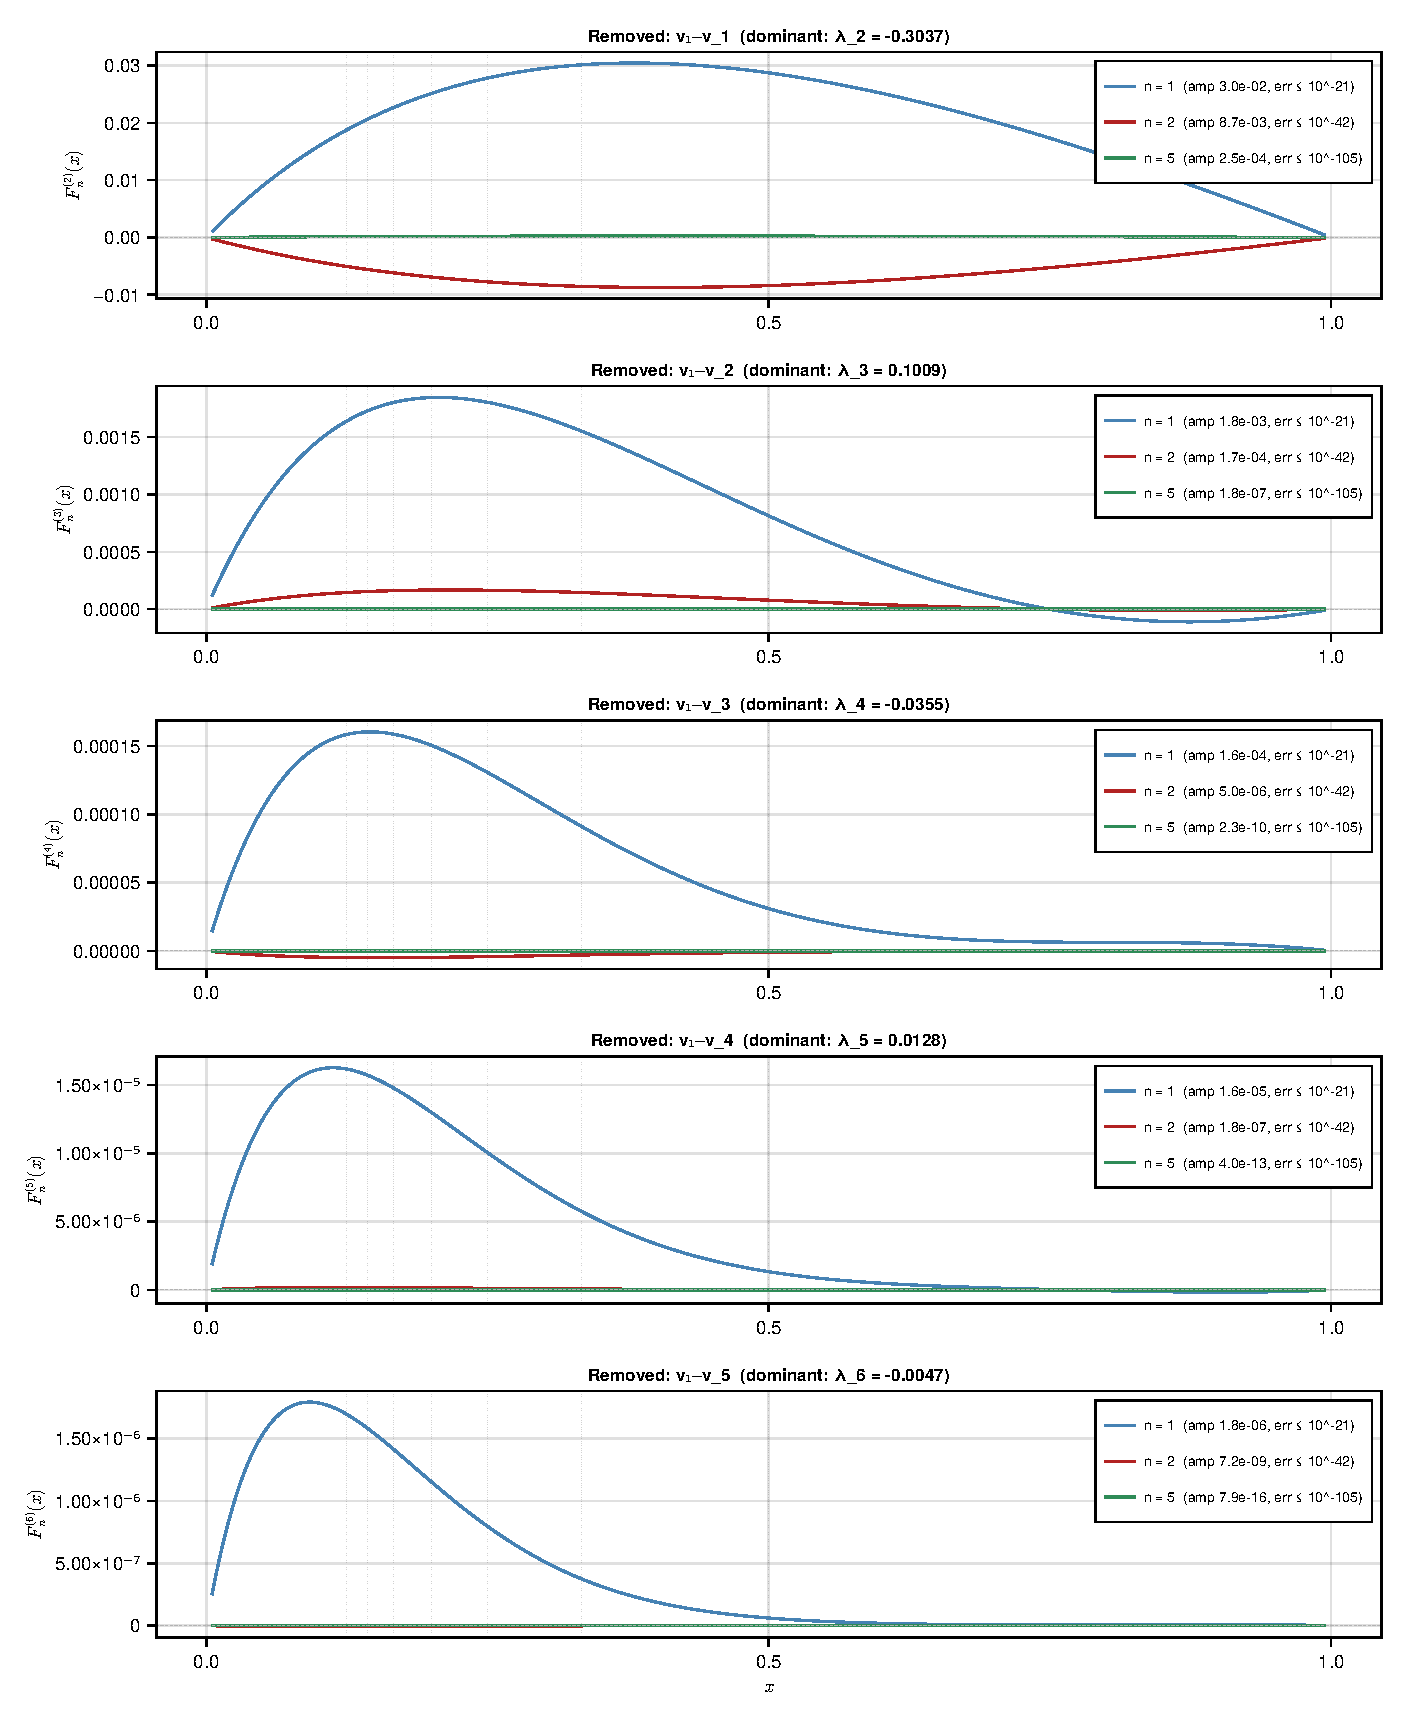
\includegraphics[width=\textwidth]{integrated_spectral_progressive.pdf}
\caption{Integrated spectral expansion $F_n^{(j_0)}(x) = \int_0^x
  \sum_{j \geq j_0} \lambda_j^n\,\ell_j(\mathbf{1})\,v_j(t)\,dt$
  with the first $j_0 - 1$ eigenfunctions cumulatively removed.
  Each panel shows $n = 1$ (blue), $n = 2$ (red), $n = 5$ (green).
  Dotted vertical lines mark the Markov partition boundaries $x = 1/k$.}
\label{S-fig:integrated-spectral}
\end{figure}

\clearpage
\subsection*{Eigenfunction Structure and the Markov Partition}

The Gauss map $G(x) = \{1/x\}$ admits a countable Markov partition into
cylinders $I_n = [1/(n+1), 1/n]$ for $n = 1, 2, 3, \ldots$.
We investigate the relationship between the eigenfunctions $v_j$ and
this partition by analysing zero crossings and local extrema.

\medskip\noindent
\textbf{Zero crossings.}
The invariant density $v_1$ is strictly positive on $(0,1)$, as expected.
For $j \geq 2$, the eigenfunction $v_j$ has a small number of zero crossings:
odd-indexed eigenfunctions typically have~$2$ zeros, even-indexed have~$1$ or~$3$.
The first zero of $v_j$ sits near $x \approx 1/j$, matching the left endpoint of
the cylinder $I_{j-1}$.  For $j \gtrsim 40$, the polynomial representation in the
shifted monomial basis $\{(x-1)^k\}$ develops spurious Runge-type oscillations
at Float64 precision, producing artificially many zero crossings (e.g., ${\sim}\,2900$ for $v_{50}$).

\begin{figure}[ht]
\centering
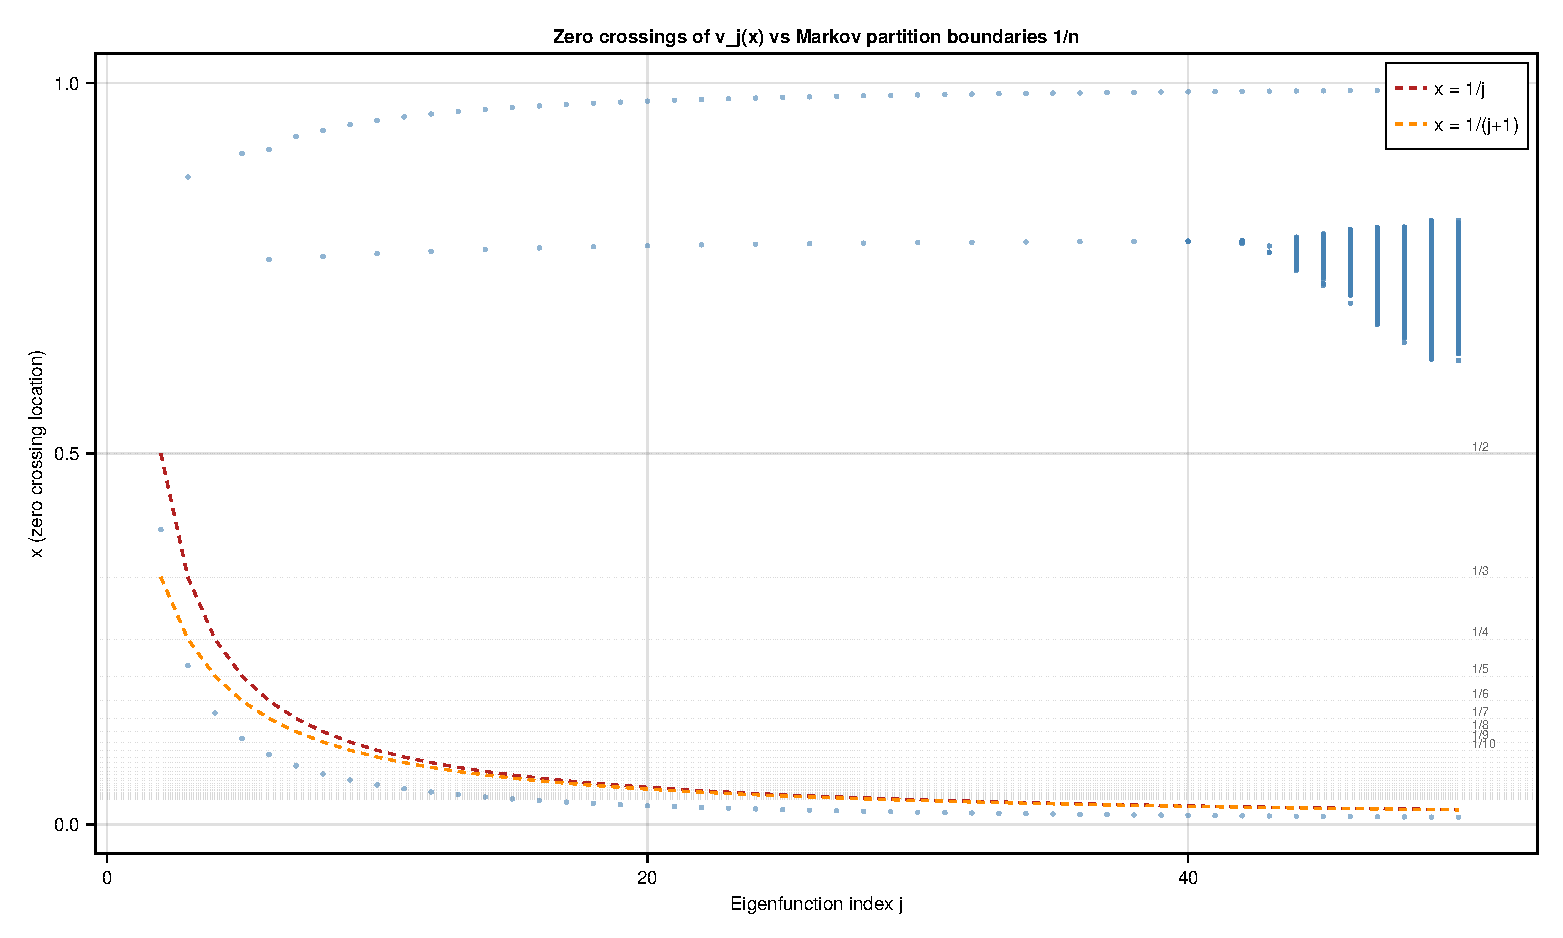
\includegraphics[width=0.85\textwidth]{eigenfunction_zero_crossings.pdf}
\caption{Zero crossing locations of $v_j(x)$ (blue dots) versus Markov
partition boundaries $x = 1/n$ (dotted grey).
The reference curves $x = 1/j$ (red dashed) and $x = 1/(j+1)$ (orange dashed) are shown.}
\label{S-fig:zero-crossings}
\end{figure}

\begin{figure}[ht]
\centering
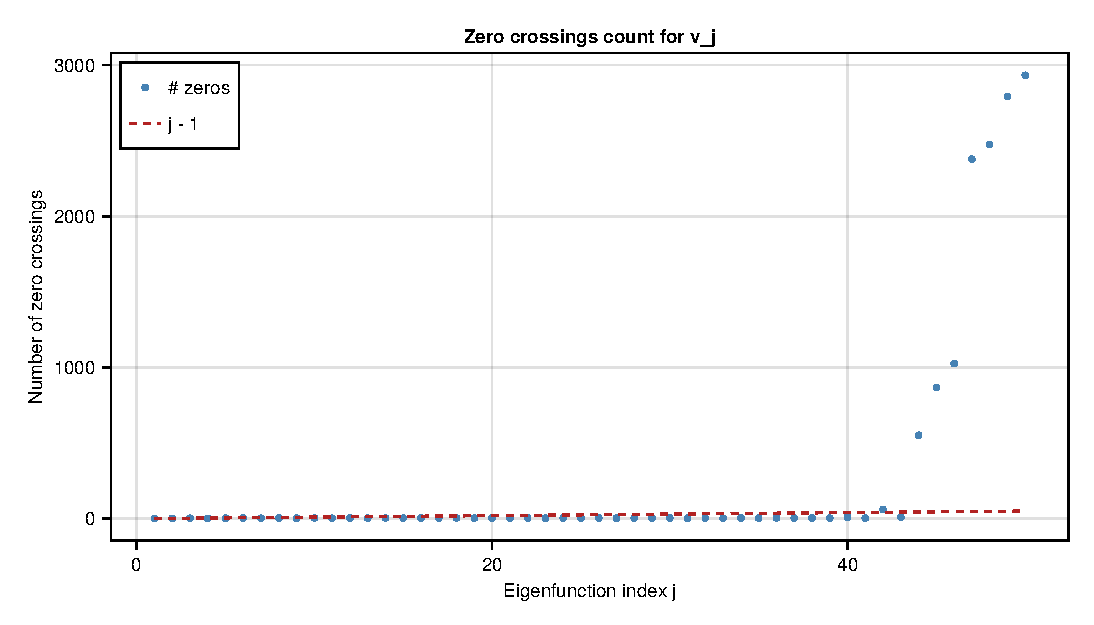
\includegraphics[width=0.7\textwidth]{eigenfunction_zero_count.pdf}
\caption{Number of zero crossings of $v_j$ versus $j$.
For $j \leq 39$ the count stays at $1$--$3$; the explosion for $j \geq 40$
is a Runge artefact of the polynomial basis at Float64 precision.}
\label{S-fig:zero-count}
\end{figure}

\medskip\noindent
\textbf{Dominant local extremum.}
For each $j \geq 3$, the largest local extremum (in absolute value)
of $v_j$ is located near the Markov boundary $x = 1/j$:
\[
x_{\max}(v_j) \;\approx\; \frac{1}{j}.
\]
For $j = 3, \ldots, 24$, the extremum lies slightly above $1/j$, inside $I_{j-1} = [1/j, 1/(j-1)]$;
for $j \geq 25$, it drifts slightly below $1/j$, into $I_j = [1/(j+1), 1/j]$.
The relative error $|x_{\max}(v_j) - 1/j|/(1/j)$ is tabulated below for selected~$j$:

\medskip
\begin{center}
\begin{tabular}{rcccc}
\toprule
$j$ & $x_{\max}(v_j)$ & $1/j$ & rel.\ error & cylinder \\
\midrule
 3  & 0.45498 & 0.33333 & 36.5\% & $I_2$ \\
 5  & 0.23258 & 0.20000 & 16.3\% & $I_4$ \\
10  & 0.10663 & 0.10000 &  6.6\% & $I_9$ \\
20  & 0.05056 & 0.05000 &  1.1\% & $I_{19}$ \\
30  & 0.03296 & 0.03333 &  1.1\% & $I_{30}$ \\
40  & 0.02439 & 0.02500 &  2.4\% & $I_{40}$ \\
50  & 0.01932 & 0.02000 &  3.4\% & $I_{51}$ \\
\bottomrule
\end{tabular}
\end{center}

\noindent
For $j \geq 10$ the mean relative error is $2.3\%$ (std.\ dev.\ $1.5\%$);
for $j \geq 20$ it is $1.8\%$ (std.\ dev.\ $1.1\%$).
Each eigenfunction is thus ``tuned'' to the Markov boundary $x = 1/j$,
confirming that higher eigenmodes encode progressively finer partition structure.

\begin{figure}[ht]
\centering
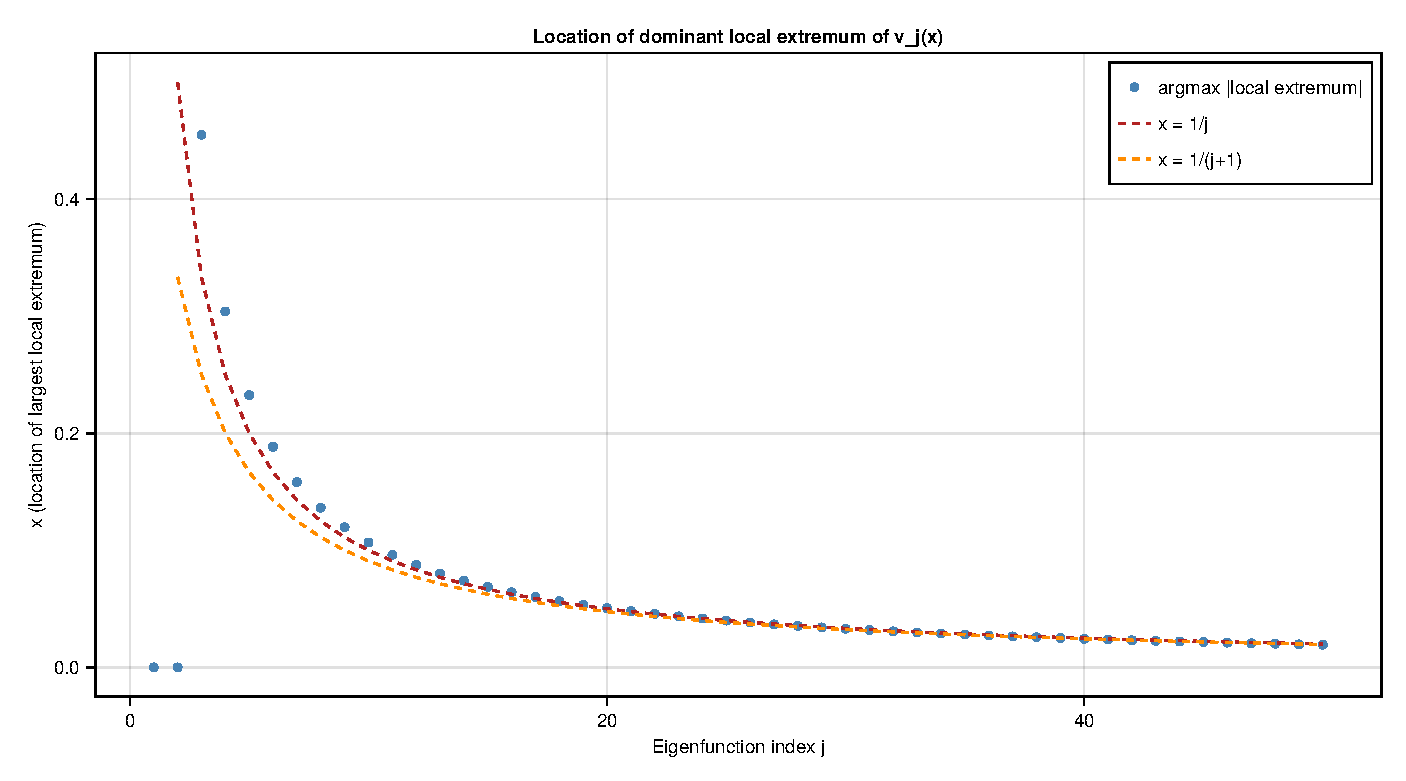
\includegraphics[width=0.85\textwidth]{eigenfunction_local_extrema.pdf}
\caption{Location of the dominant local extremum of $v_j(x)$ (blue dots)
compared with $x = 1/j$ (red dashed) and $x = 1/(j+1)$ (orange dashed).
For $j \geq 10$ the extremum tracks $1/j$ with ${\sim}\,2\%$ relative error.}
\label{S-fig:local-extrema}
\end{figure}

\clearpage
\subsection*{Non-Normality of the Transfer Operator}

The GKW transfer operator is not normal, so its Schur decomposition
$A = Q T Q^*$ has a non-trivial strictly upper triangular part.
We quantify this non-normality using the ordered Schur form with eigenvalues
sorted by decreasing $|\lambda_j|$ on the diagonal ($K = 1024$, $n = 1025$).

\medskip\noindent
\textbf{Henrici departure from normality.}
The Henrici number
\[
\delta_H \;=\; \frac{\|T - \operatorname{diag}(T)\|_F}{\|T\|_F} \;=\; 3.82 \times 10^{-1}
\]
indicates that roughly $38\%$ of the Frobenius norm of $T$ resides in the
off-diagonal entries, confirming significant non-normality.

\medskip\noindent
\textbf{Coupling structure.}
For fixed row $i$, the entry $T_{ij}$ with $j > i$ quantifies
the coupling from Schur mode $j$ (smaller $|\lambda_j|$)
back into mode $i$ (larger $|\lambda_i|$).
Figure~\ref{S-fig:schur-heatmap} shows the full $80 \times 80$ heatmap of
$\log_{10}|T_{ij}|$; Figure~\ref{S-fig:schur-rows} displays the row profiles
$|T_{i,j}|$ for selected~$i$.

\begin{figure}[ht]
\centering
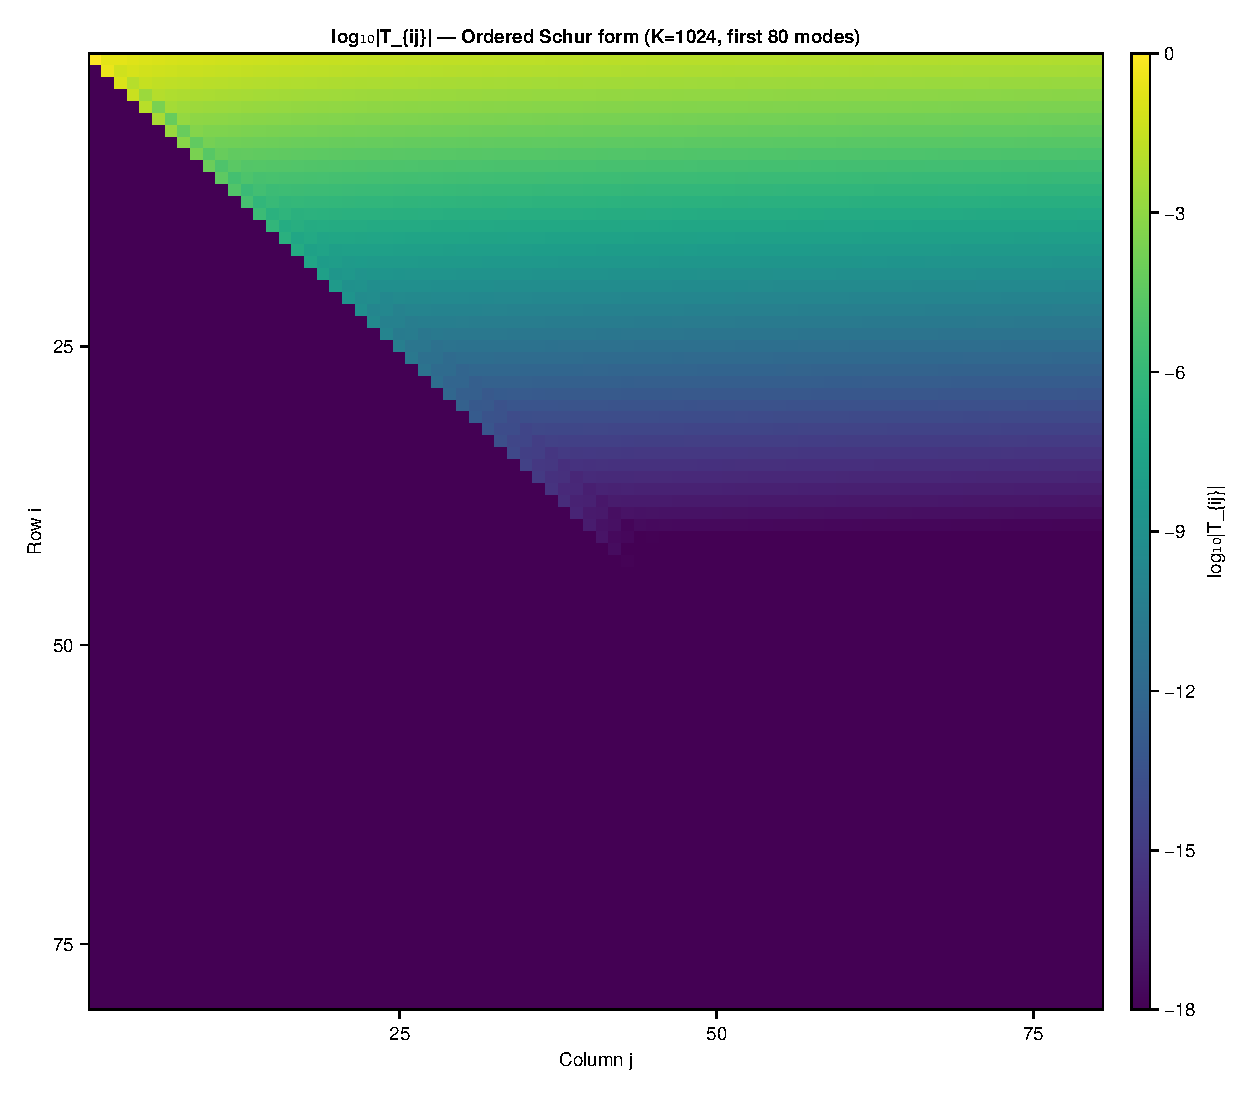
\includegraphics[width=0.75\textwidth]{schur_nonnormality_heatmap.pdf}
\caption{Heatmap of $\log_{10}|T_{ij}|$ in the ordered Schur form
(eigenvalues sorted by decreasing $|\lambda|$, first $80$ modes).
The diagonal contains the eigenvalues; the upper triangular
entries encode non-normal coupling between modes.}
\label{S-fig:schur-heatmap}
\end{figure}

\begin{figure}[ht]
\centering
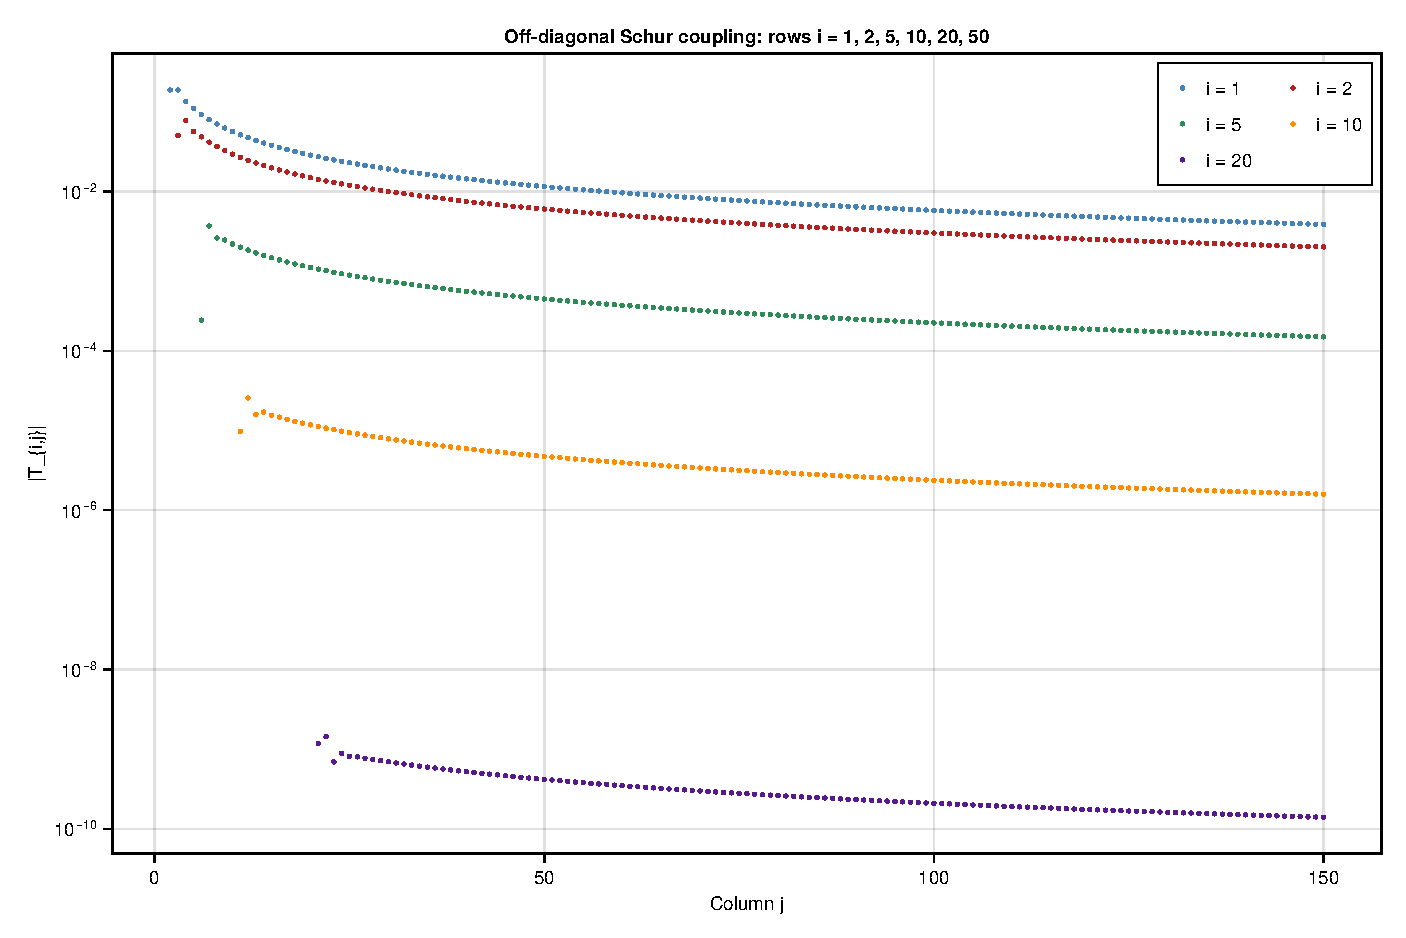
\includegraphics[width=0.85\textwidth]{schur_nonnormality_rows.pdf}
\caption{Off-diagonal Schur coupling $|T_{i,j}|$ for rows
$i = 1, 2, 5, 10, 20, 50$ (log scale).
Mode~$j$ feeds back into mode~$i$ with strength $|T_{i,j}|$.}
\label{S-fig:schur-rows}
\end{figure}

\begin{figure}[ht]
\centering
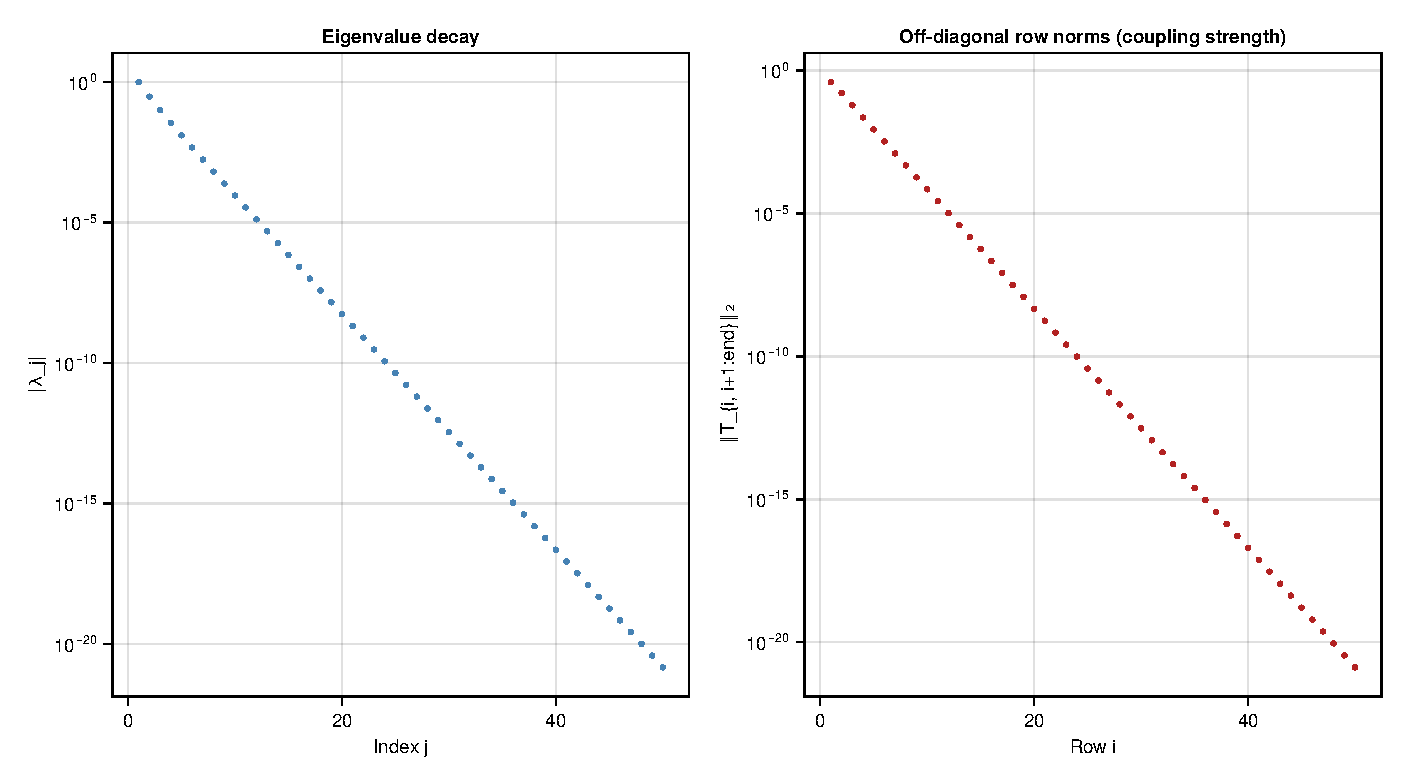
\includegraphics[width=\textwidth]{schur_nonnormality_summary.pdf}
\caption{Left: eigenvalue decay $|\lambda_j|$ versus index~$j$.
Right: off-diagonal row norms $\|T_{i, i+1:n}\|$ measuring the total
coupling strength from all higher modes into mode~$i$.}
\label{S-fig:schur-summary}
\end{figure}

\end{document}
